\documentclass[titlepage,a4pape]{jsarticle}
\bibliographystyle{junsrt}
\usepackage[dvipdfmx]{graphicx}
\usepackage{lscape}
\usepackage{here}
\usepackage{bmpsize}
\setlength{\topmargin}{10mm}
\setlength{\headsep}{0mm}
\setlength{\oddsidemargin}{-5mm}
\setlength{\evensidemargin}{-5mm}
\setlength{\textwidth}{17cm}
\setlength{\textheight}{22cm}
\setlength{\columnsep}{10mm}
\setcounter{topnumber}{5}
\def\topfraction{.7}
\usepackage{amsmath}
\usepackage{url}
\usepackage{here}
\usepackage{bm}
\makeatletter
\usepackage{comment}
\newcommand{\figcaption}[1]{\def\@captype{figure}\caption{#1}}
\newcommand{\tblcaption}[1]{\def\@captype{table}\caption{#1}}
\makeatother
\usepackage{amssymb}
\usepackage[subrefformat=parens]{subcaption}
\usepackage{longtable}
\usepackage{siunitx}
\usepackage[dvipdfmx]{colortbl}

\title{\vspace{-15mm}{\LARGE 2023年度 卒業論文}\\\vspace{25mm}
\huge
深層学習を用いた優美さ特徴の抽出
\vspace{20mm}\\}

\author{
\Large 大阪工業大学ロボティクス&デザイン工学部\\\\
\vspace{5mm}\Large ロボット工学科\\
\vspace{5mm}
\vspace{0mm}\\
{\huge 薮田 千尋} \vspace{14.5mm}\\
\\\Large 指導教員\\\\\vspace{-4.0mm}
\vspace{0mm}\Large 上田悦子
}
\date{}


\begin{document}
\maketitle
\newpage

\setlength{\baselineskip}{16pt}
\fontsize{12pt}{20pt}\selectfont
\pagenumbering{roman}
\setcounter{page}{1}
\tableofcontents

\newpage

\listoffigures

\newpage

\listoftables
\newpage

\pagenumbering{arabic}
\newpage
\bigskip
\newpage

\section{はじめに}
\section{はじめに}

\subsection{研究背景}
近年,深層学習は大きな発展を見せている.
Recurrent Neural Network\cite{rnn}はConvolutional Neural Network\cite{cnn}にはない
「時間」という概念を持ち,機械翻訳の分野で大きな成果を出した.
一方で,小説などの大きな入力には対応できないという欠点もあった.
RNNに長期的記憶の概念を導入したLSTM\cite{lstm}やGRU\cite{gru}も開発されたが,
計算時間の増加が問題であった.

2017年に登場したTransformer\cite{transformer}は単純な行列計算のみで完結したネットワークで,
機械翻訳でこれまでのRNNを超える精度を出し,計算時間も大幅に削減したことで,
機械翻訳のデファクトスタンダードとなった.
2020年にはVision Transformer\cite{vit}が開発され,画像認識でCNNを超える精度を出した.
さらに翌年にはVideo Vision Transformer\cite{vivit}が開発され,動画解析でもRNNを超える精度を出した.

AIの活躍は単純なタスクに留まらない.ボードゲームでは,
囲碁のAlphaGo\cite{alphago},その後継でフレームワークとして
開発されたAlphaZero\cite{alphazero}は囲碁,チェス,将棋で成果を上げた.
芸術ではMusic Transformer\cite{mut}で作曲,DALL-E2\cite{dalle2}で
図\ref{astronaut}のような作画が可能となった.

\begin{figure}[b]
  \begin{center}
    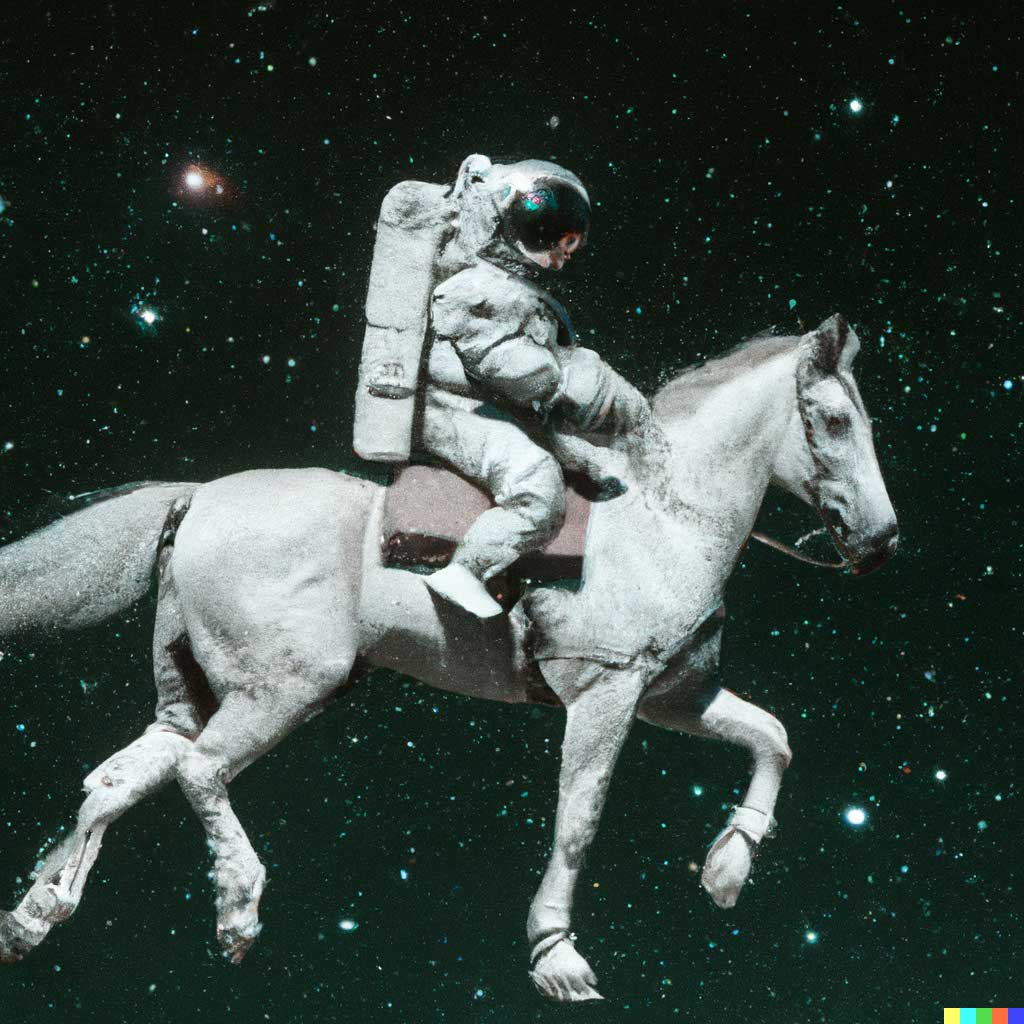
\includegraphics[width=60mm]{images/quote/astronaut.jpg}
  \end{center}
  \caption[単語から生成されたDALL-E2の作画]{単語から生成されたDALL-E2の作画\cite{demo}}
  \label{astronaut}
\end{figure}
\clearpage

\begin{figure}[t]
  \begin{center}
    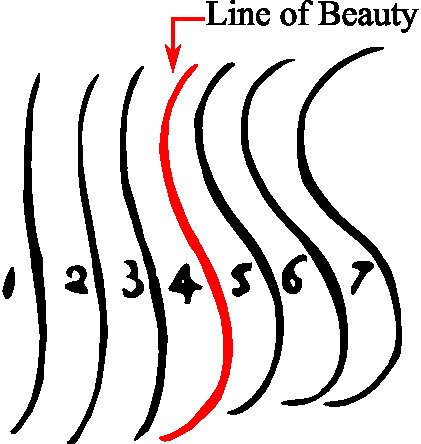
\includegraphics[width=60mm]{images/quote/hogarth_curve.pdf}
  \end{center}
  \caption{Hogarth Curve}
  \label{hogarth_curve}
\end{figure}

単純作業,ボードゲーム,果ては芸術まで人間を凌駕するまでに成長したAI,人間の判断は
必ずしも正しいとは言えなくなってきている.
所属するヒューマンモデリング研究室では
長年「優美さ」の定量化を目標に様々なアプローチが試されてきた.
「優美さ」とは,人間の動作を表現する形容詞である.
Buytendijk\cite{buytendijk}は,優美な動作とは
\begin{enumerate}
  \item ゆっくりとした,丸みのある動き
  \item 持続性と流動性を持つ動き
  \item 緊張と解繁がリズミカルに交替して現れる動き
\end{enumerate}
であると主張した.
また,Hogarth\cite{hogarth}は,図\ref{hogarth_curve}のような「美の線」を多く含むものであると主張した.

しかし,同研究室では未だ深層学習を用いたアプローチはなされていない.
また,上記定義やこれまでのアプローチは人間の主観評価をベースにしている.
ここで,AIを用いて優美さを特定しようとした場合どのような結果をもたらすのか,疑問に思った.
「優美さ」の根底にある判断根拠とは一体どんなものなのか,
従来の結果とどのような相違点または共通点が存在するのかを特定するために今回の研究を行った.
\clearpage

\subsection{研究目的}
我々の研究室ではHogarthの規範に則り,動作解析や動作生成を行ってきた.
稲津\cite{inazu}は手先の軌道をB-spline近似\cite{bspline}したのちに
\begin{enumerate}
  \item 軌道長がより長い
  \item Hogarth Curveとの形状類似度
  \item 両弧の弧長がほぼ等しい
  \item 両弧の全曲率が0.873〜1.44
\end{enumerate}
を検証する評価モデルを提案した.

照岡\cite{teruoka}は強化学習を用いて曲線の生成を試みた.図\ref{robot_arm}のような
シミュレータ上で駆動する仮想ロボットアームを,強化学習から生成される動作で動かした.
目標点との位置差分と各関節の加速度を用いて,照岡の提案する様々な報酬関数で学習を進めた.
それらの動作を同じくB-spline近似し,稲津の評価モデルで優美さを検証した.

\begin{figure}[b]
  \begin{center}
    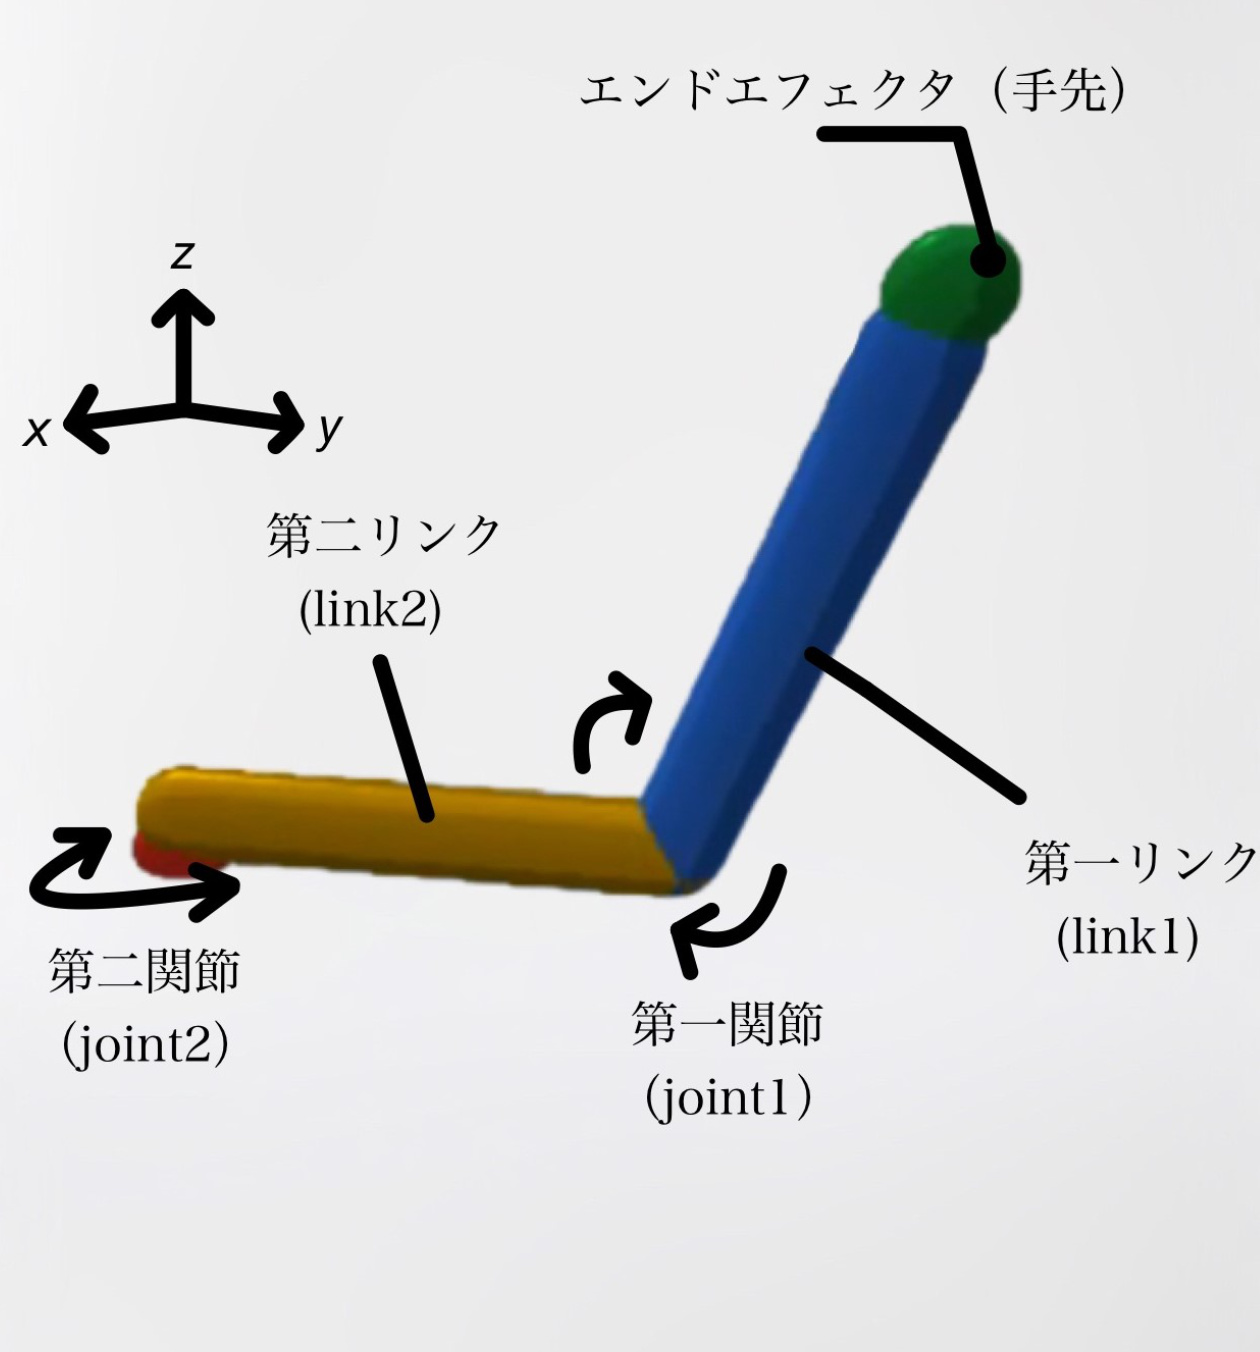
\includegraphics[width=70mm]{images/quote/robot_arm.png}
  \end{center}
  \caption{実装した2自由度ロボットアーム}
  \label{robot_arm}
\end{figure}
\clearpage

これらの研究は手先軌道に限定して着目したもので,論文内でも他部位との関係検証の必要性や
特定状況下でしか機能しないことが言及されている.
実際,上田研では実データとして既存のcsvデータを使用するにとどまっていた.
さらに最終的な優美評価はアンケートによる主観評価で,これもデータ量として少ないものであった.

深層学習を用いることでデータに依存しないネットワーク構築が可能であり,
データが増えるほど精度が上がることが期待できる.
さらに,mp4を実データとすることでデータ収集も容易かつ大量に行うことが可能となった.
動画全体を対象とすることでこれまで検証できなかった網羅的検証も可能となり,
従来の解析手法との比較から得られる相違点,共通点が明瞭となる.

そこで深層学習の実用性を検証するために,深層学習の精度向上及び判断根拠の可視化を本研究の目的とする.

\subsection{研究構成}
第2章では開発した舞踊分類ネットワークの構造及び学習に使用した動画データを記載した.
このネットワークは動画を[優美なダンス,普通のダンス,その他の動作]に分類することを目的とするが,
通常のAIのように精度を100\%に近づけることを目指さない.
Buytendijkの定義やHogarthの定義は動作の始点から終点を観測した時に生じるものであるから,
動作が完結したと思われるまで優美であるかどうかは判断できない.
また,ダンスにはしばしば静止した状態を保つ表現技法が用いられる.
これも優美さとは動作から生まれるものと定義されているため,判断できない.
これらのため,ダンス全体,動画の内容全てを優美と決定づけることは不可能である.
その上で,動画を3つのカテゴリに分類し,それぞれのエッセンスを取り出すことを試みた.

第3章では第2章で得たエッセンスを元に動画のどこから優美であるかを判断したのか検証した.
用いた手法として,Grad Cam\cite{gradcam}と確率分布を提案した.
Grad CamとはCNNの可視化手法であるCam\cite{cam}に勾配情報を追加して検証する手法である.
勾配を使用するため,画像でははっきりと見えていた判断根拠が,入力の大きな動画では
離散することが考えられる.
動画という時間に依存したデータであることと,出力がsoftmaxによる確率であることから,
動画全体の確率分布をグラフに起こし,どの辺りが確率が高まっているかを確認することで
判断根拠を特定しようとする試みも合わせて行った.

第4章では本研究の総括と今後の展望についてまとめた.

\clearpage
\section{舞踊分類ネットワーク}
\subsection{モデル概要}
入力された動画を[優美なダンス,普通のダンス,その他の動作]に分類するネットワークを作成した.
ネットワーク内での分類手順として
\begin{enumerate}
  \item 動画を下記で説明する二値化手法で編集する.
  \item 二値データと,それに対応するピクセル番号を畳み込む.
  \item 二つのデータを足し合わせる.
  \item Transformer Encoderに通した後,全結合し,Softmaxにかける.
\end{enumerate}
のような順序で計算した.
最適化アルゴリズムにAdam\cite{adam},損失関数に交差エントロピー誤差(\ref{entropy})を使用した.
\begin{equation}
  H(p, q) = -\sum_{i}p_i\log q_i
  \label{entropy}
\end{equation}
プログラミング言語にPython,モジュールは主にPytorch,Numpy,Cv2,Pickleを用いた.

\begin{figure}[b]
  \begin{center}
    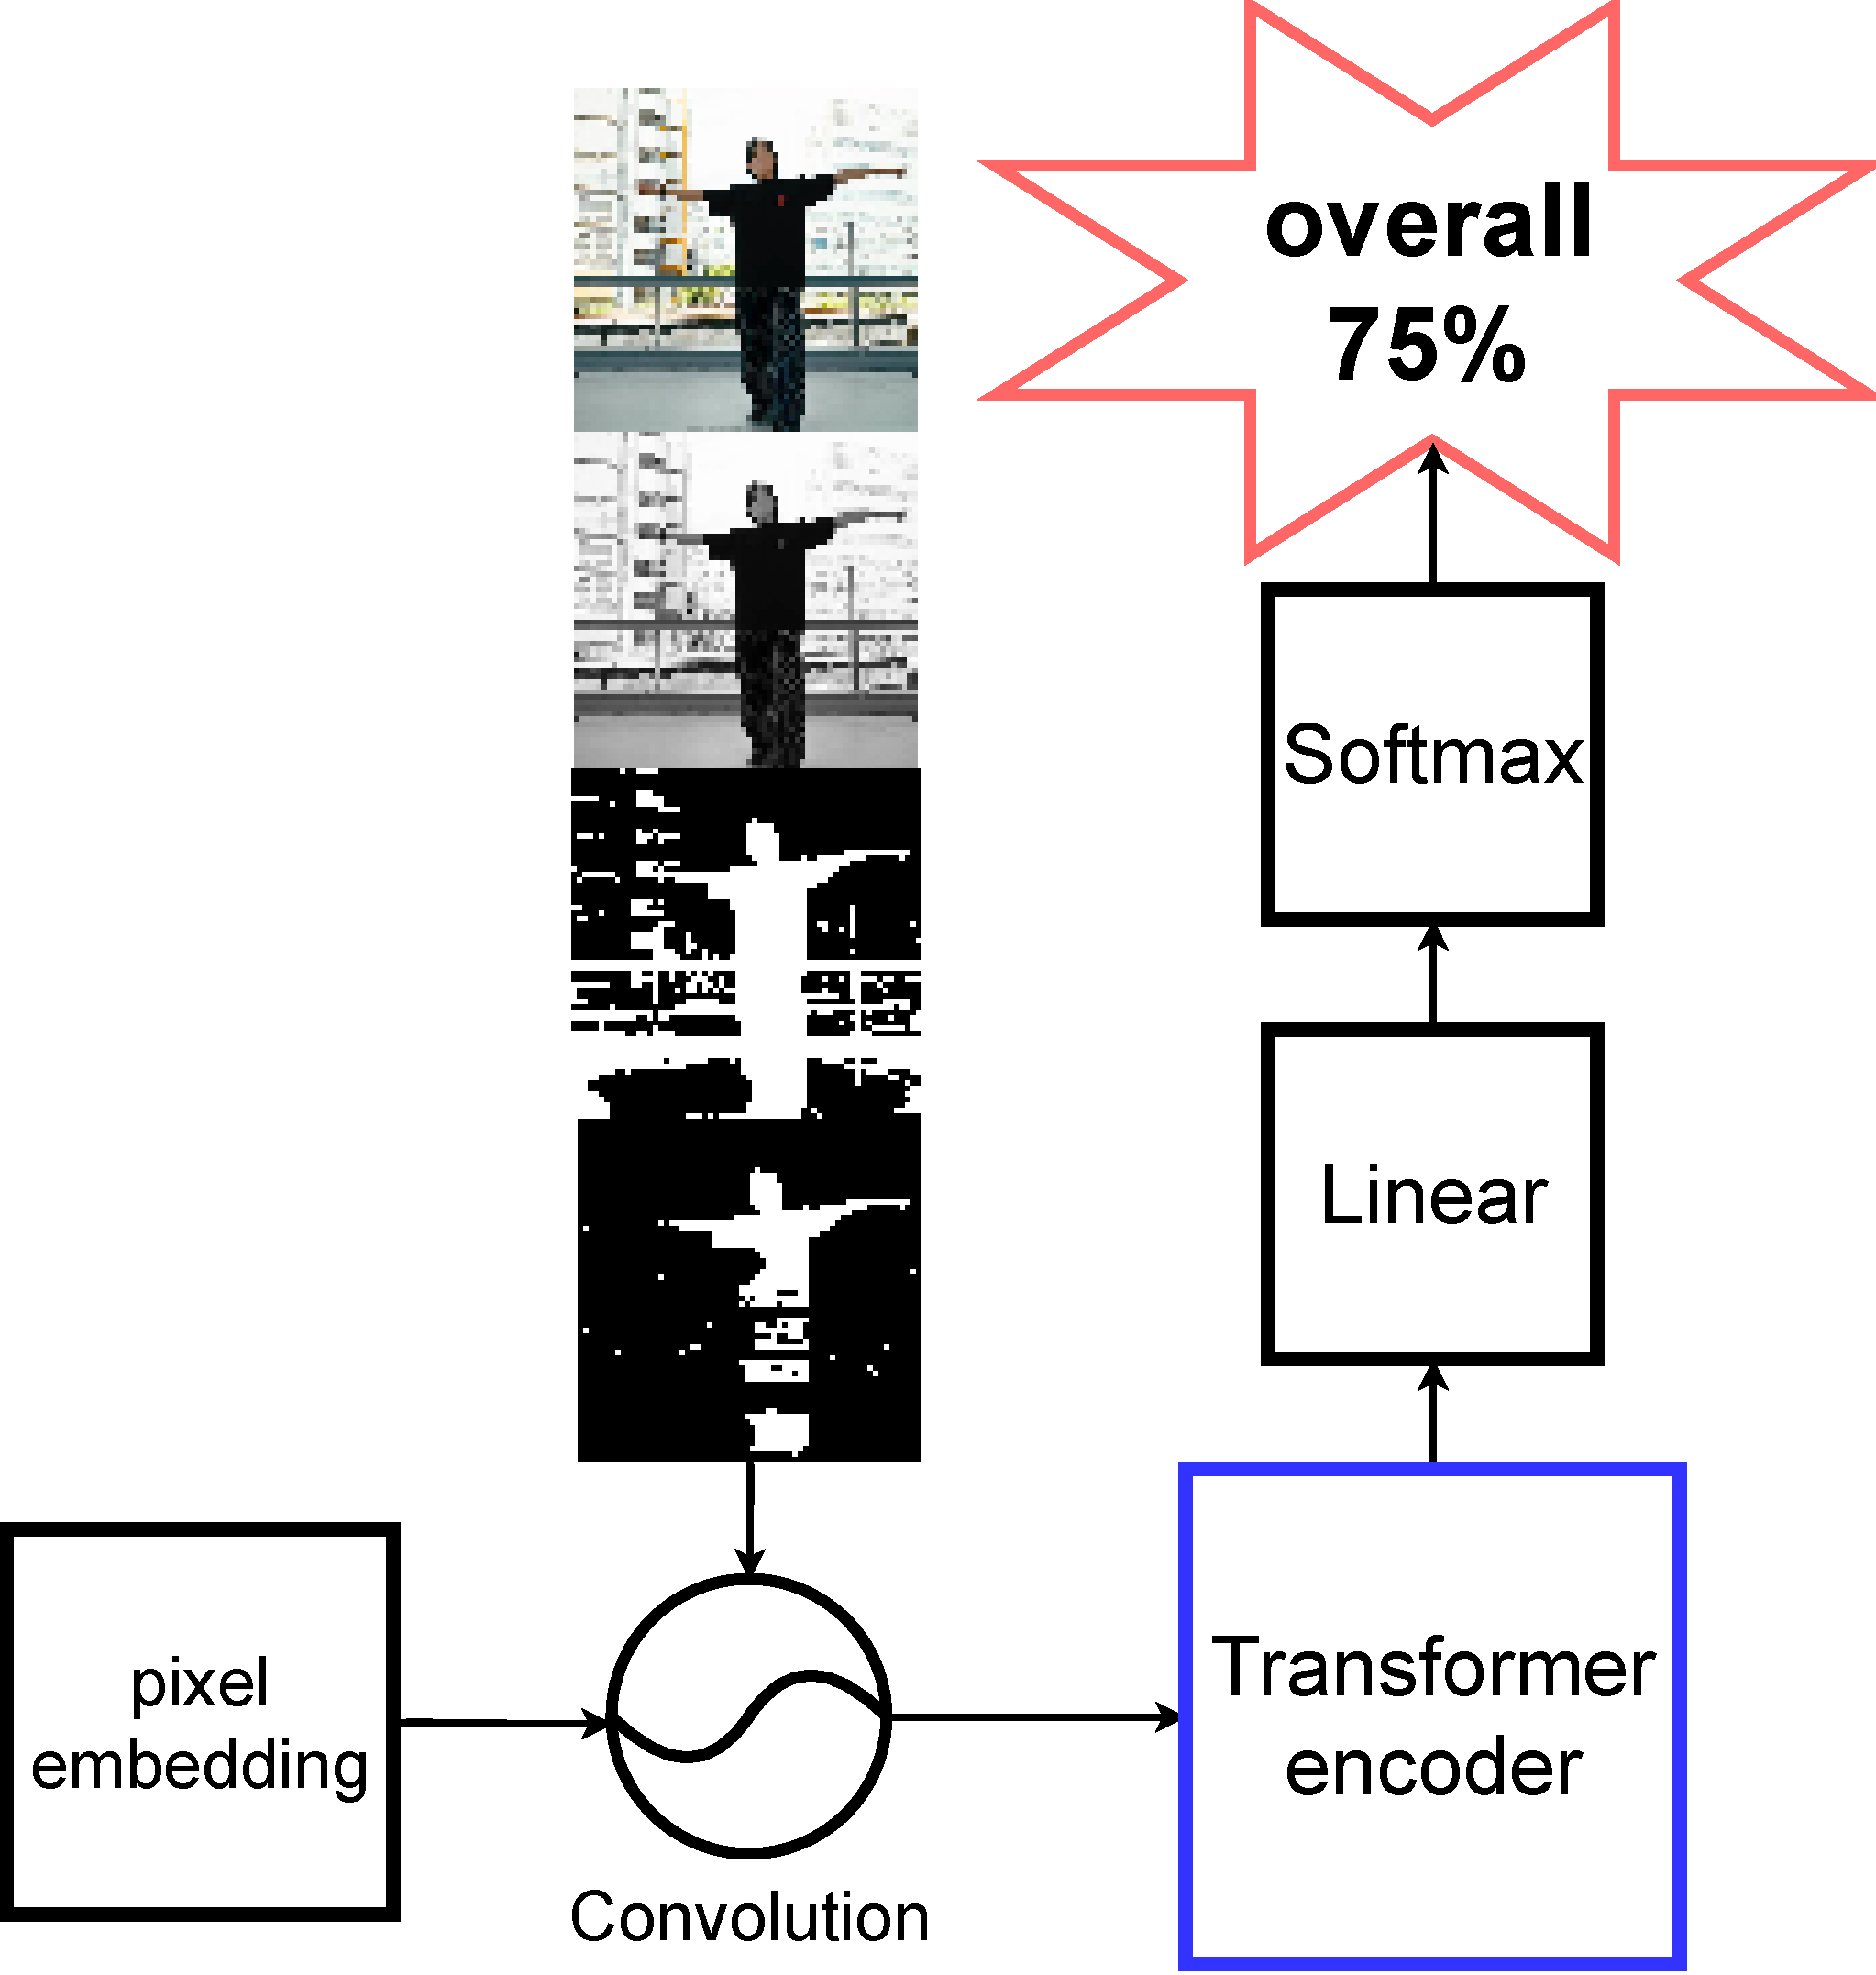
\includegraphics[width=80mm]{images/easy_chart.pdf}
  \end{center}
  \caption{モデル概要}
  \label{easy_chart}
\end{figure}

\clearpage

\subsection{使用する動画データ}
動画は\ref{video_data}を使用した.
\begin{table}[t]
  \begin{center}
    \begin{tabular}{|c|c|c|} \hline
      \ & 学習用 & 推論用 \\ \hline
      優美なダンス
        & \cite{jpn}\cite{china}\cite{ballet}\cite{thai}\cite{jpn2}
        & \cite{balletgroup}\cite{jpngroup}\cite{chinagroup}\cite{belly}
      \\ \hline
      普通のダンス
        & \cite{ariana}\cite{kadokawa}\cite{bts}\cite{manolo}\cite{aito}
        & \cite{btsgroup}\cite{arashi}\cite{hyoga}\cite{legit}
      \\ \hline
      その他の動作
        & \cite{radio}\cite{posing}\cite{boxing}\cite{running}\cite{shinkokyu}\cite{leaves}
        & \cite{radio2}
      \\ \hline
    \end{tabular}
  \end{center}
  \caption{使用した動画データ}
  \label{video_data}
\end{table}

\subsection{ネットワーク構造}

\subsection{精度}

\clearpage
\section{優美動作の評価}
\section{優美動作の評価}

\subsection{従来手法}
ヒューマンモデリング研究室ではこれまで多くのモデルが提唱されてきた.
その多くは稲津\cite{inazu2}の全曲率計算を起源としている.
先に挙げたB-spline近似で手先軌道を曲線近似し,図\ref{curves}のように
全曲率$\mu$が0.87〜1.31となる曲線を多く含むものを優美としている.
そこから面積や角度に派生するモデルも存在するが,根底は手先軌道である.
今回作成したネットワークが「優美」と判定したものは動画のどの箇所を根拠に
「優美」と判断したのか,動作を抽出して検証する際,どこに着目すべきと
示唆しているかなどを検証し,その相違点,共通点を特定した.

\begin{figure}[b]
  \begin{center}
    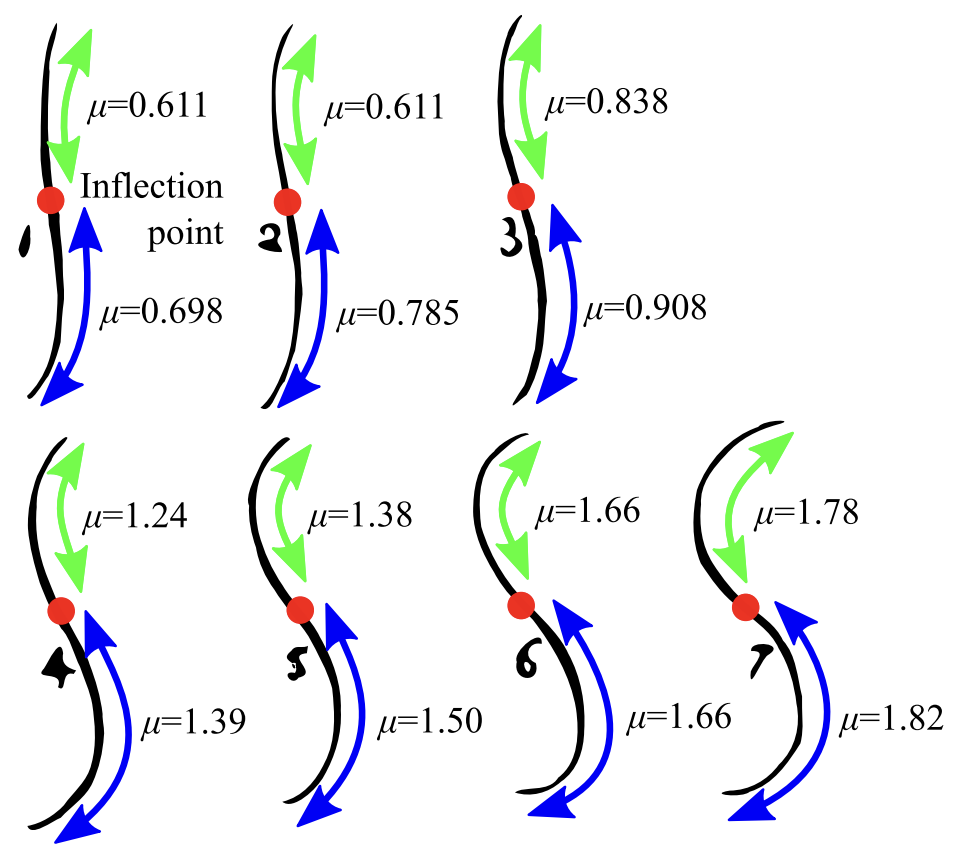
\includegraphics[width=100mm]{images/quote/curves.png}
  \end{center}
  \caption{Hogarth Curveの全曲率}
  \label{curves}
\end{figure}

\subsection{Grad Camを用いた評価}
作成したネットワークの判断根拠を可視化するために,Pytorch-GradCam\cite{pygradcam}を
使用した.作成したネットワークはPytorch\cite{pytorch}でできているので,GradCamも
同じくPytorchでできたものを使用した.

Pytorch-GradCamは入力データに対して,どのように各層が影響するかを順伝播で確認してから,
逆伝播で影響の強弱を1以下の数値で返す.今回のネットワークでは動画をフレームごとに区切るので,
1フレームずつ処理すると図\ref{camgraph}のように最大30回重複するデータが存在する.
よって出力された結果を順番に足し合わせ,特定のデータについて足し合わされた回数で各値を割り,
データの均一化を図った.データは1以下の値を取るので,255倍してデータの強弱を動画として可視化した.
また,数値は小さいが,データが離散しているので閾値0.4以下の値は0とした.

\begin{figure}[b]
  \begin{center}
    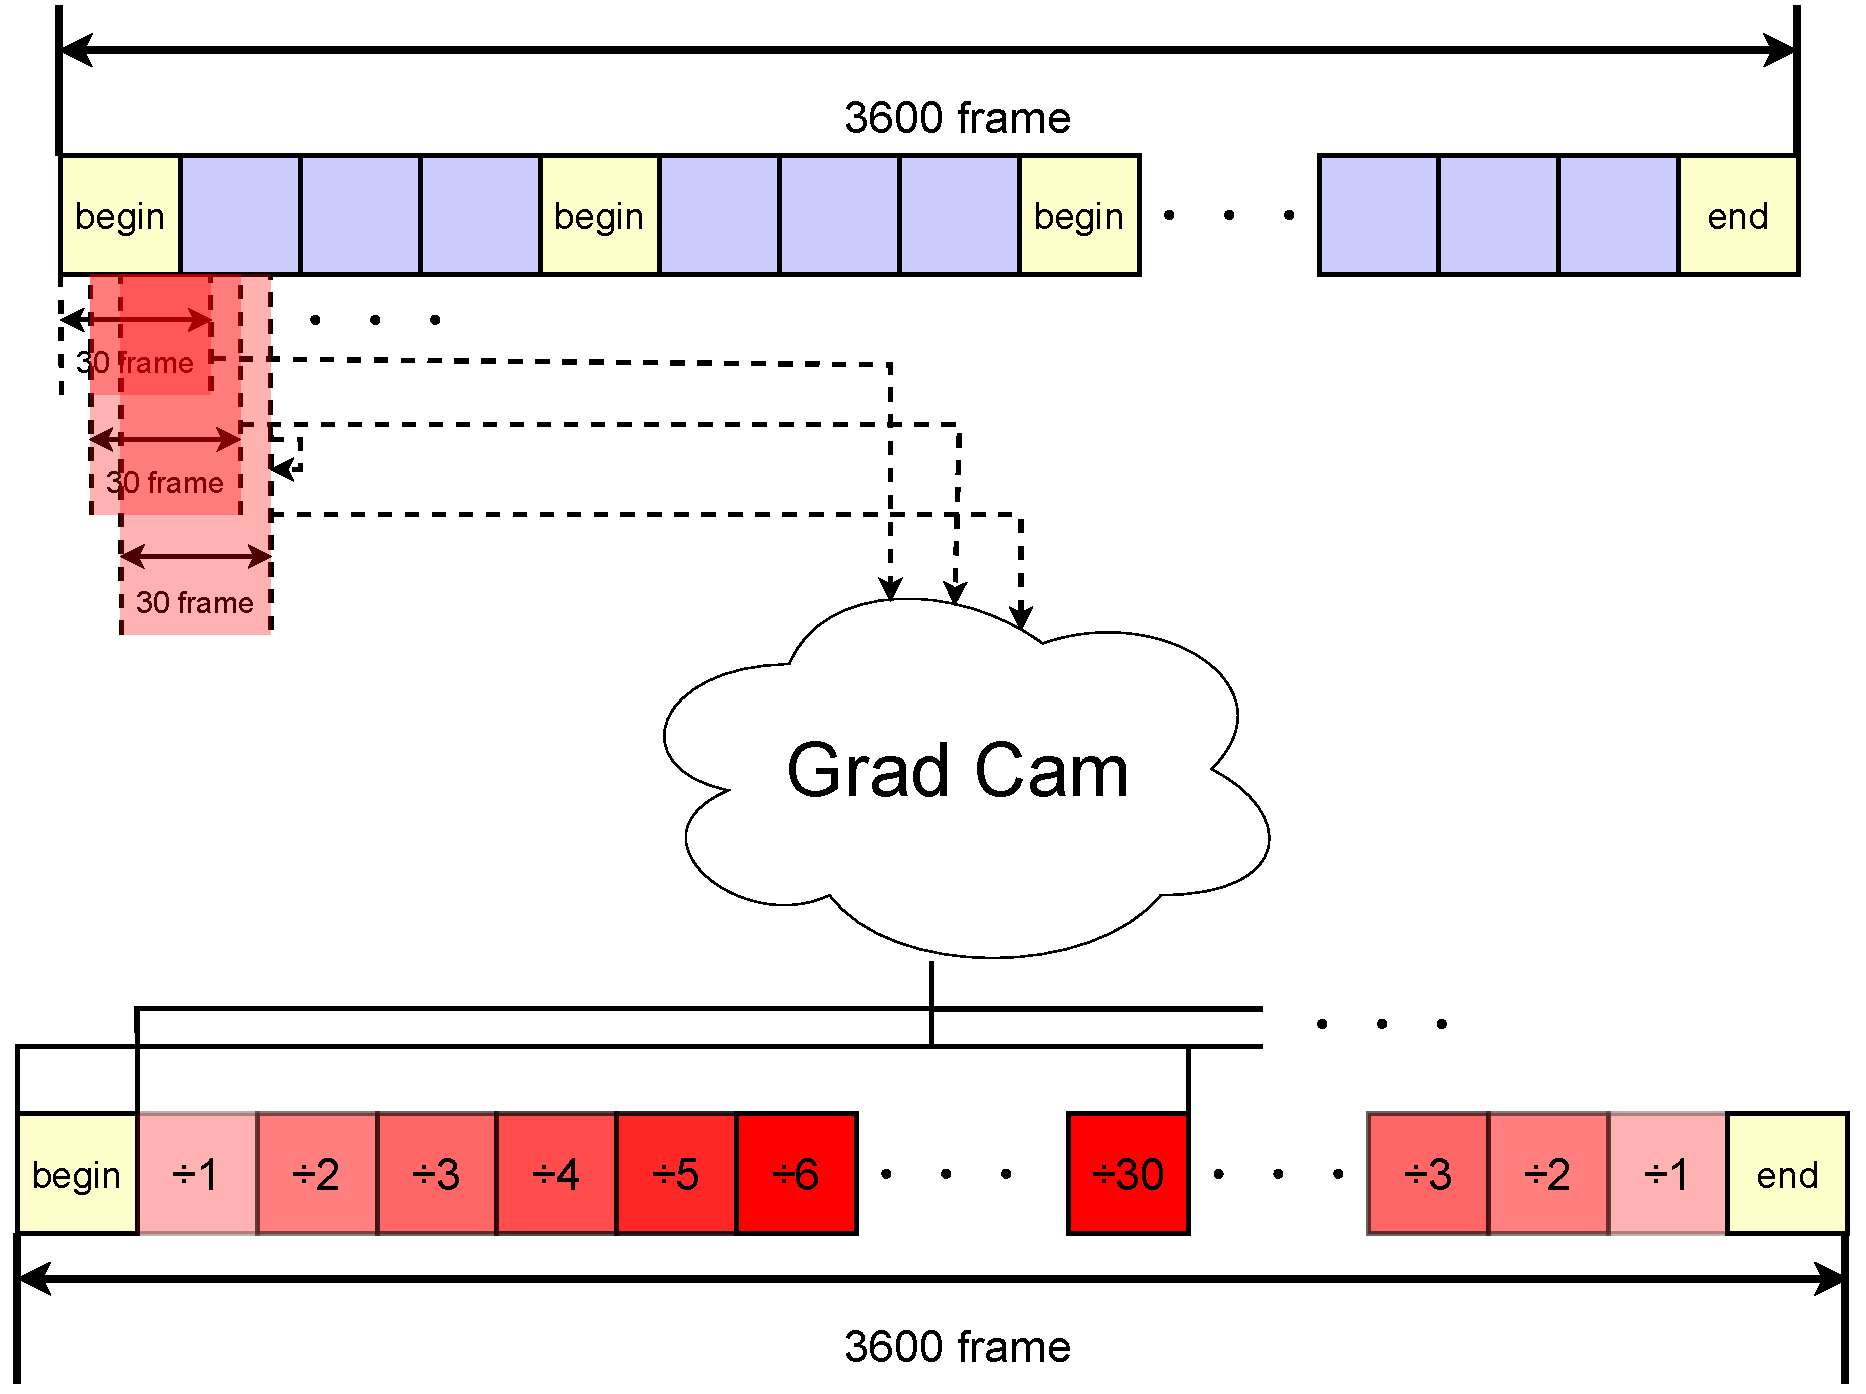
\includegraphics[width=120mm]{images/chart/gradcam.pdf}
  \end{center}
  \caption{Grad Camから出力される結果の整形方法}
  \label{camgraph}
\end{figure}
\clearpage

\begin{table}[t]
  \begin{center}
    \begin{tabular}{|c|c|c|} \hline
      \begin{minipage}[b]{3cm}
        \centering
        優美なダンス
        \vspace*{1cm}
      \end{minipage}
        & 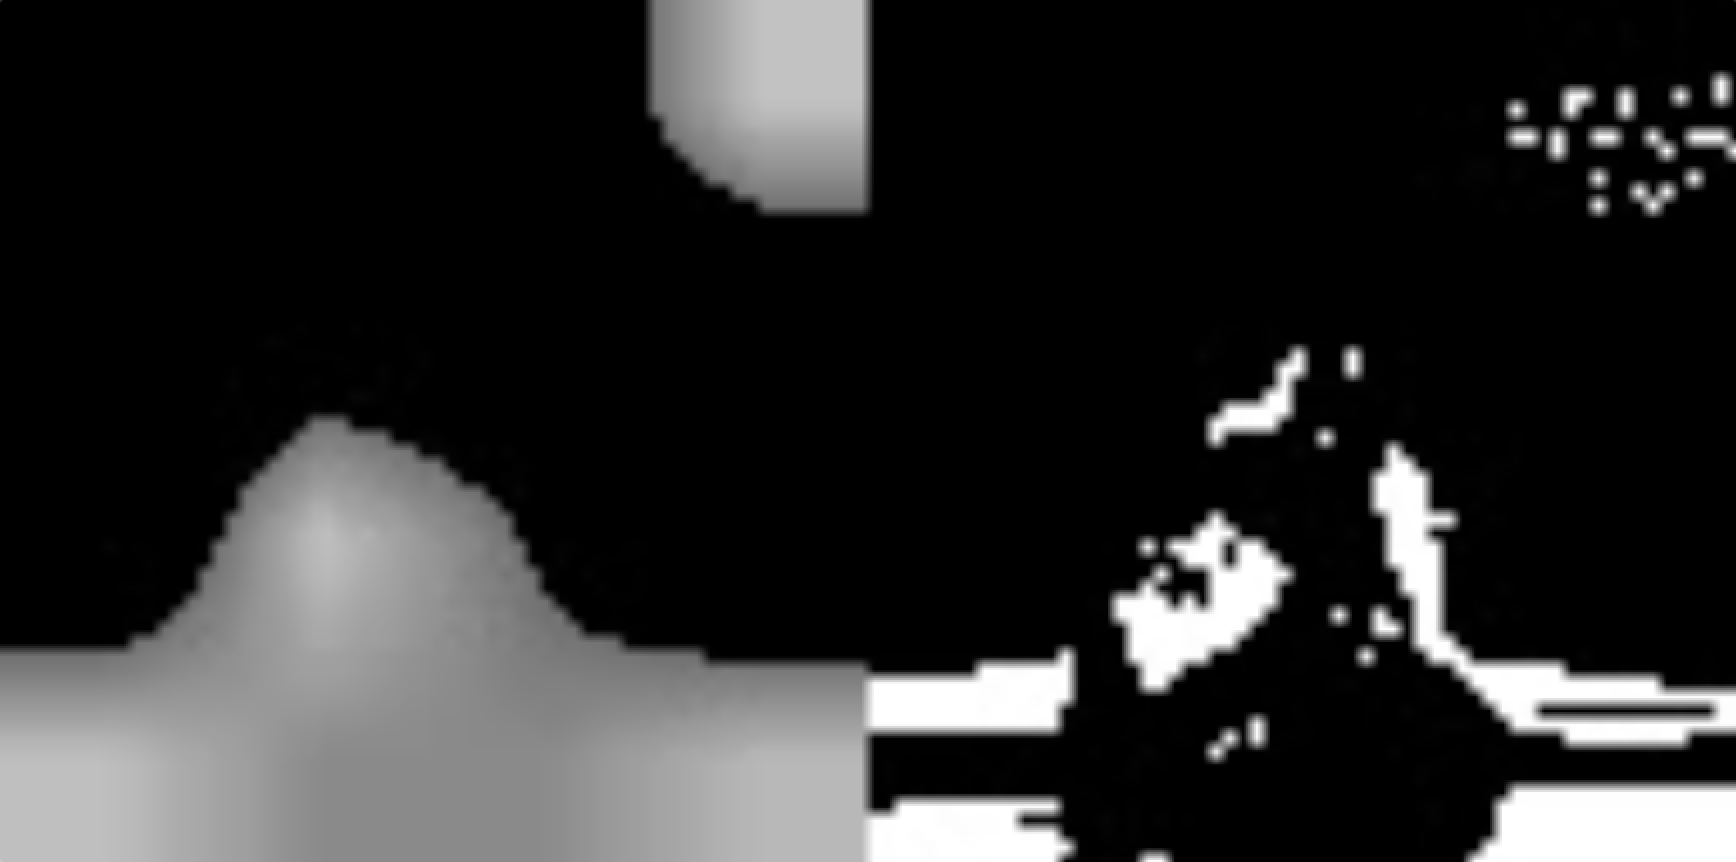
\includegraphics[width=50mm]{images/cam/chinese.png}
        & 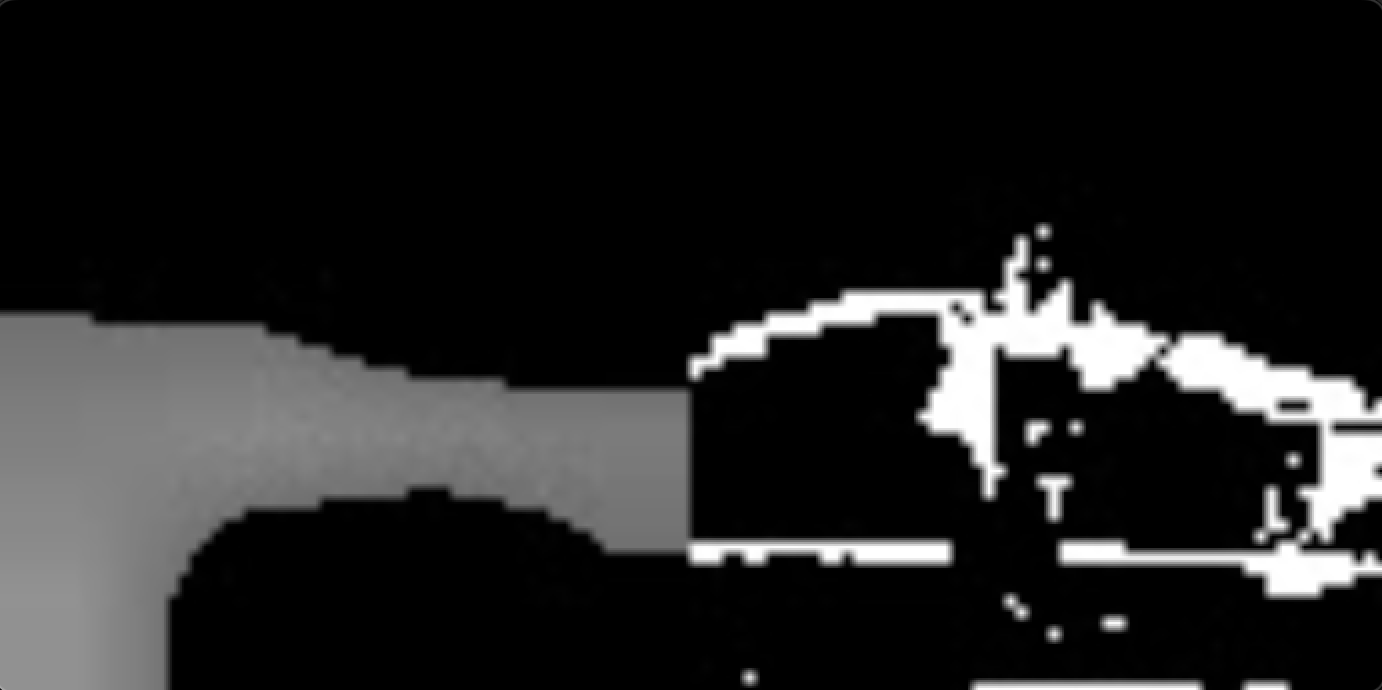
\includegraphics[width=50mm]{images/cam/japanese.png}
      \\ \hline
      \begin{minipage}[b]{3cm}
        \centering
        普通のダンス
        \vspace*{1cm}
      \end{minipage}
        & 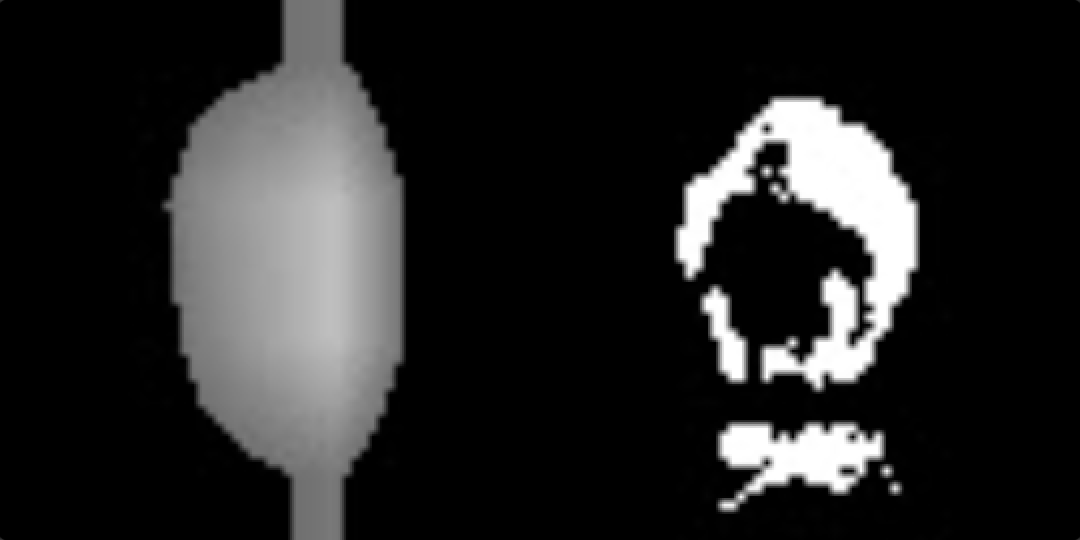
\includegraphics[width=50mm]{images/cam/kadokawa.png}
        & 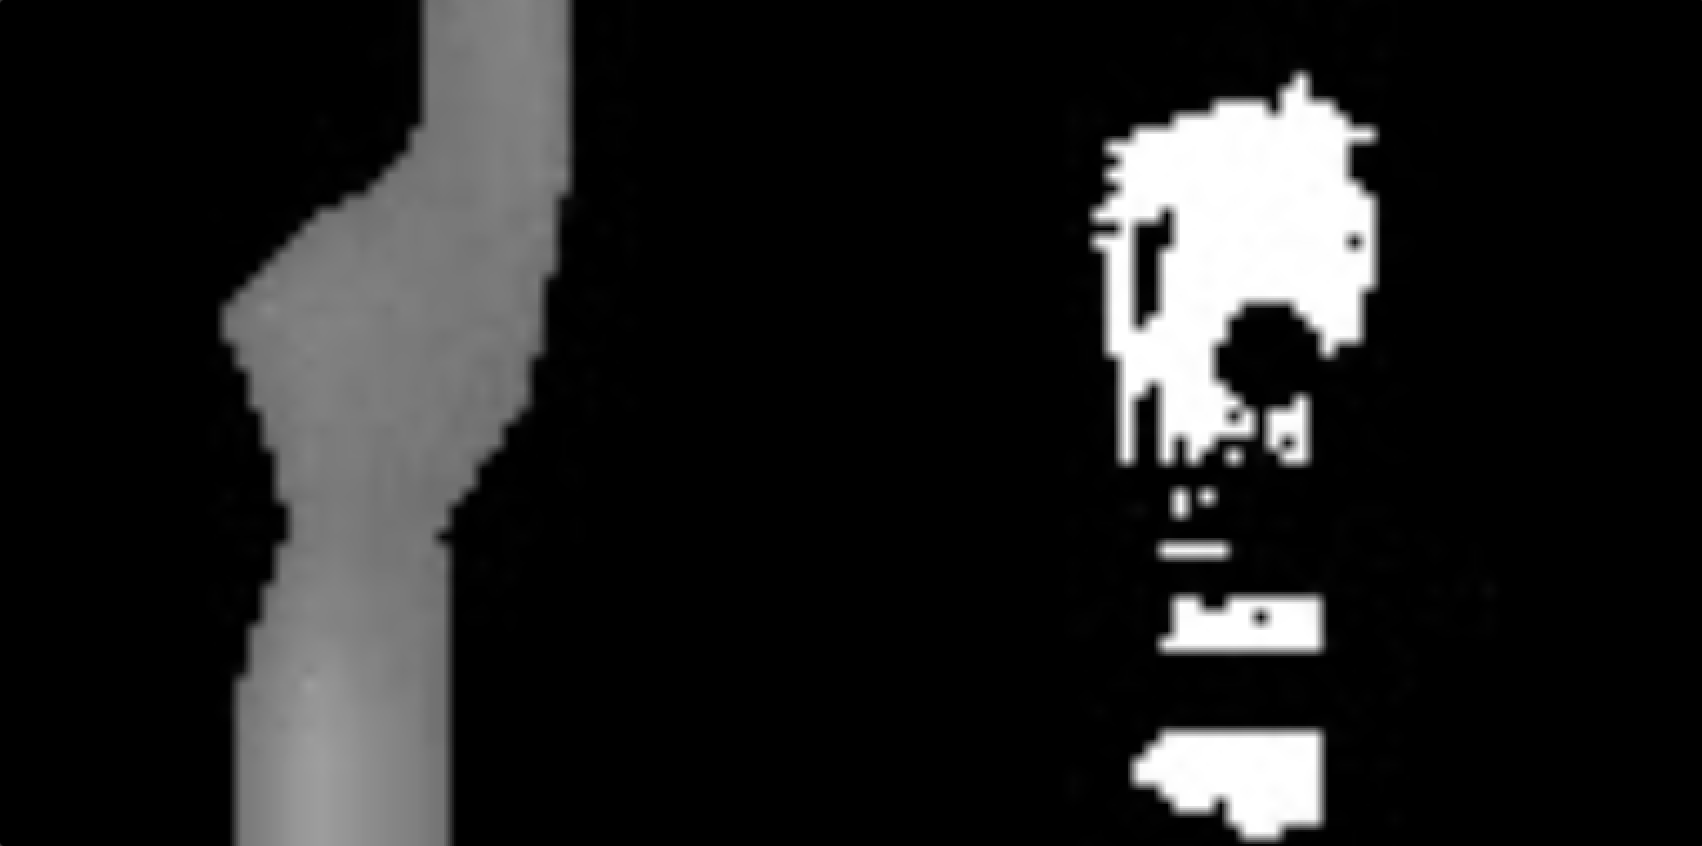
\includegraphics[width=50mm]{images/cam/aito.png}
      \\ \hline
      \begin{minipage}[b]{3cm}
        \centering
        その他の動作
        \vspace*{1cm}
      \end{minipage}
        & 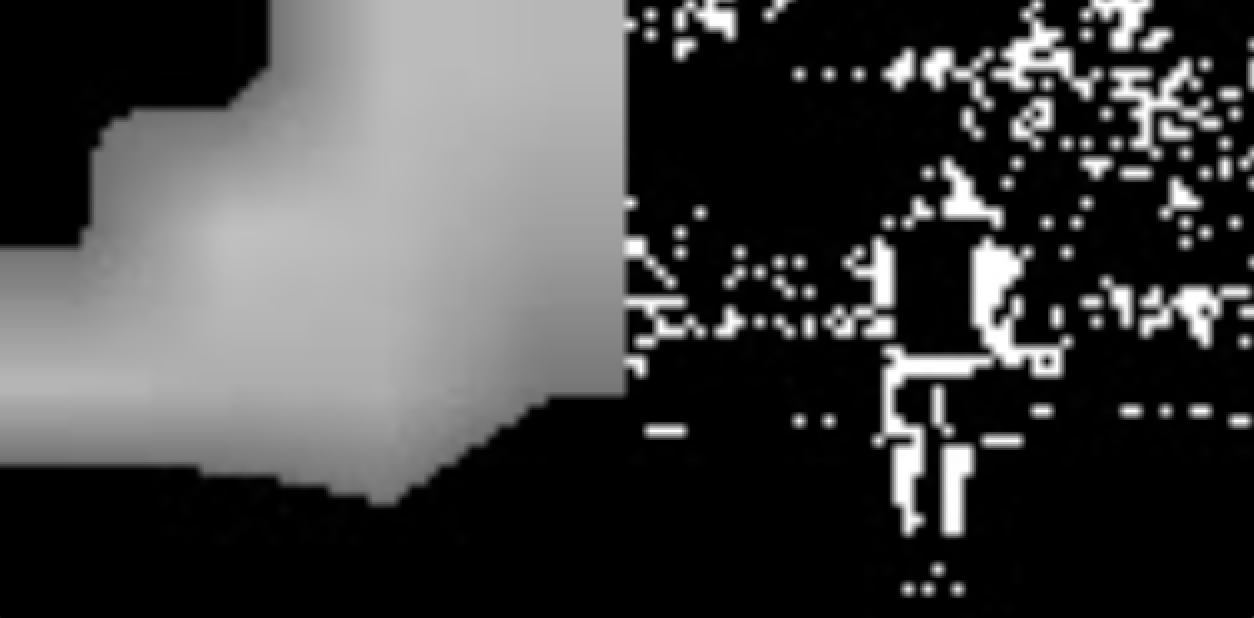
\includegraphics[width=50mm]{images/cam/radio.png}
        & 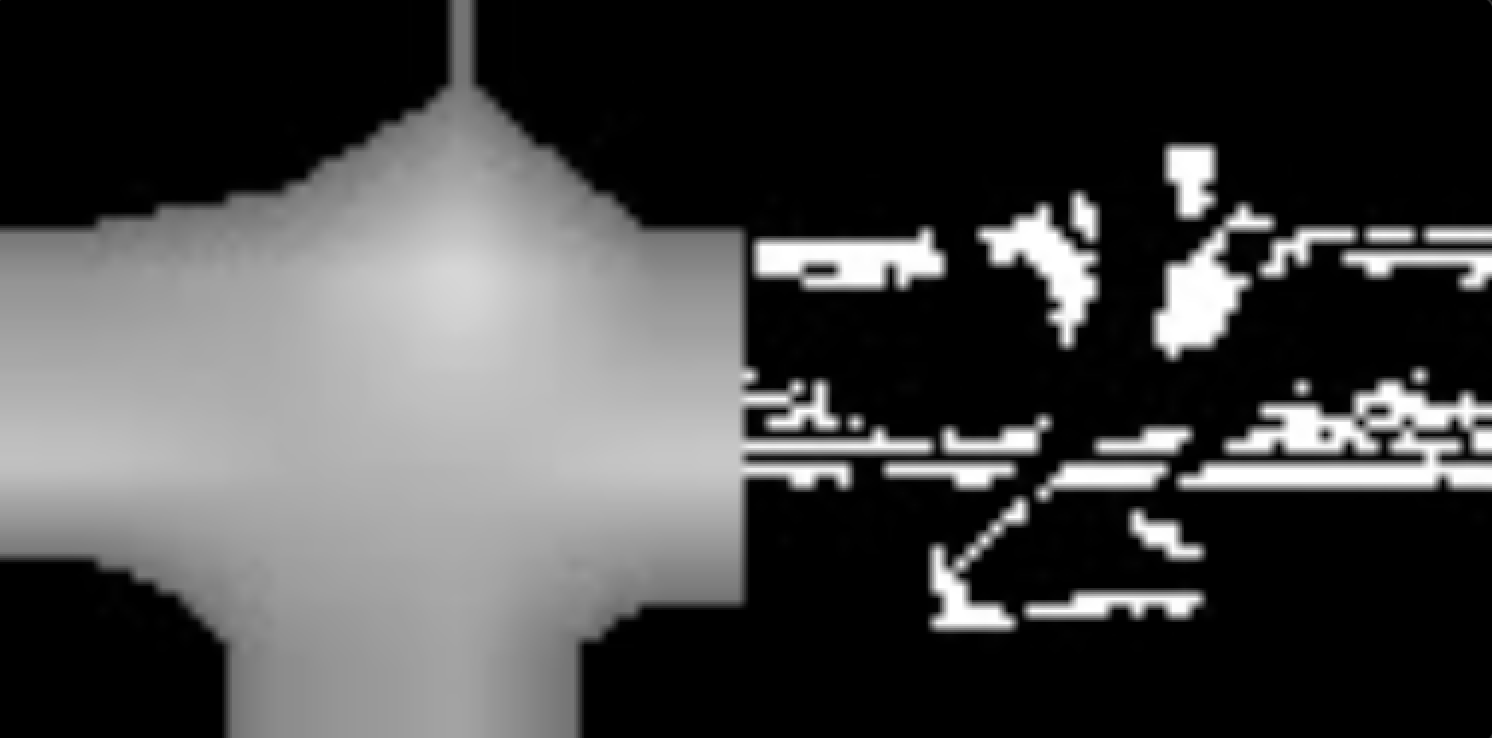
\includegraphics[width=50mm]{images/cam/running.png}
      \\ \hline
    \end{tabular}
  \end{center}
  \caption{観測された動画特徴例}
  \label{examples}
\end{table}

このようにして出力されたGrad Camの動画と二値化動画を横に繋ぎ合わせ,どのような特徴があるか
観察した.すると表\ref{examples}のような特徴を観測した.
ここで判断根拠分布は
\begin{enumerate}
  \item 優美なダンスは画面「下部」に「広く」分布している \\
        領域を大きく使っていることから手足を頻繁に使う
  \item 普通のダンスは画面「中部」に「小さく」分布している \\
        領域を狭く使っていることから体幹移動を頻繁に使う
  \item その他の動作は画面「上部」に「広く」分布している \\
        判断根拠が離散している
\end{enumerate}
という仮説を立てた.この仮説を検証するため,それぞれの動画に対して
縦に三つに分割した時の判断根拠分布率を算出した.
\clearpage

\begin{figure}[t]
  \begin{center}
    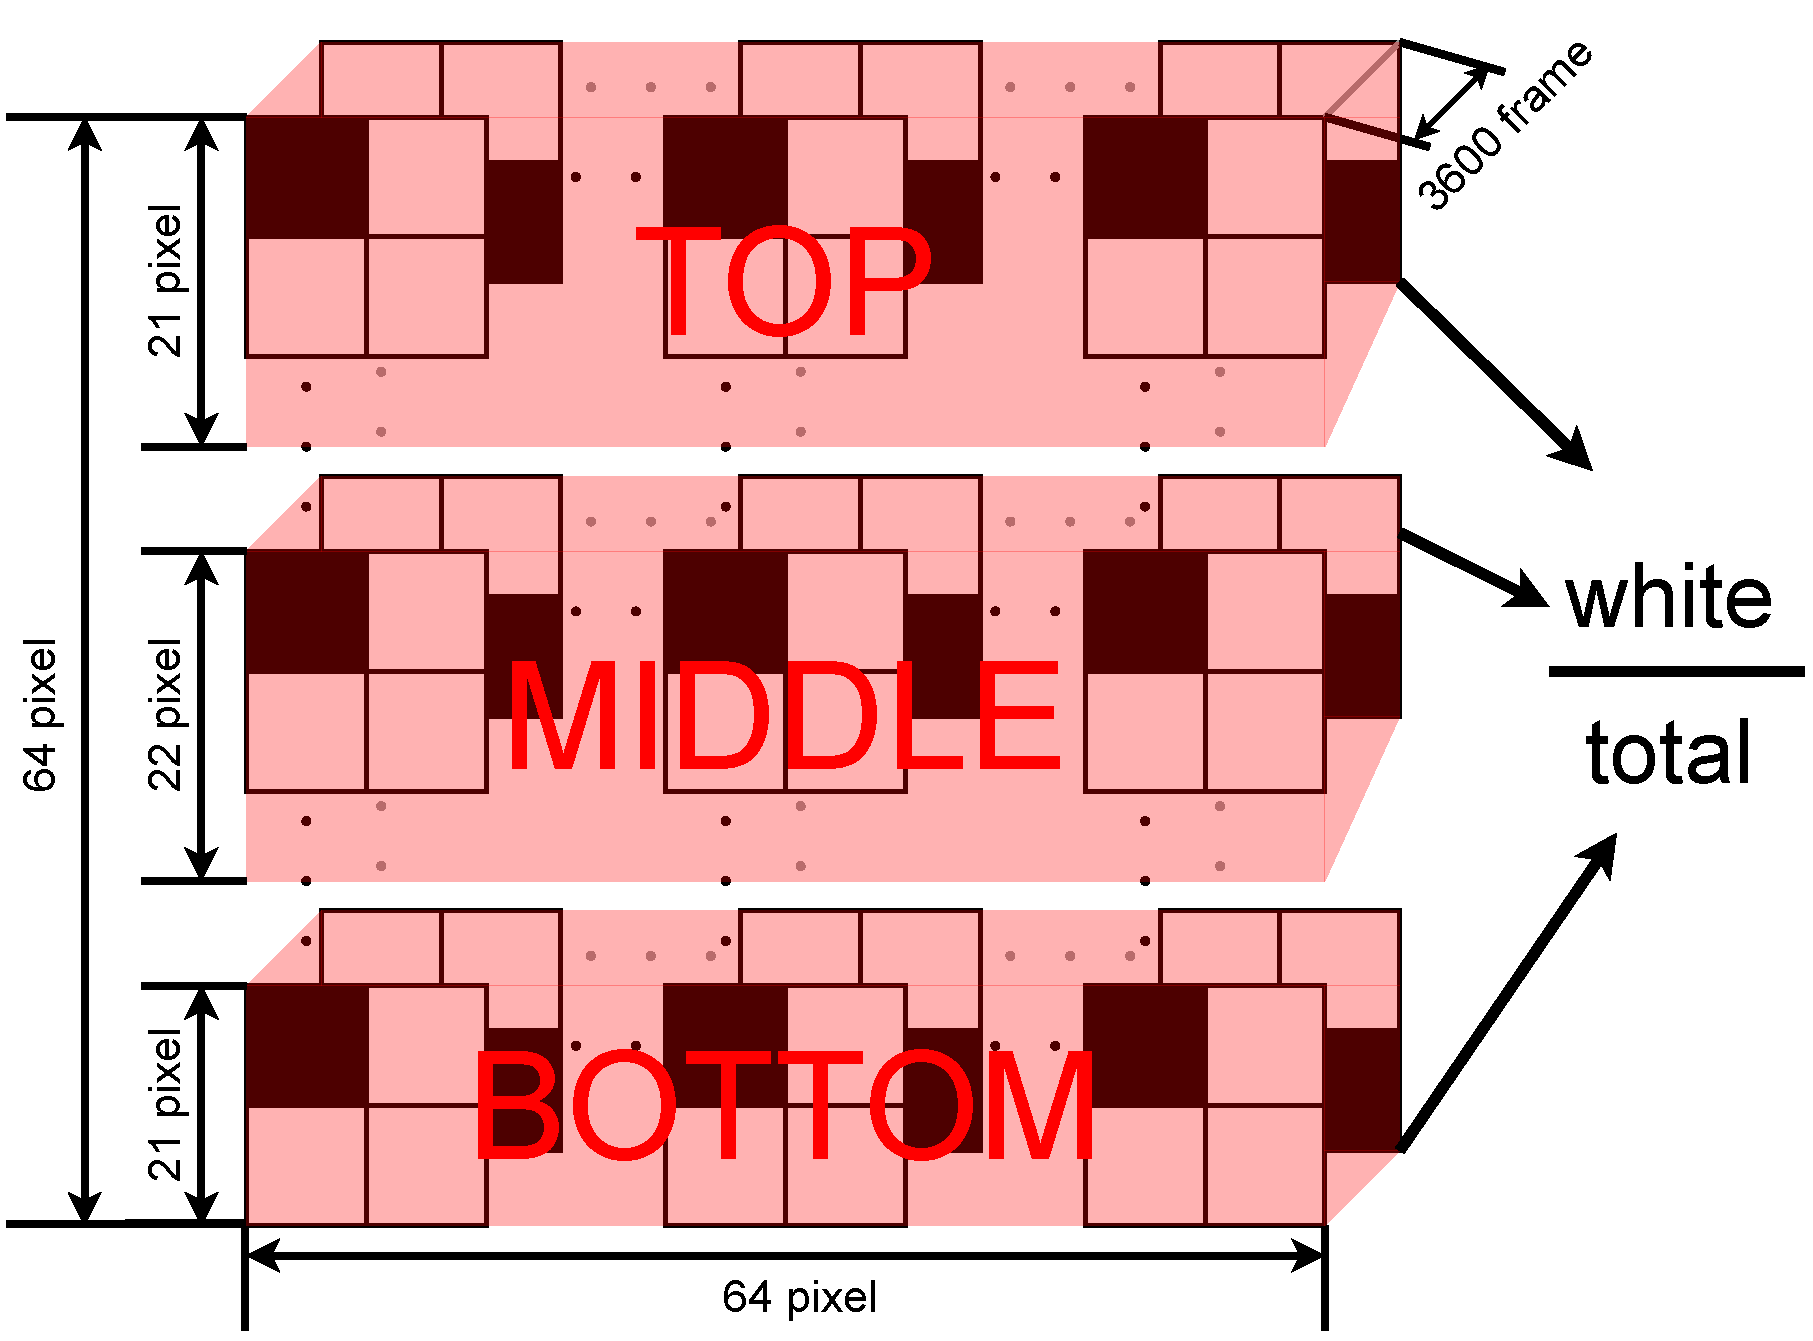
\includegraphics[width=120mm]{images/chart/divide.pdf}
  \end{center}
  \caption{Grad Cam動画の画素計算方法}
  \label{divide_graph}
\end{figure}

図\ref{divide_graph}のようにGrad Cam動画データを縦に三分割した.
黒画素以外の個数を数え,それを指定領域数で割ることでその領域に占める
判断根拠の分布率を算出した.

その結果,表\ref{devide_summary}のような数値を得た.いくつかの動画について,
優美なダンスでは「中部」「下部」に広く分布していることが分かった.
いくつかの動画では,領域を大きく使っていることから
手足を頻繁に使う動作が優美と判定されているように思う.
逆に,普通のダンスはいくつかの動画では分布が狭い,つまり画面中央に密集しており,
体幹移動を頻繁に使うのではないかと考える.
しかし,入力データに複数人で踊っているデータが存在していたり,精度の悪い動画や
先の仮説にそぐわない動画も存在しているので相関は薄く推測の域は出ない.

\begin{table}[t]
  \begin{center}
    \begin{tabular}{|c|p{5mm}p{5mm}p{5mm}|p{5mm}p{5mm}p{5mm}|p{5mm}p{5mm}p{5mm}|p{5mm}p{5mm}p{5mm}|} \hline
        & \multicolumn{6}{|c|}{学習用} & \multicolumn{6}{|c|}{推論用} \\ \cline{2-13}
        &上 &中 &下 &上 &中 &下 &上 &中 &下 &上 &中 &下 \\ \hline
        &2.1 &34.4 &62.8 &10.8 &16.9 &48.8 &0.0 &43.2 &38.2 &40.6 &71.2 &72.4 \\
        & \multicolumn{3}{|c|}{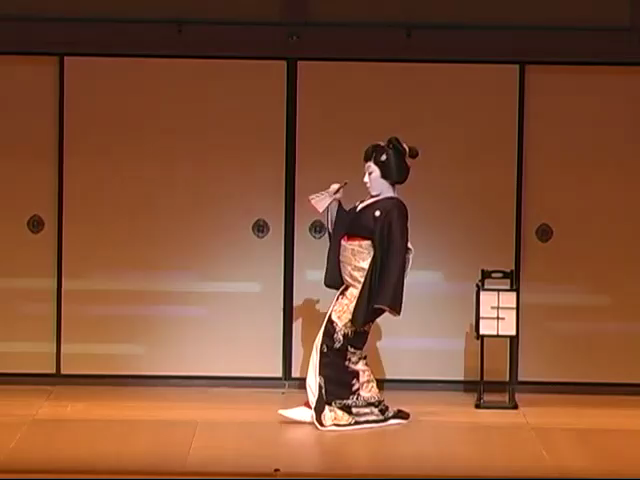
\includegraphics[width=18mm]{images/snaps/japanese_elegant.png}}
        & \multicolumn{3}{|c|}{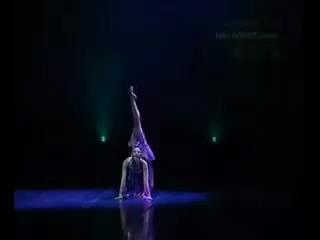
\includegraphics[width=18mm]{images/snaps/chinese_elegant.png}}
        & \multicolumn{3}{|c|}{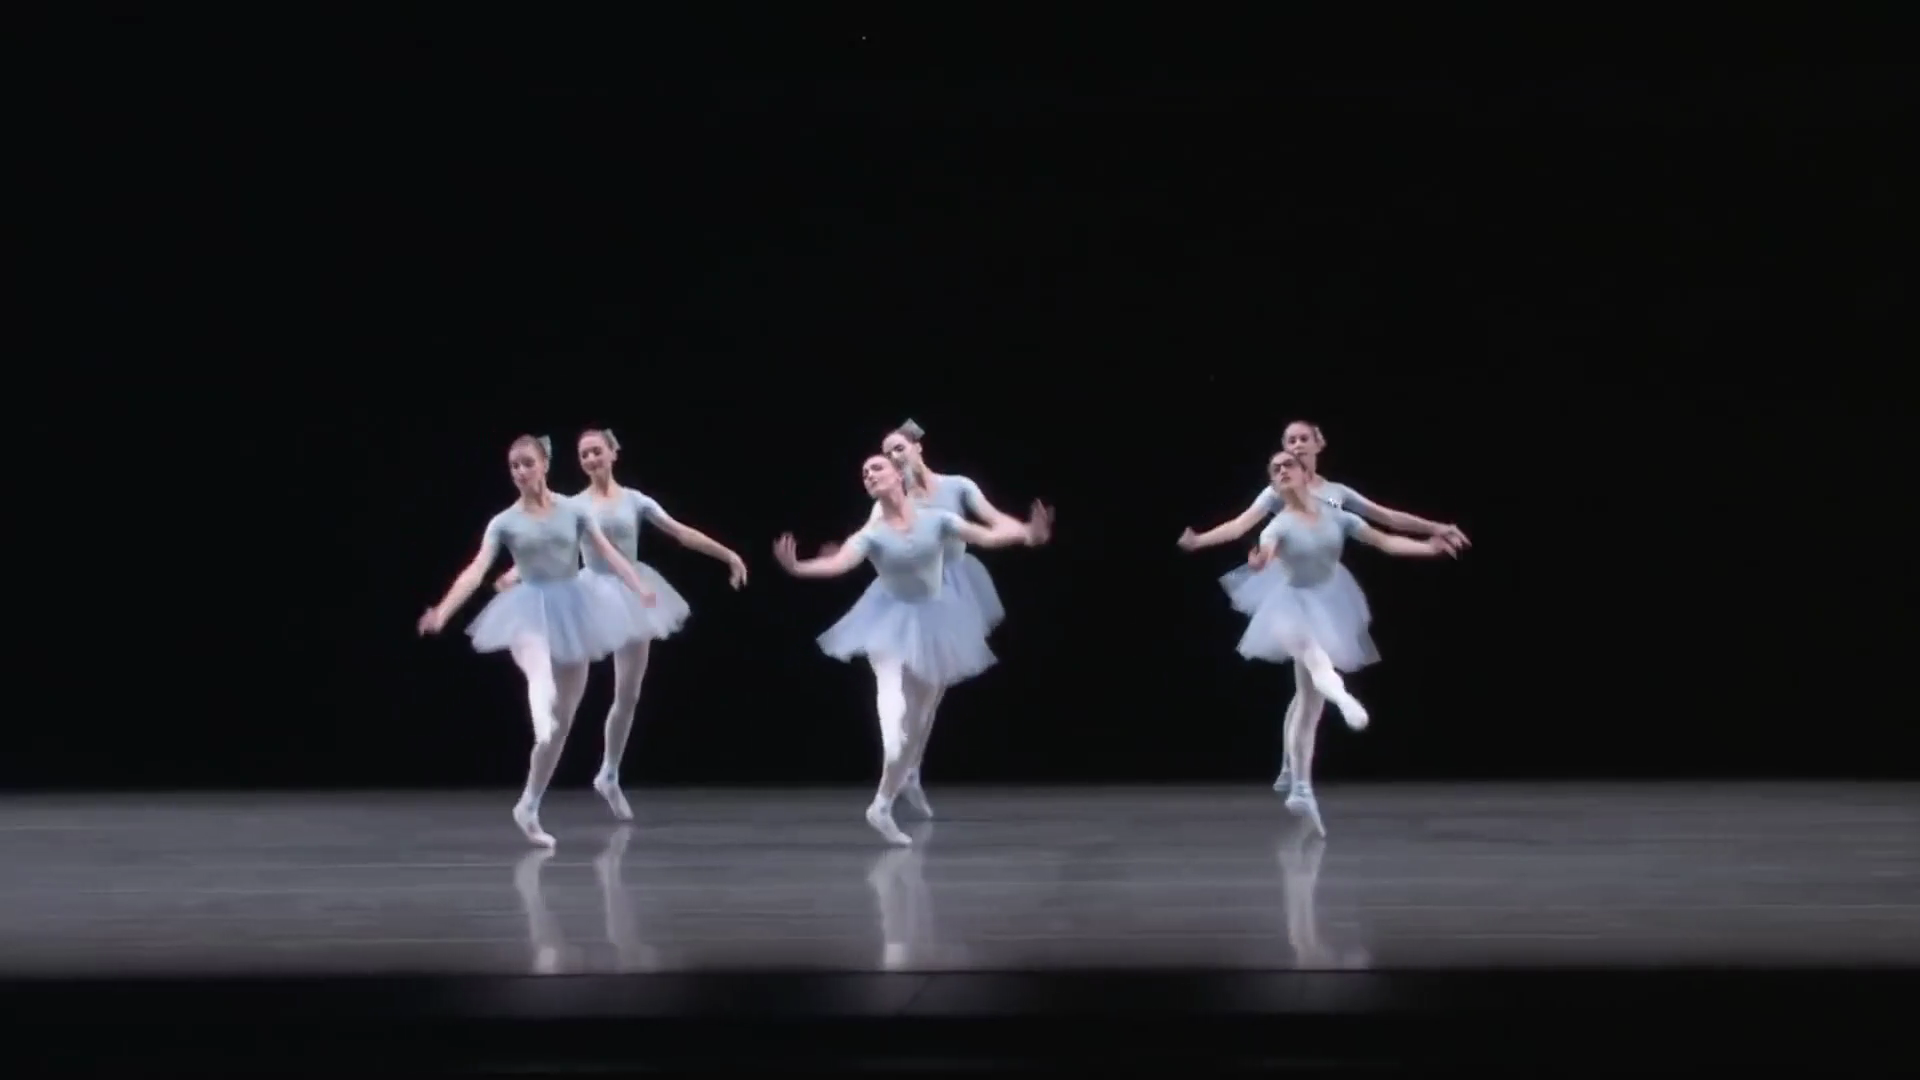
\includegraphics[width=18mm]{images/snaps/ballet_group_elegant.png}}
        & \multicolumn{3}{|c|}{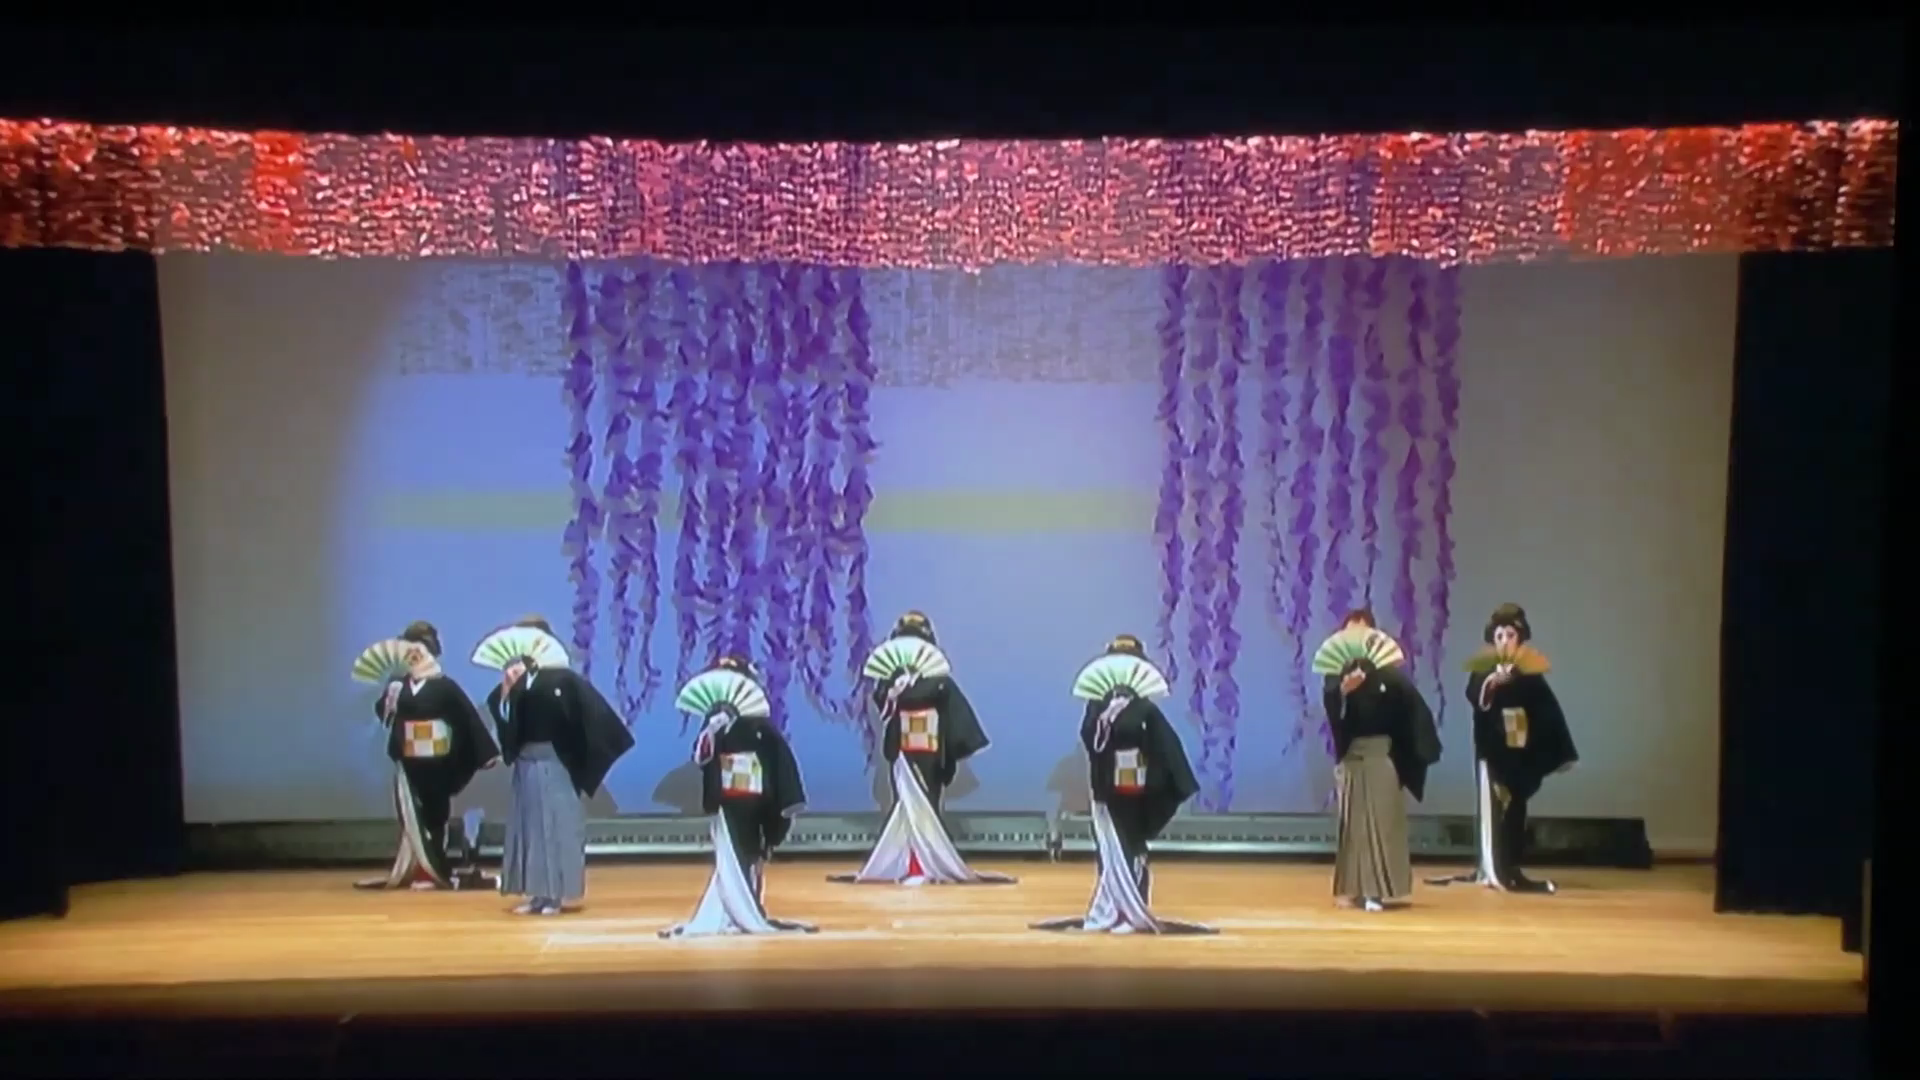
\includegraphics[width=18mm]{images/snaps/japanese_group_elegant.png}}
      \\ \cline{2-13}
      優美
        &6.8 &60.0 &31.4 &48.3 &71.6 &33.8 &1.3 &48.1 &54.7 &6.3 &28.5 &52.1 \\
        & \multicolumn{3}{|c|}{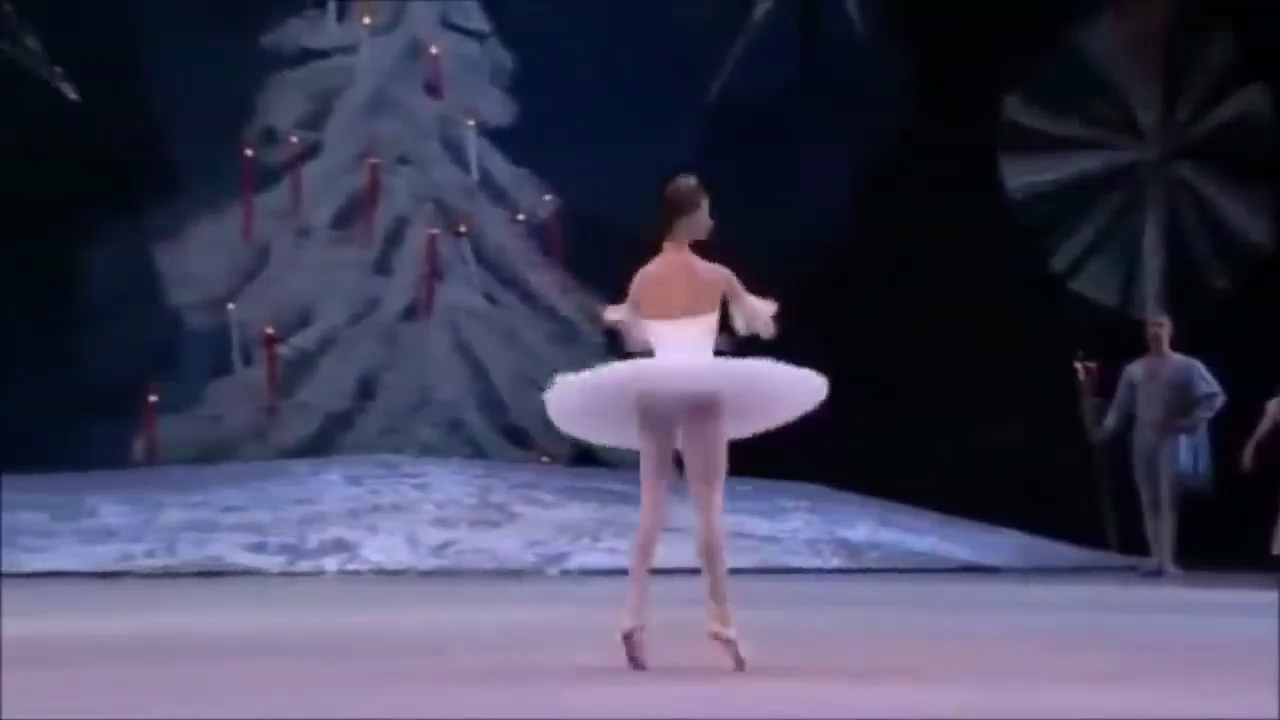
\includegraphics[width=18mm]{images/snaps/ballet_elegant.png}}
        & \multicolumn{3}{|c|}{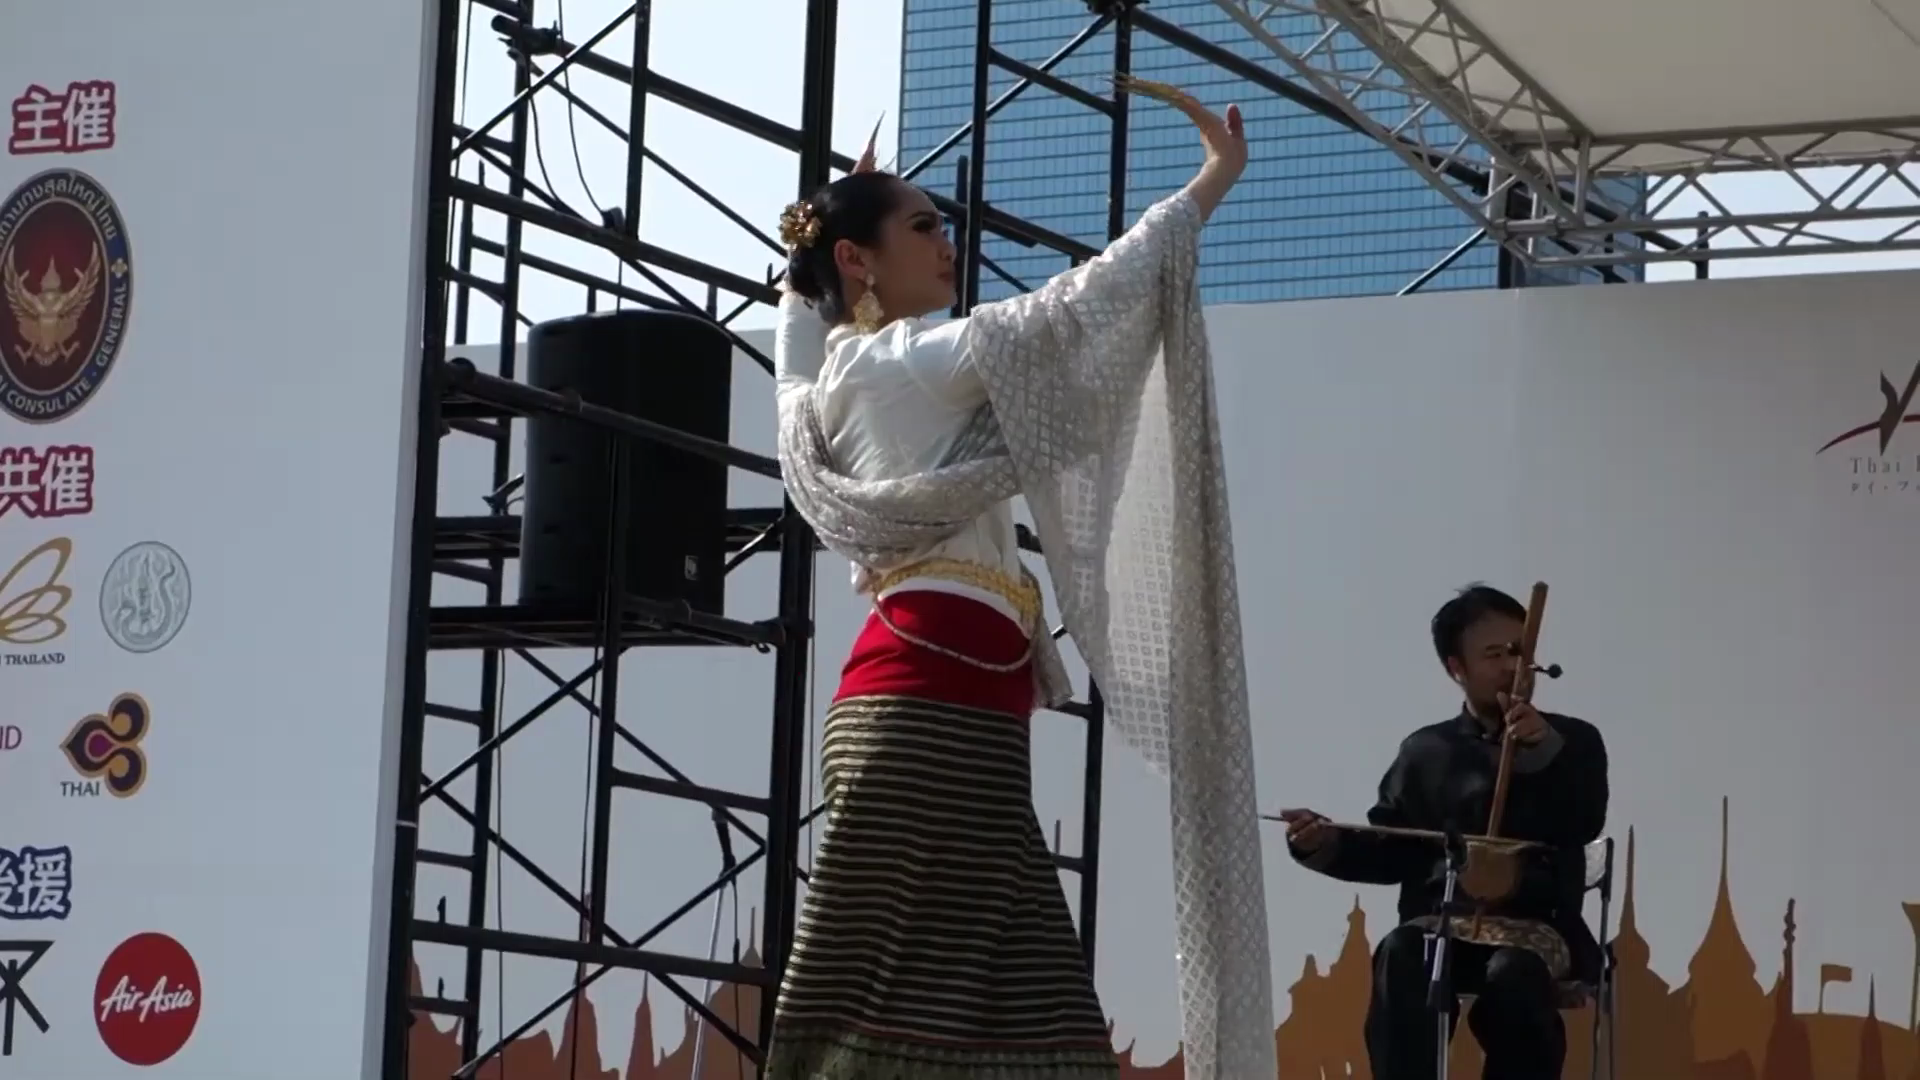
\includegraphics[width=18mm]{images/snaps/thai_elegant.png}}
        & \multicolumn{3}{|c|}{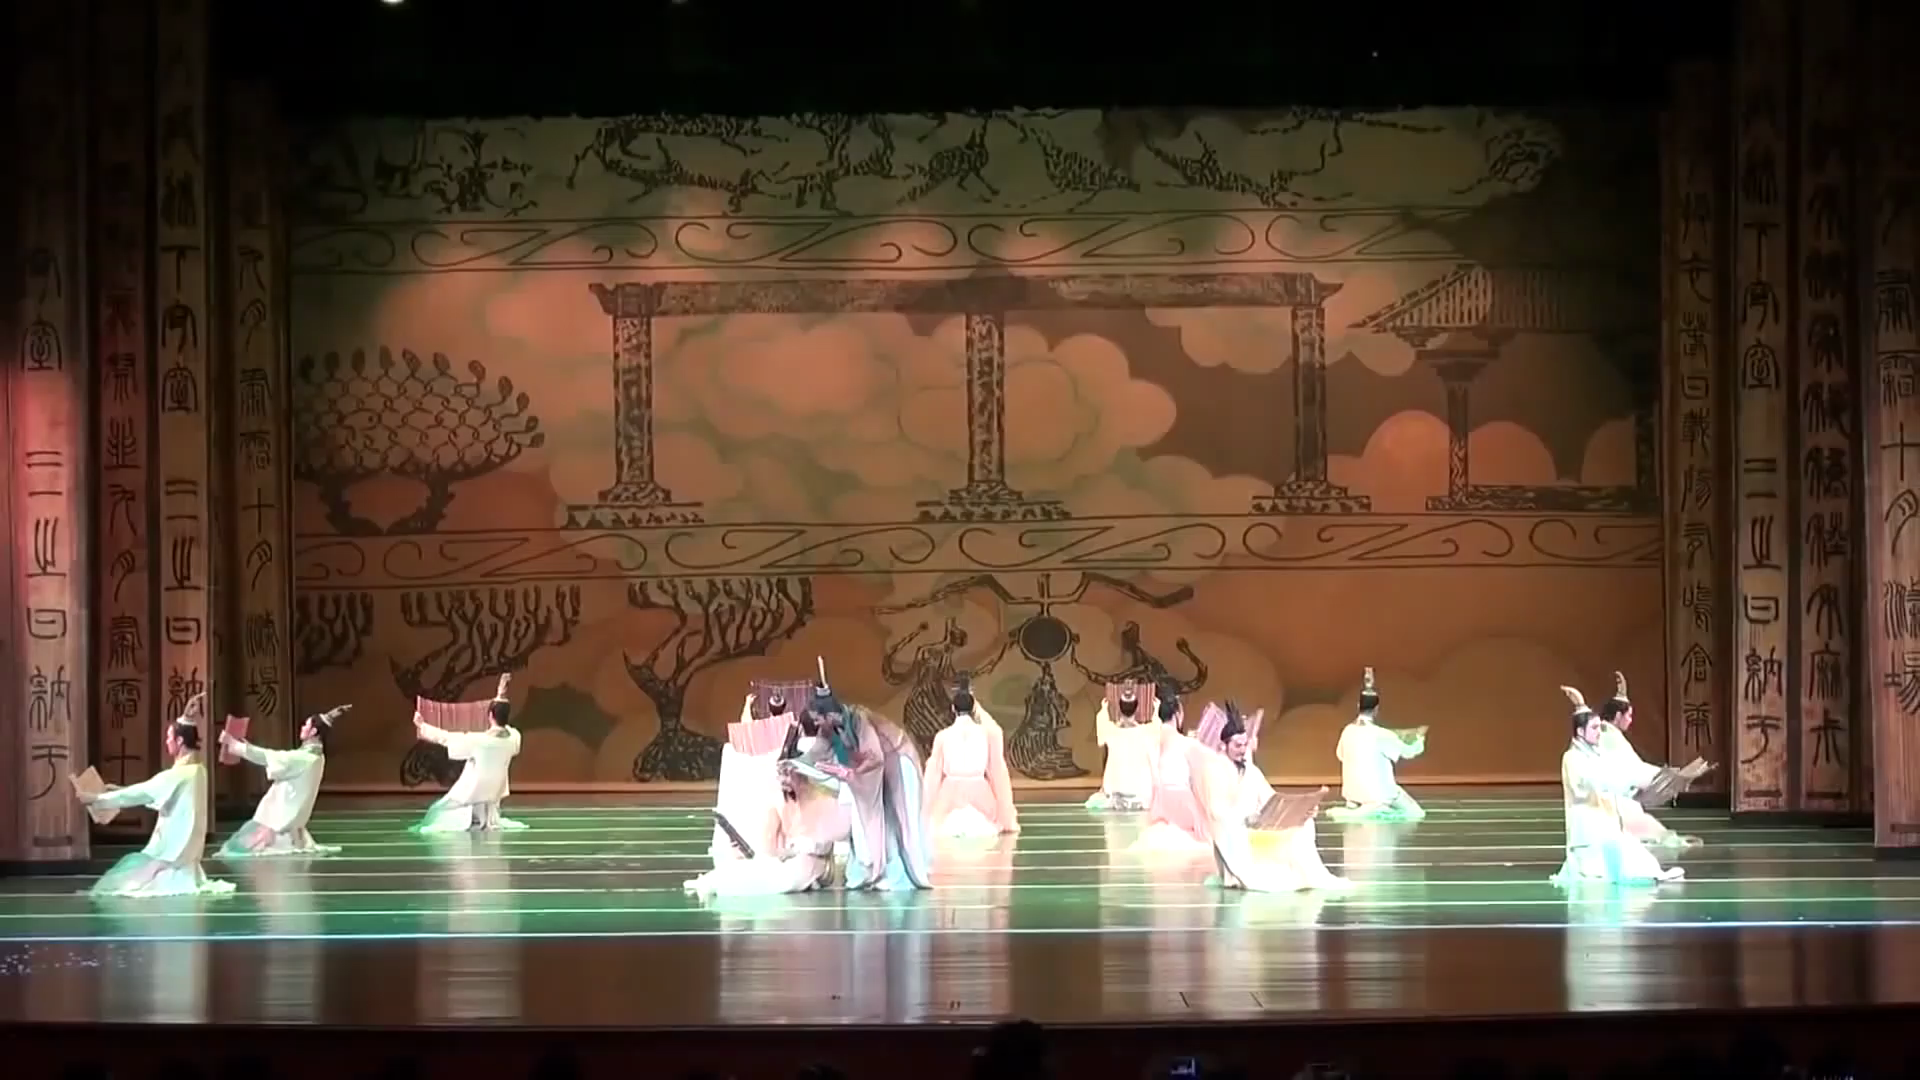
\includegraphics[width=18mm]{images/snaps/chinese_group_elegant.png}}
        & \multicolumn{3}{|c|}{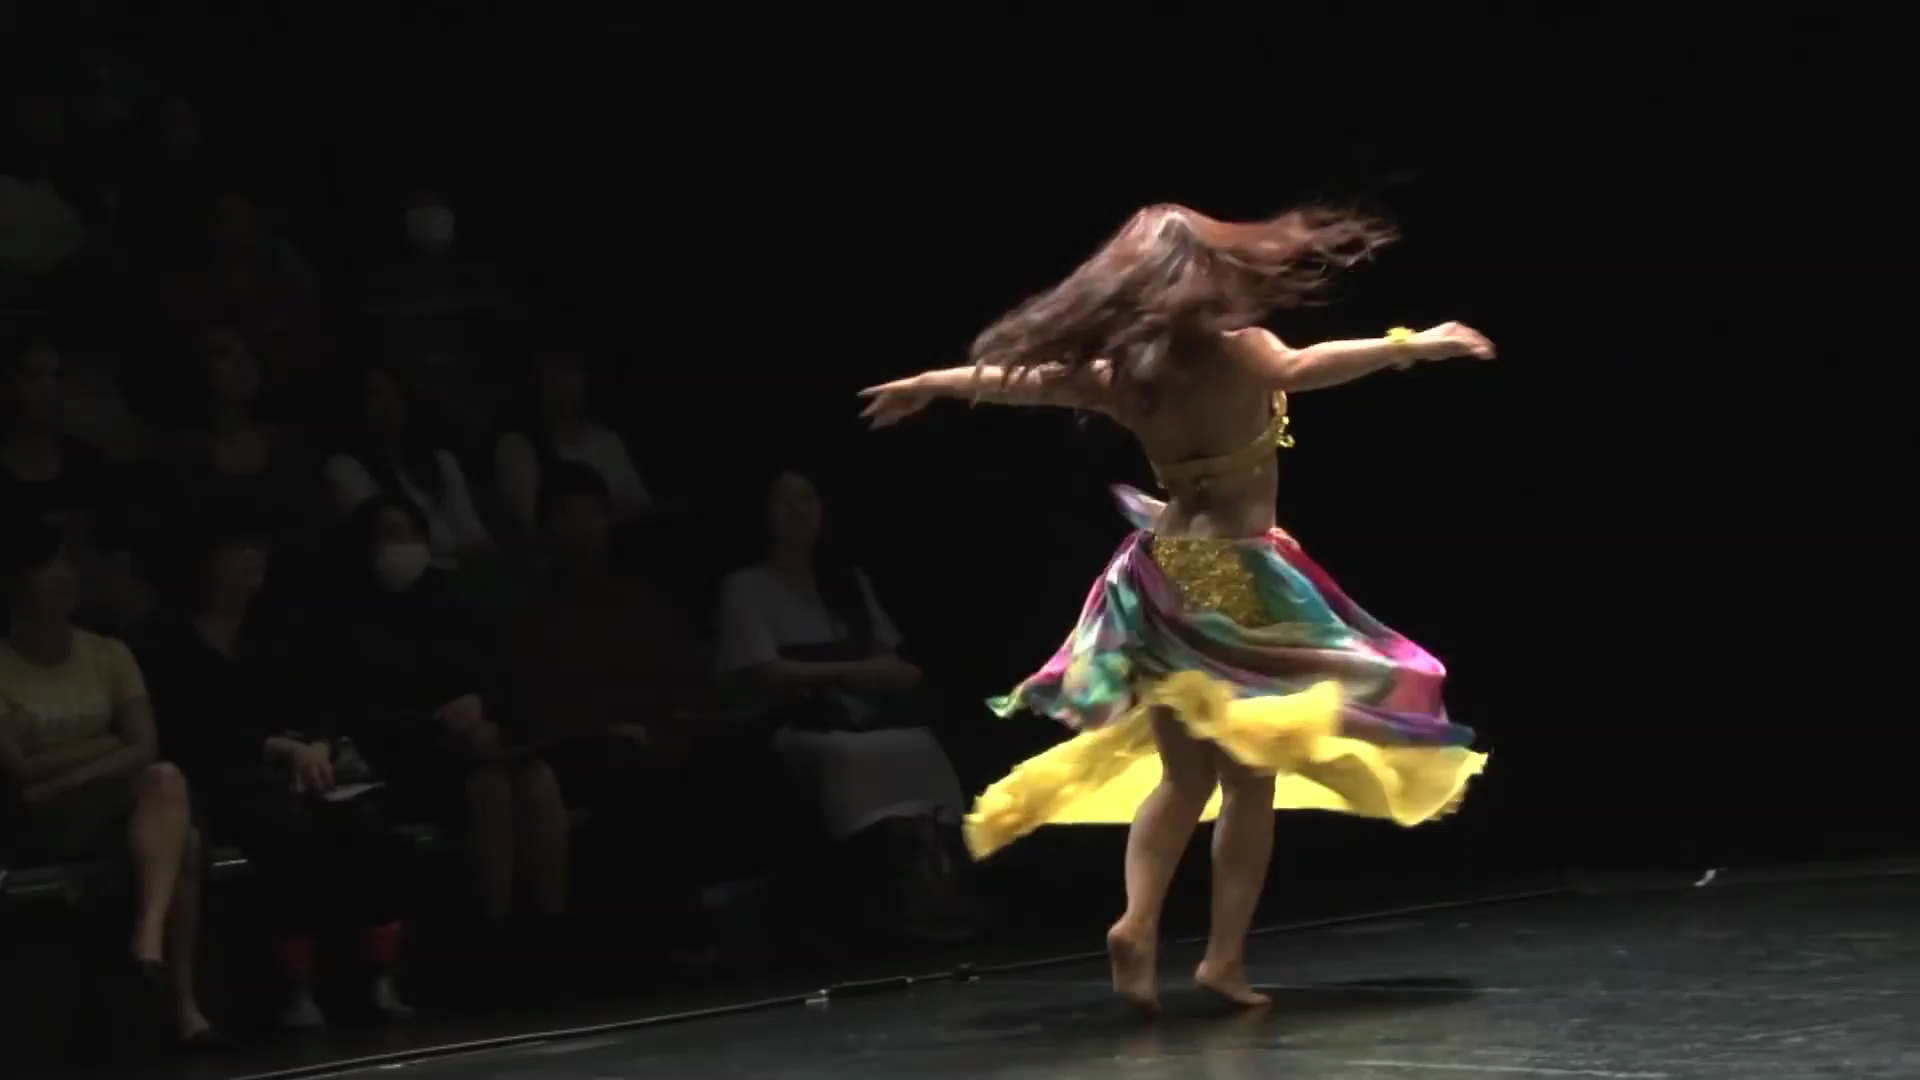
\includegraphics[width=18mm]{images/snaps/belly_elegant.png}}
      \\ \cline{2-13}
        &28.0 &11.7 &24.7 & & & & & & & & & \\
        & \multicolumn{3}{|c|}{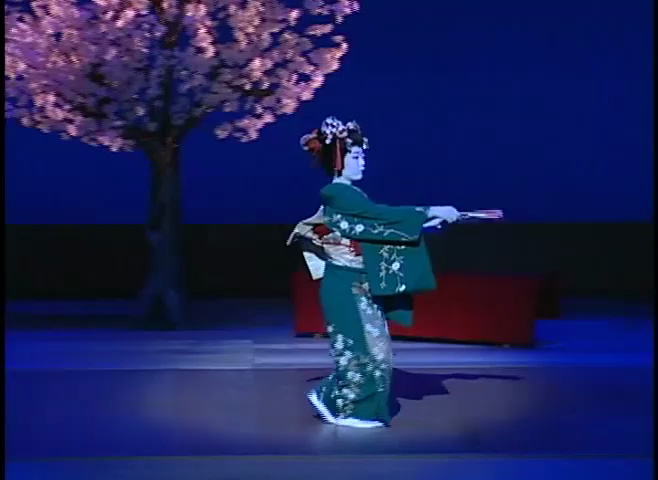
\includegraphics[width=18mm]{images/snaps/japanese2_elegant.png}}
        & \multicolumn{3}{|c|}{}
        & \multicolumn{3}{|c|}{}
        & \multicolumn{3}{|c|}{}
      \\ \hline
        &16.0 &42.5 &36.6 &21.4 &32.0 &27.4 &79.8 &72.9 &59.5 &13.8 &75.5 &22.4 \\
        & \multicolumn{3}{|c|}{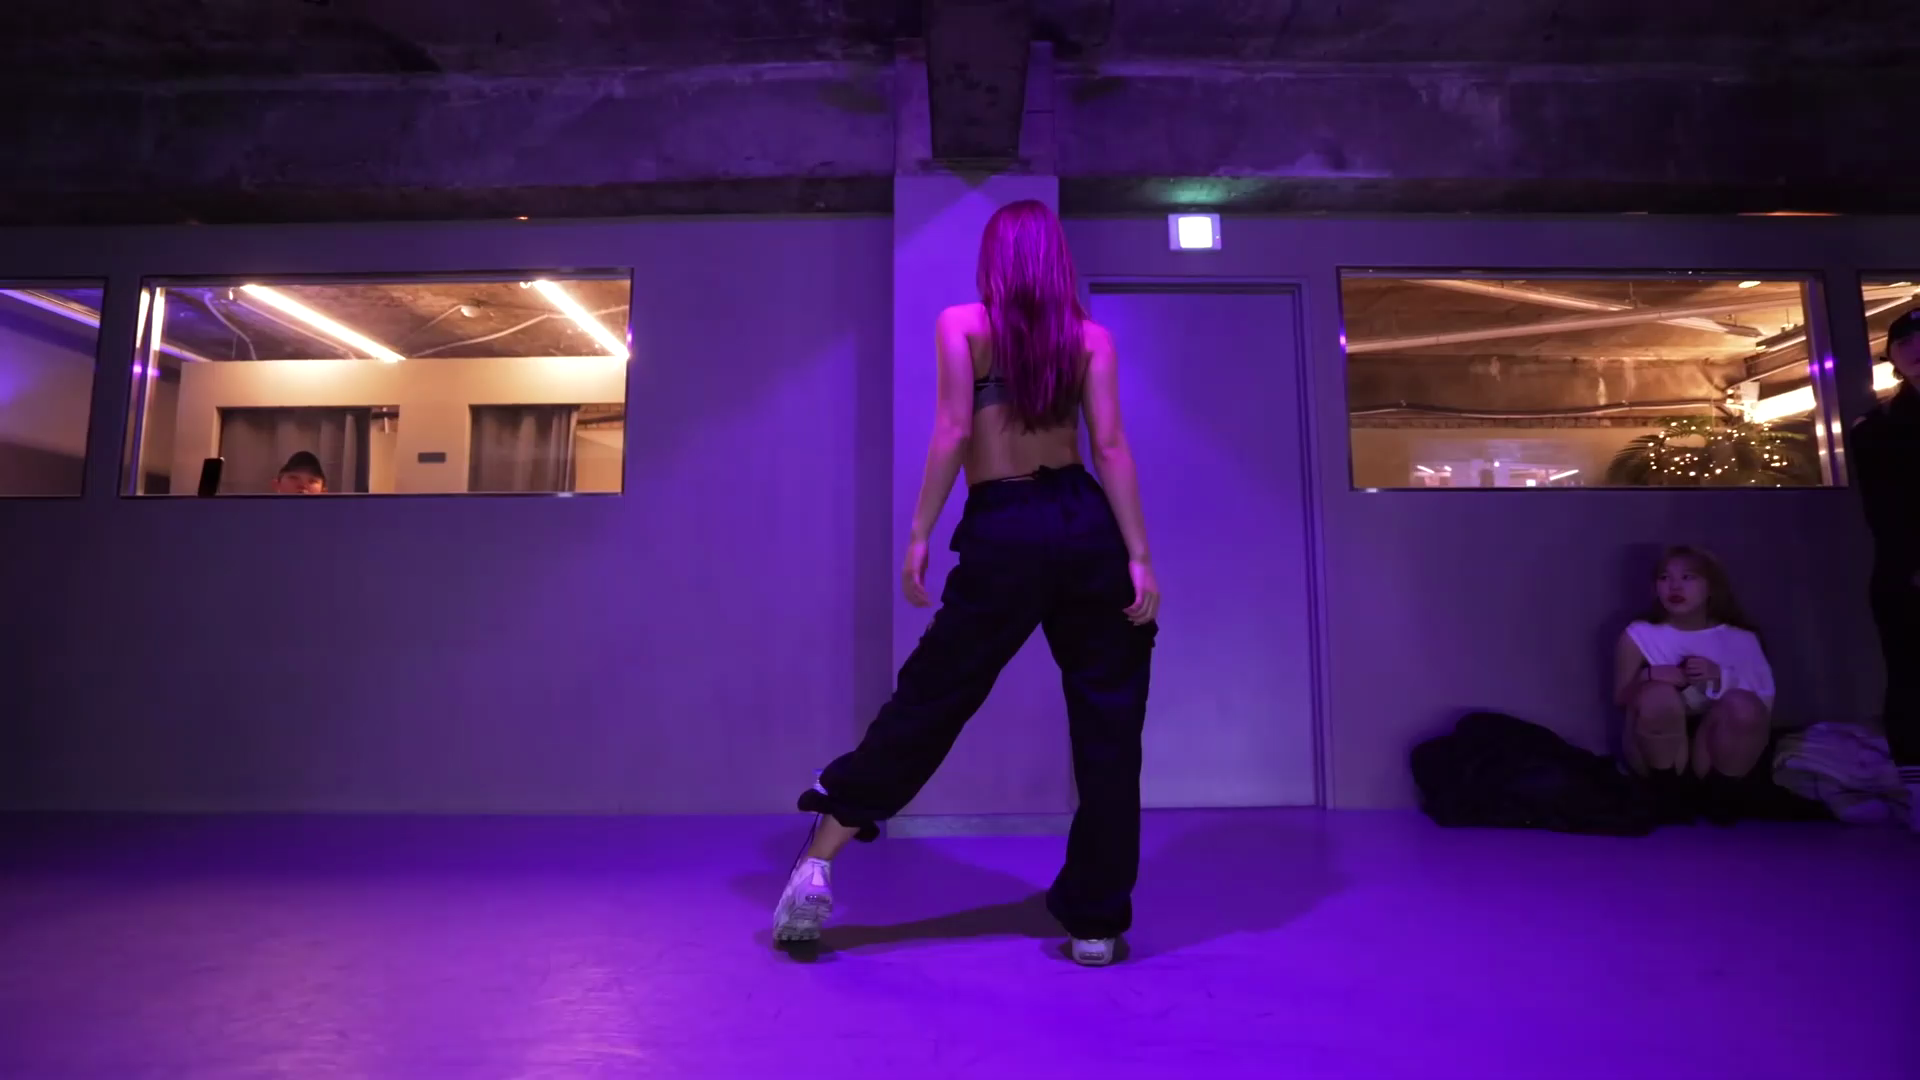
\includegraphics[width=18mm]{images/snaps/ariana_dance.png}}
        & \multicolumn{3}{|c|}{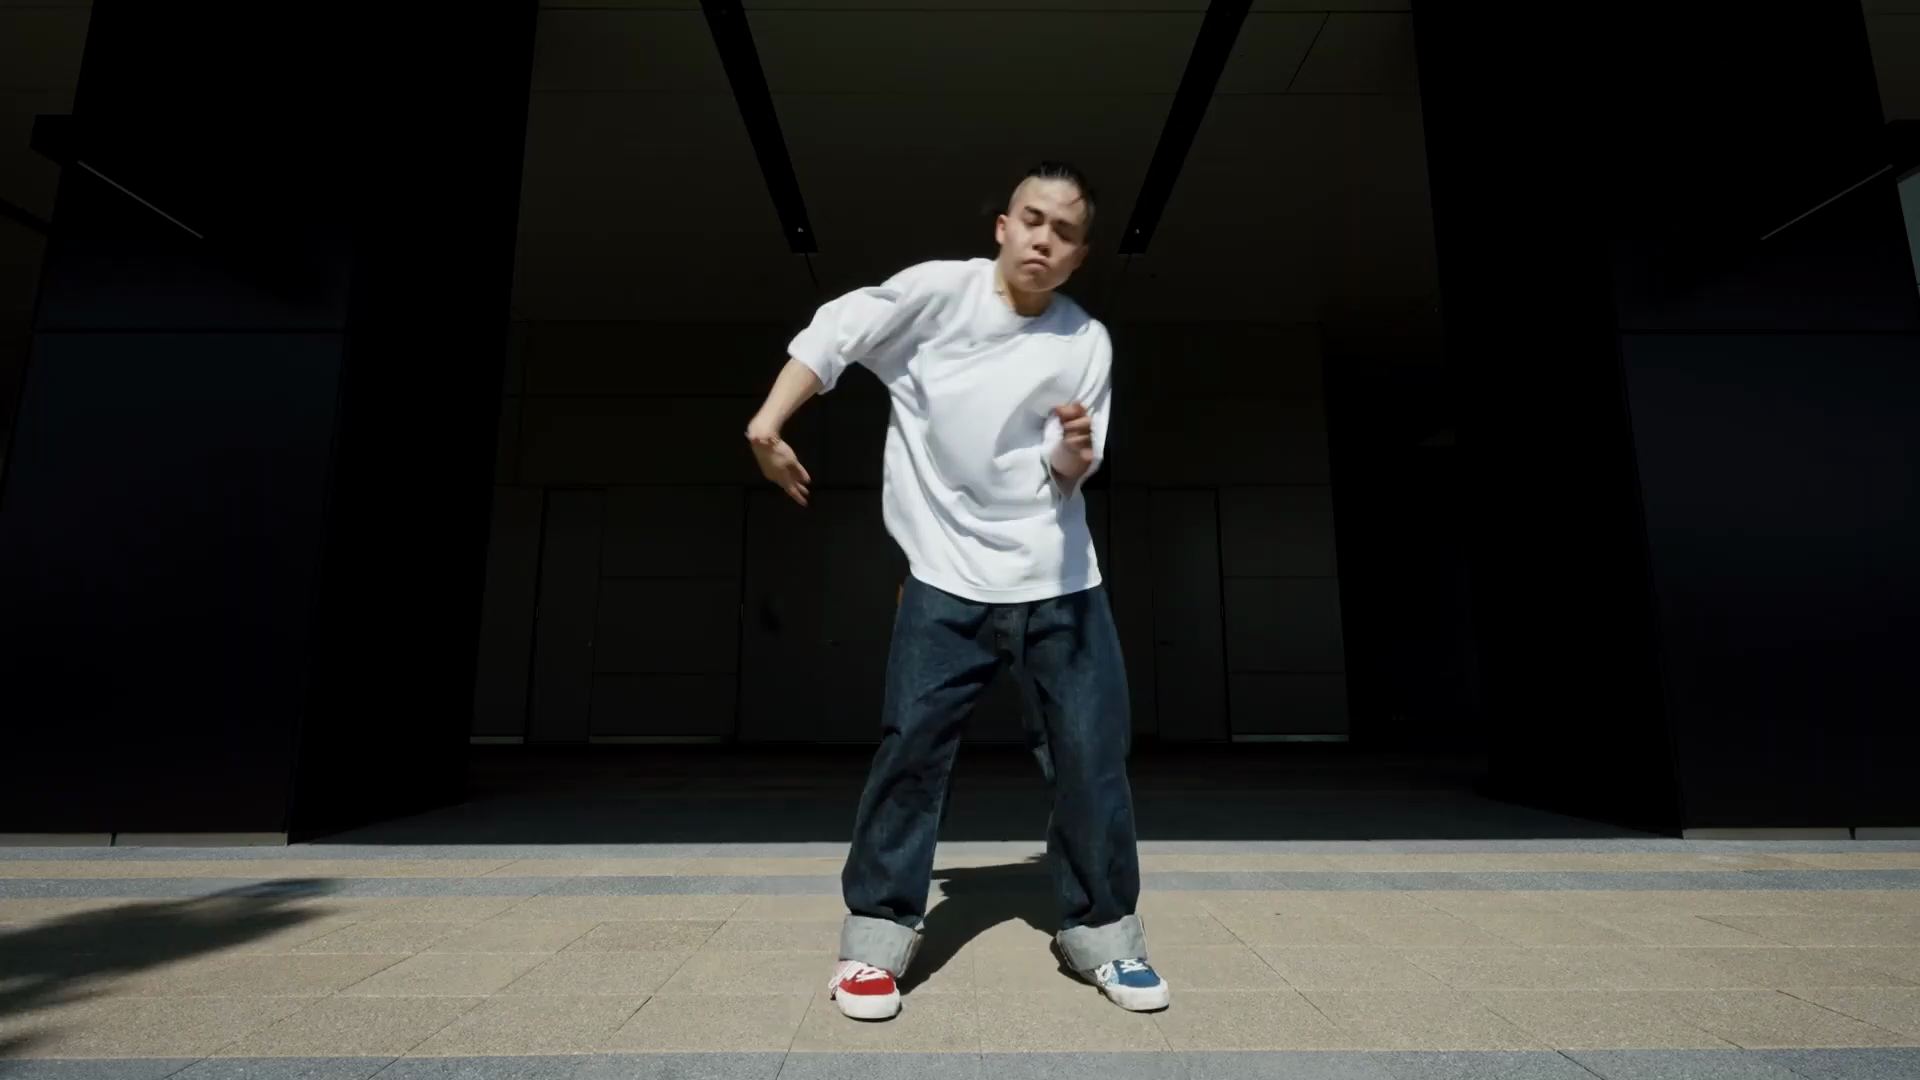
\includegraphics[width=18mm]{images/snaps/kadokawa_dream_dance.png}}
        & \multicolumn{3}{|c|}{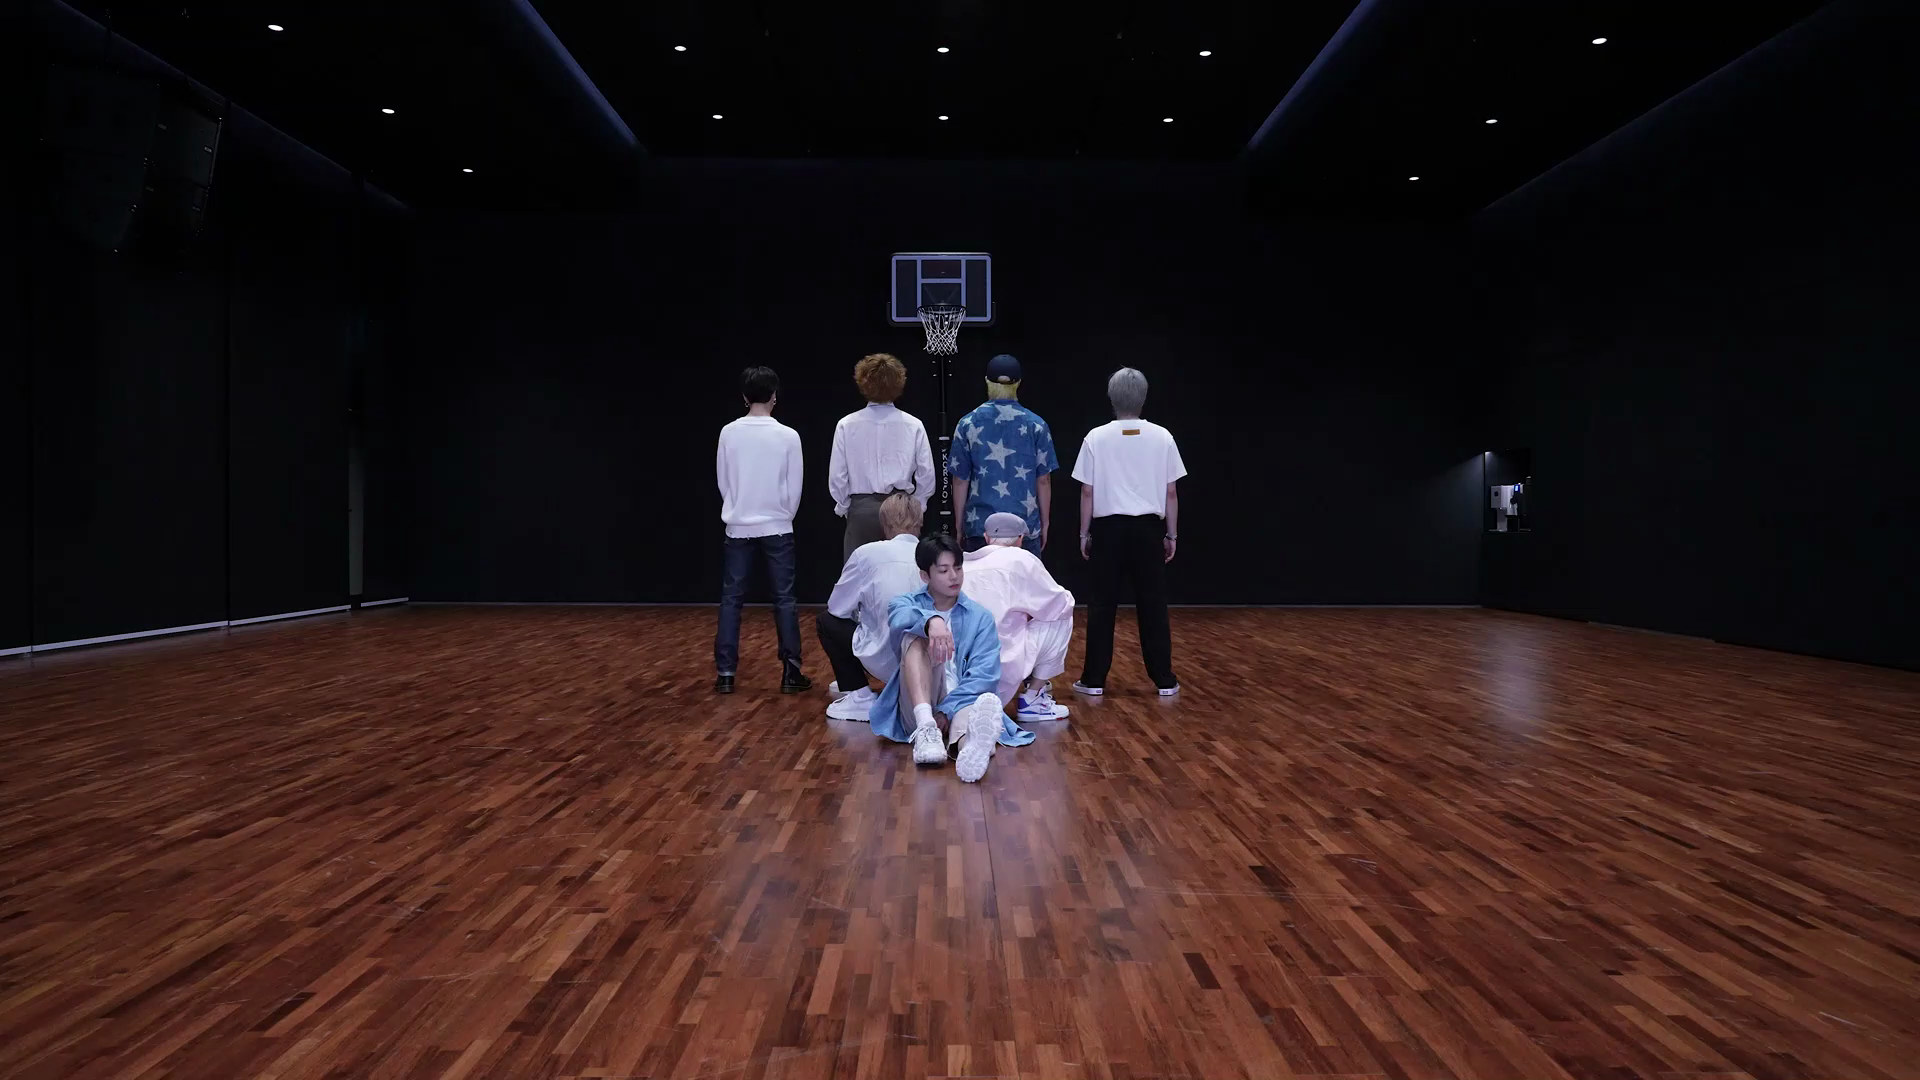
\includegraphics[width=18mm]{images/snaps/bts_group_dance.png}}
        & \multicolumn{3}{|c|}{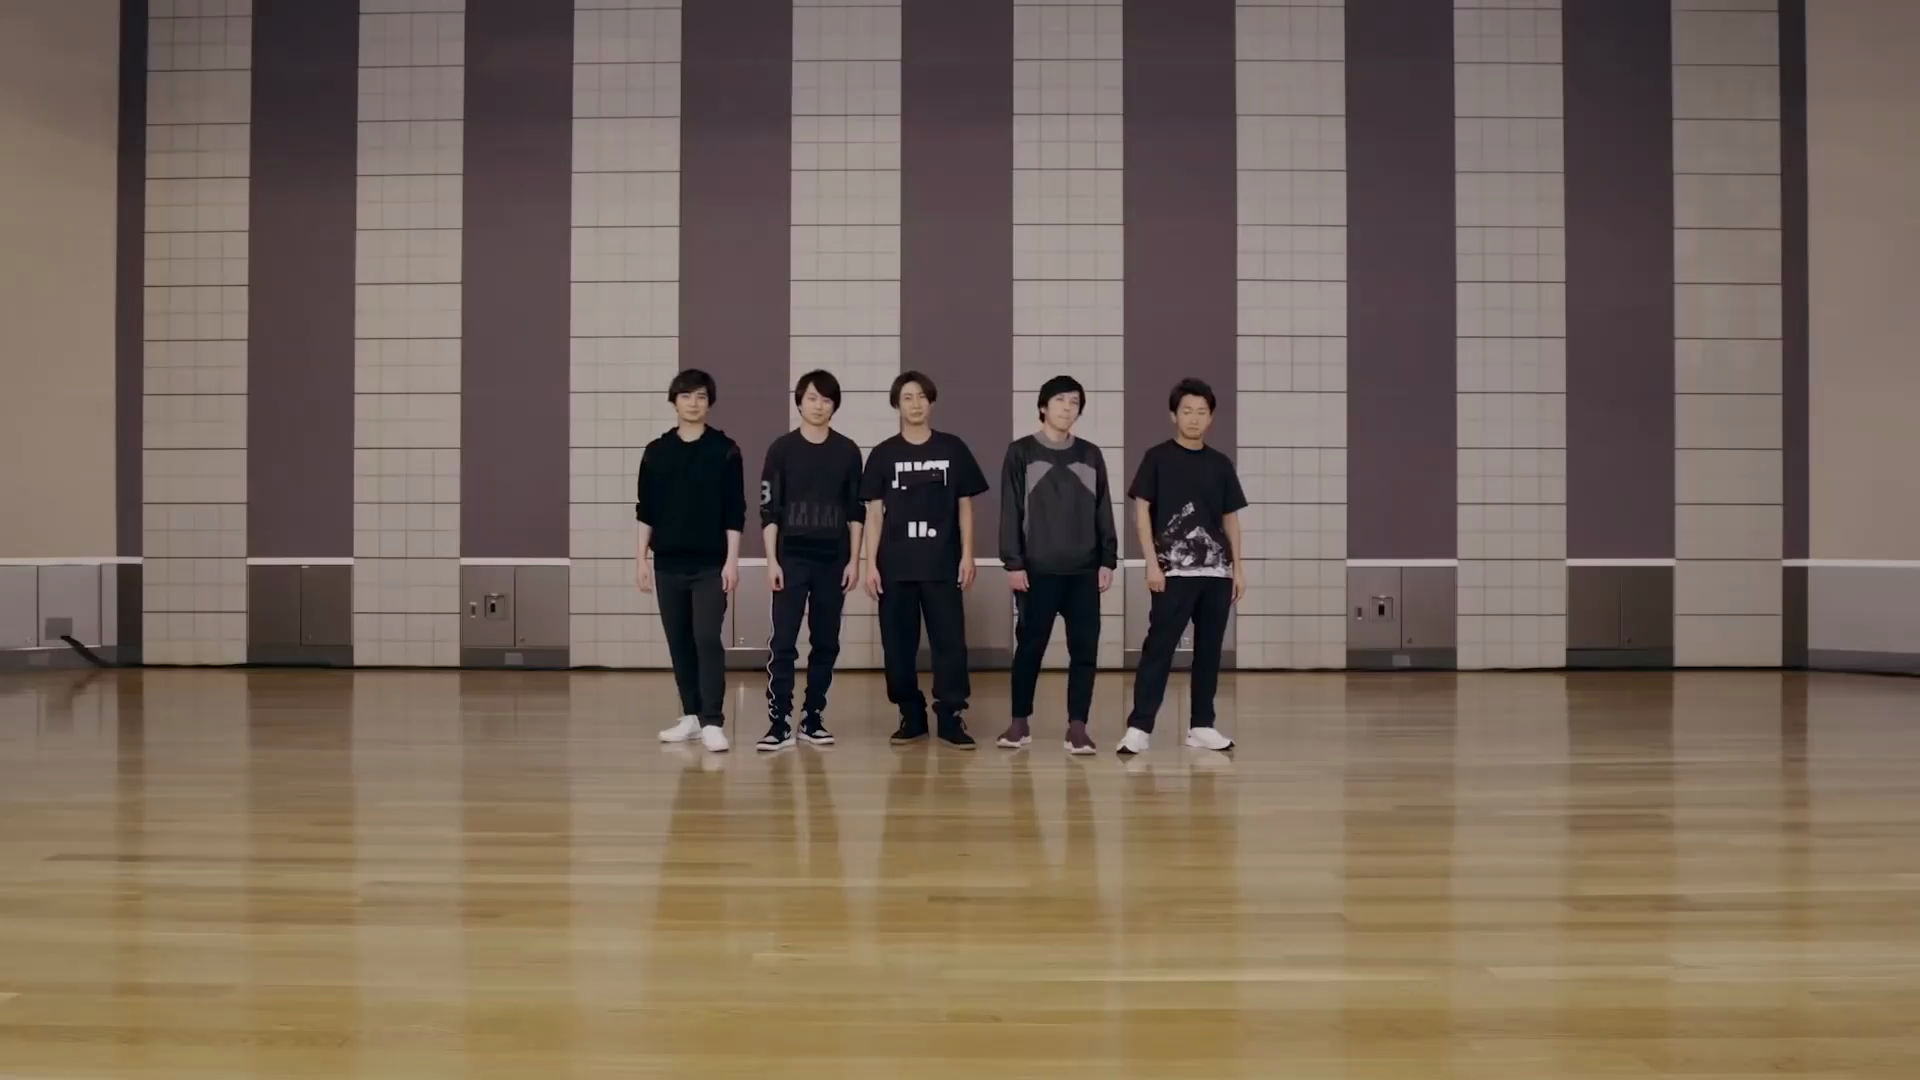
\includegraphics[width=18mm]{images/snaps/arashi_group_dance.png}}
      \\ \cline{2-13}
      普通
        &11.4 &38.4 &13.6 &31.6 &47.9 &50.3 &12.5 &26.2 &4.8 &15.4 &8.3 &22.4 \\
        & \multicolumn{3}{|c|}{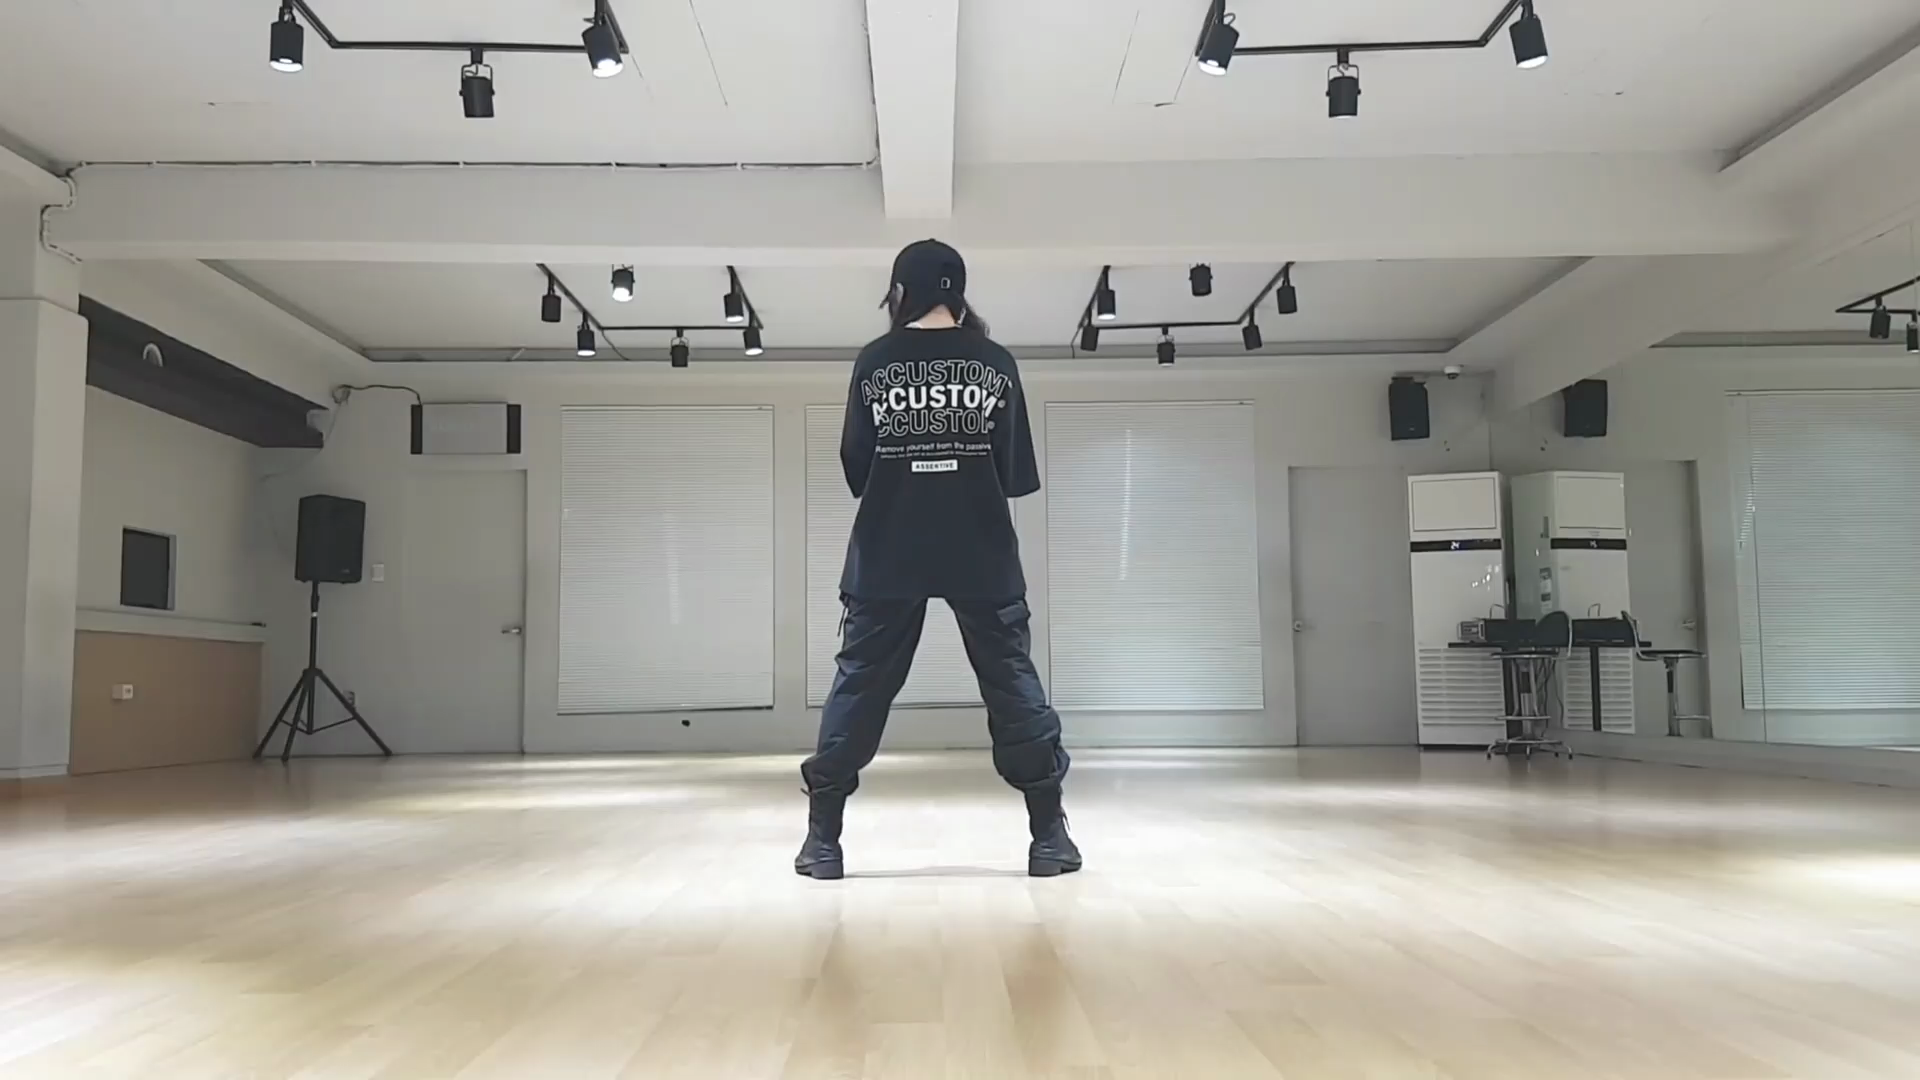
\includegraphics[width=18mm]{images/snaps/bts_dance.png}}
        & \multicolumn{3}{|c|}{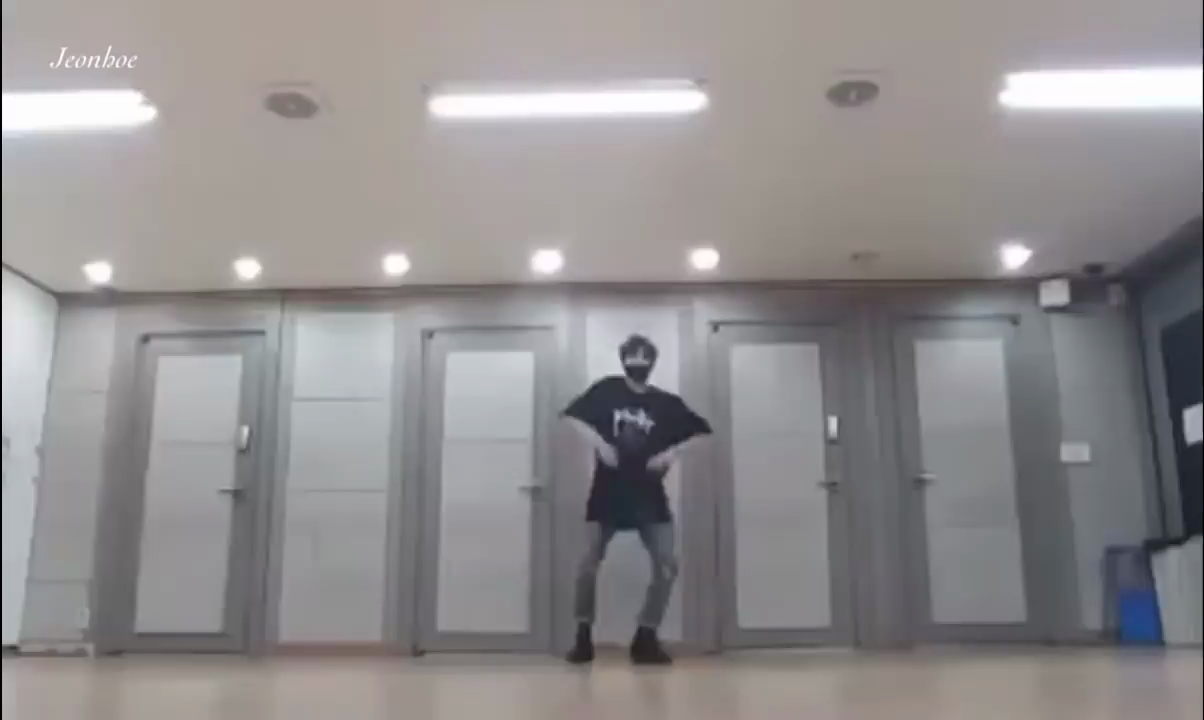
\includegraphics[width=18mm]{images/snaps/manolo_dance.png}}
        & \multicolumn{3}{|c|}{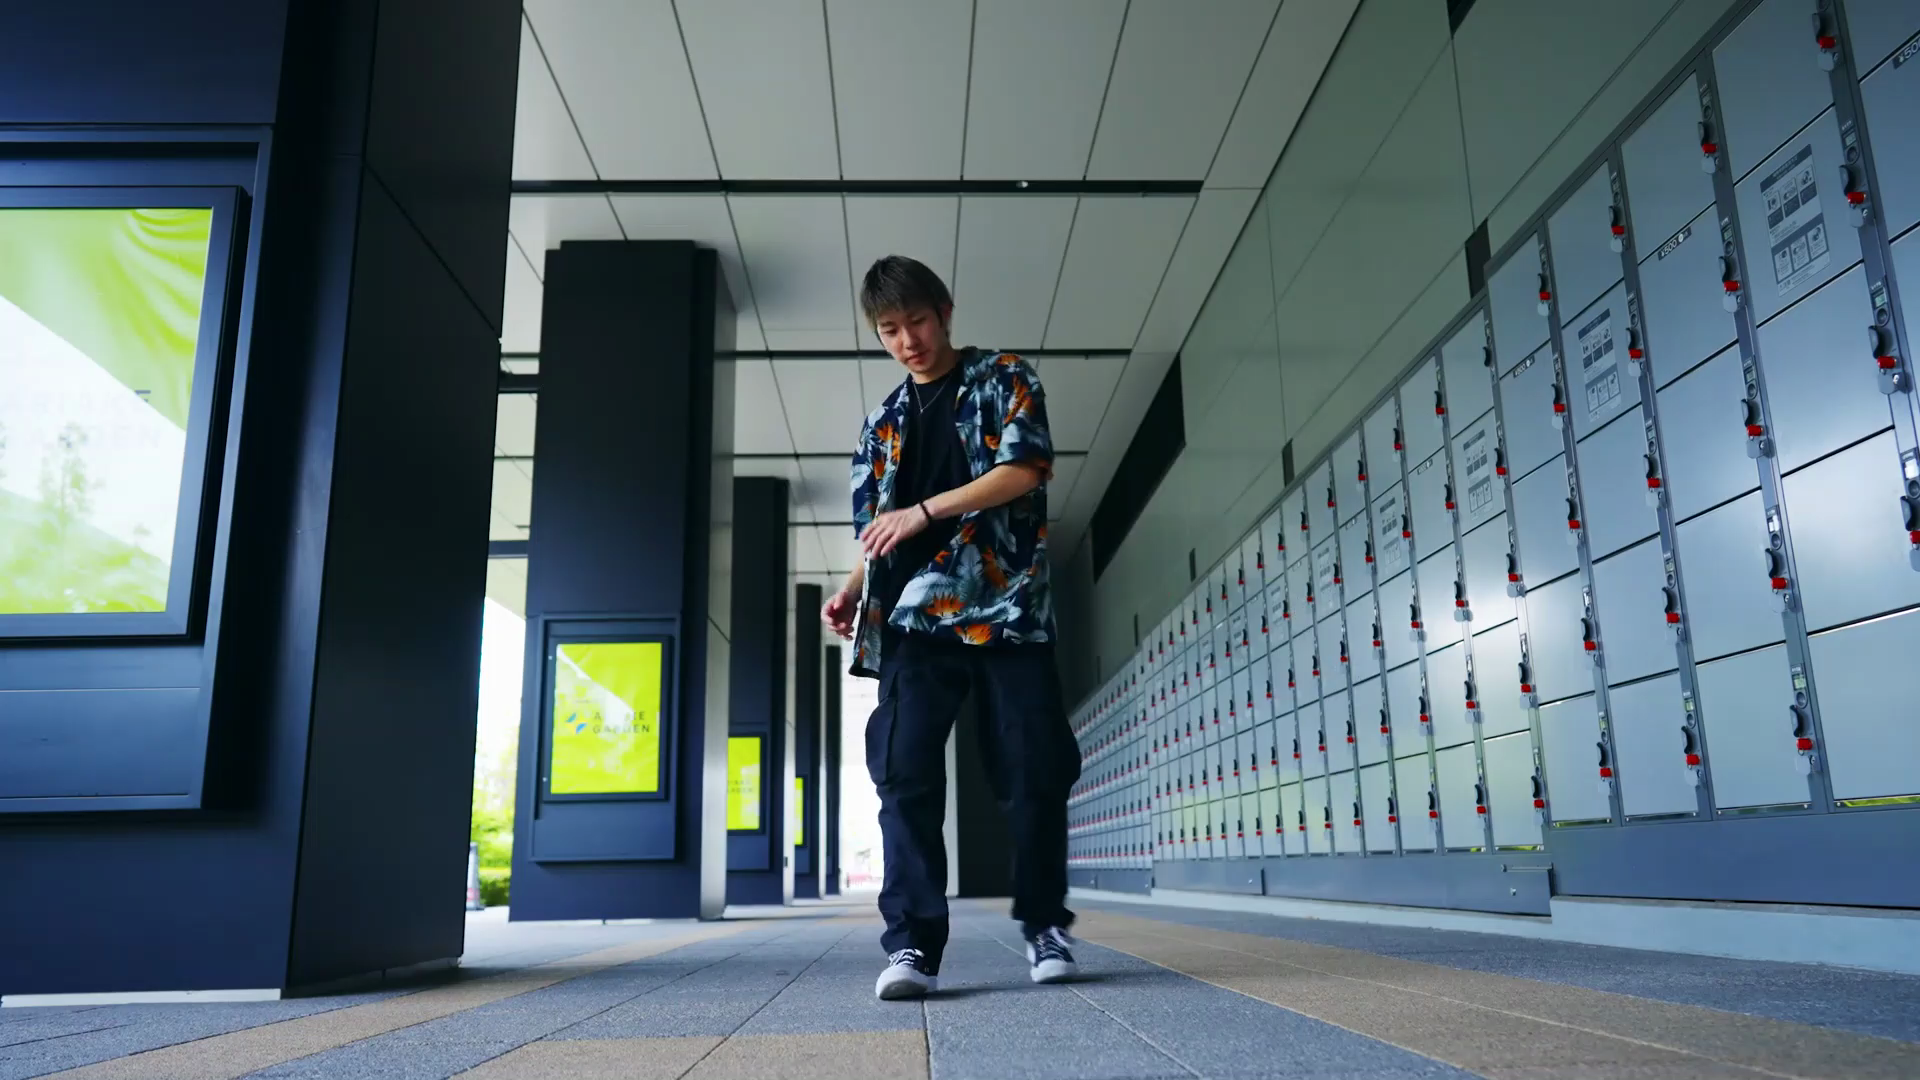
\includegraphics[width=18mm]{images/snaps/hyoga_dance.png}}
        & \multicolumn{3}{|c|}{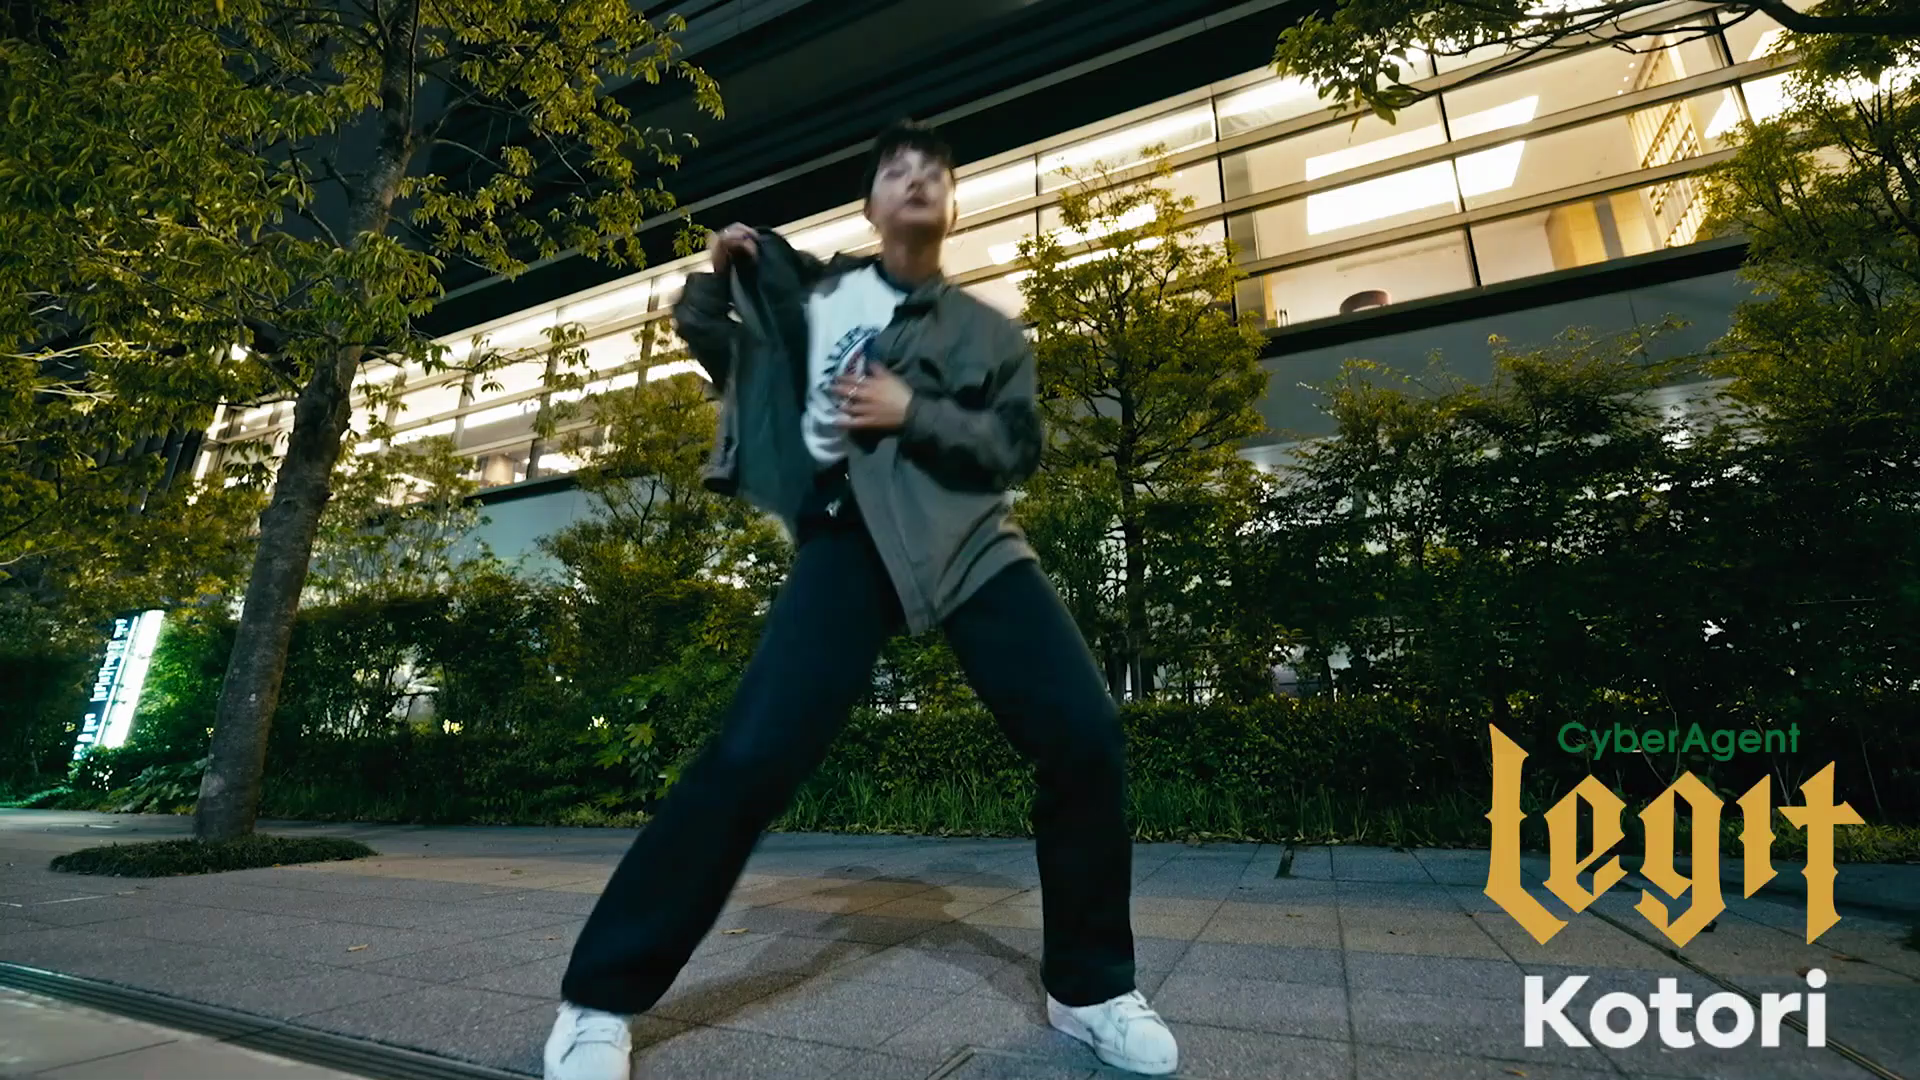
\includegraphics[width=18mm]{images/snaps/legit_dance.png}}
      \\ \cline{2-13}
        &19.6 &63.8 &54.8 & & & & & & & & & \\
        & \multicolumn{3}{|c|}{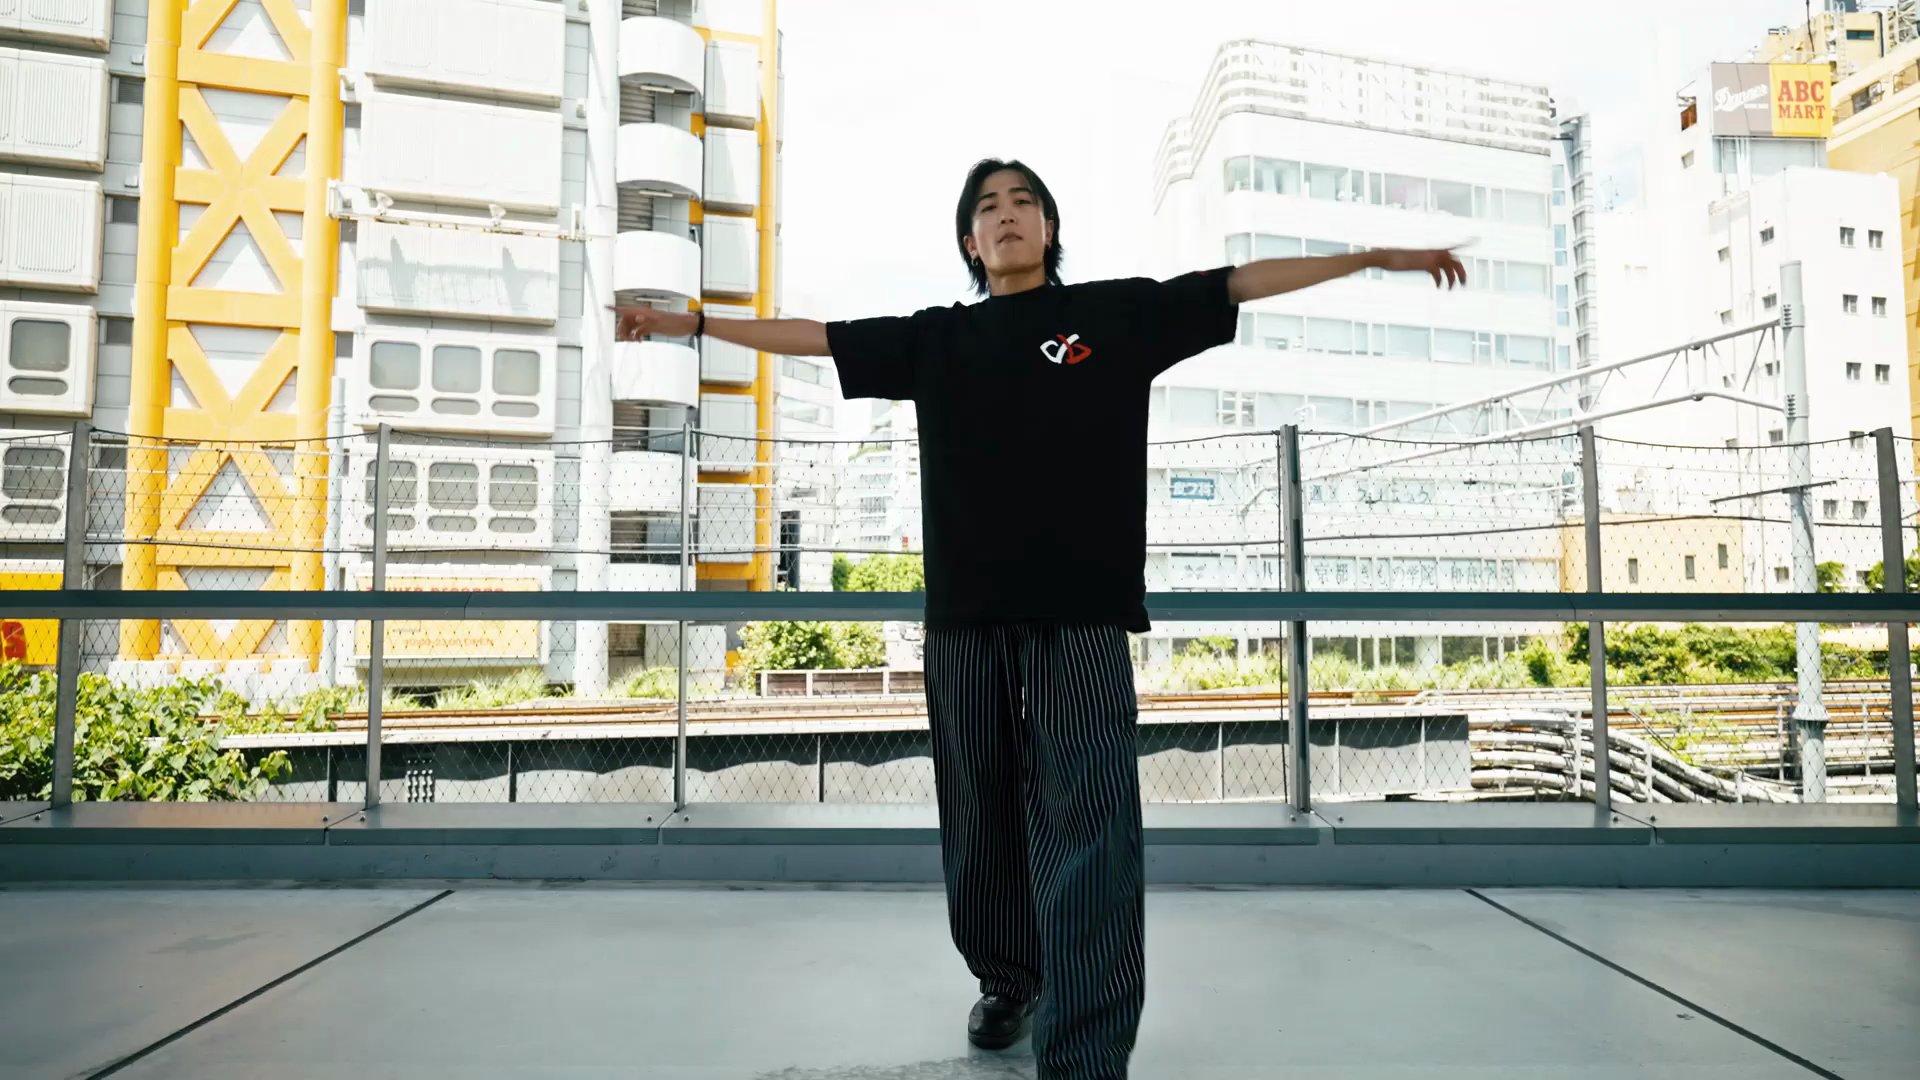
\includegraphics[width=18mm]{images/snaps/aito_dance.png}}
        & \multicolumn{3}{|c|}{}
        & \multicolumn{3}{|c|}{}
        & \multicolumn{3}{|c|}{}
      \\ \hline
        &52.6 &59.3 &21.2 &32.0 &33.3 &31.3 &41.8 &57.8 &22.3 & & & \\
        & \multicolumn{3}{|c|}{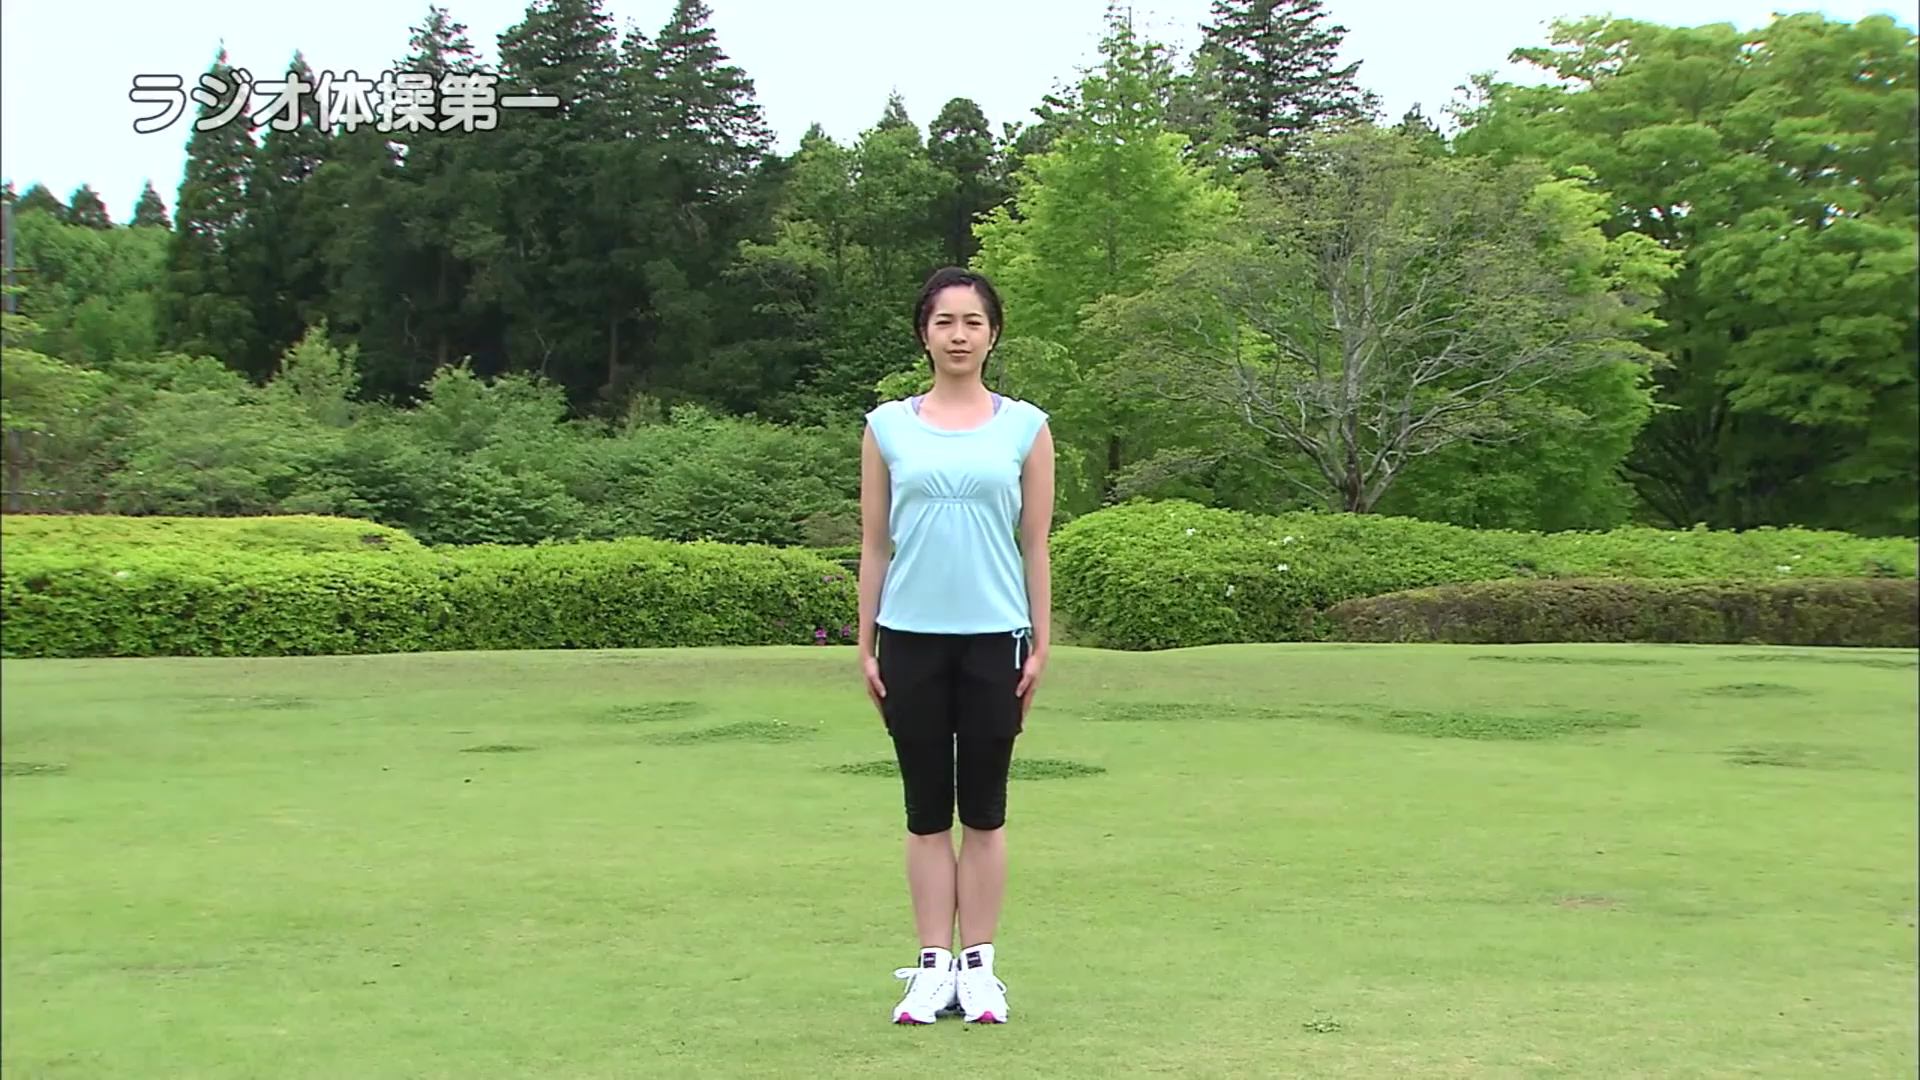
\includegraphics[width=18mm]{images/snaps/radio_exer.png}}
        & \multicolumn{3}{|c|}{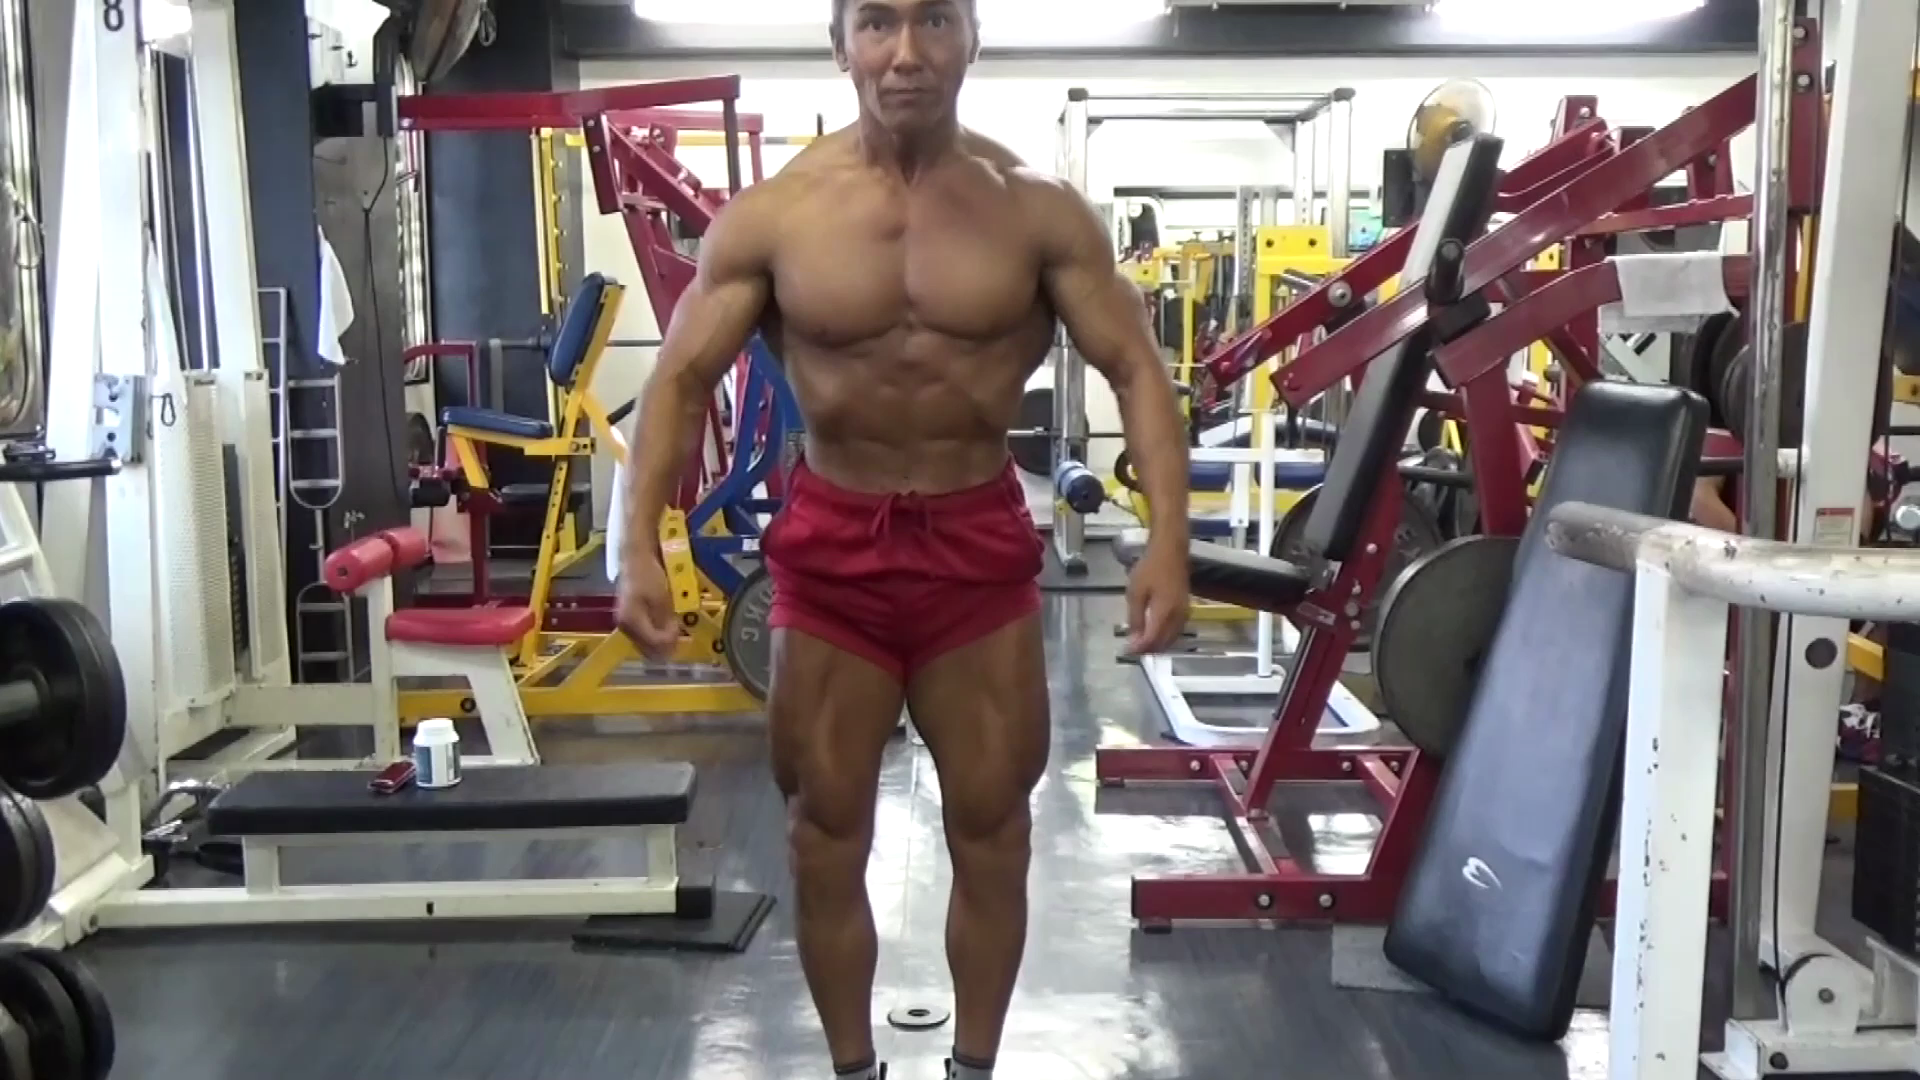
\includegraphics[width=18mm]{images/snaps/posing.png}}
        & \multicolumn{3}{|c|}{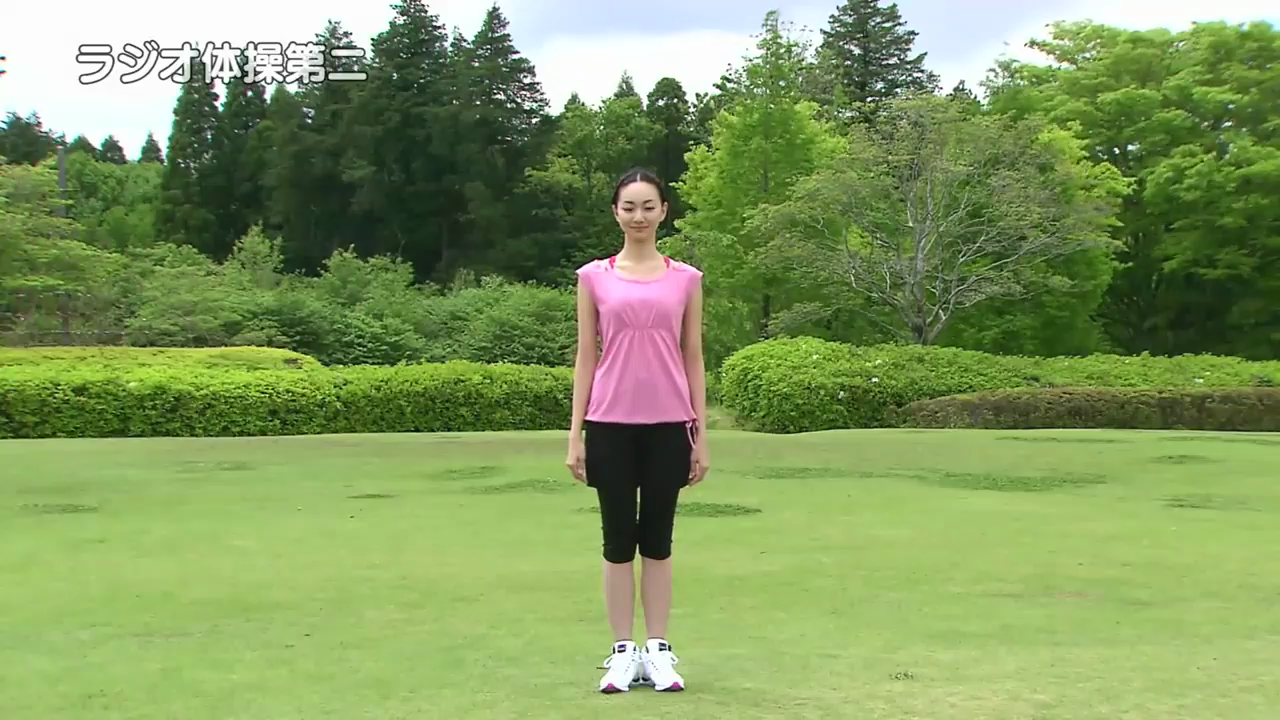
\includegraphics[width=18mm]{images/snaps/radio_exer_2.png}}
        & \multicolumn{3}{|c|}{}
      \\ \cline{2-13}
      他
        &35.4 &68.7 &78.3 &15.5 &62.3 &75.9 & & & & & & \\
        & \multicolumn{3}{|c|}{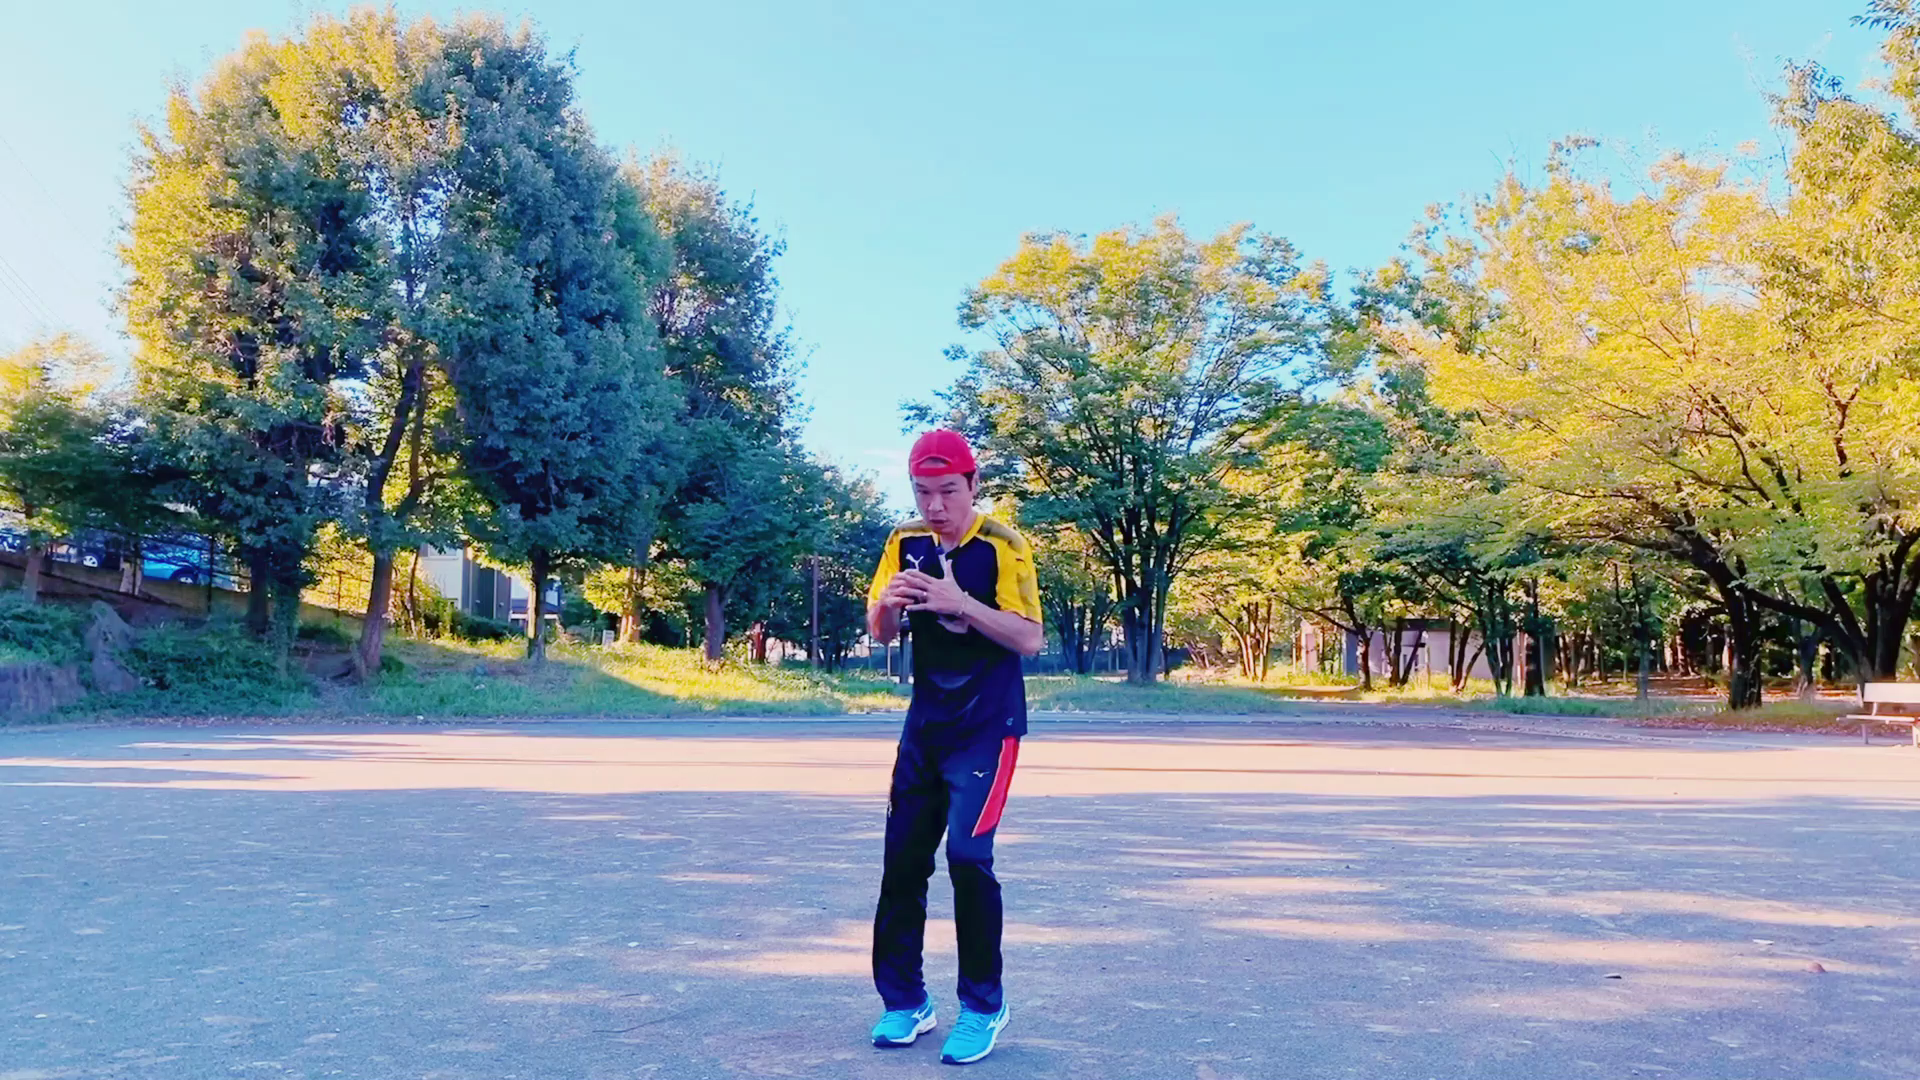
\includegraphics[width=18mm]{images/snaps/shadowboxing.png}}
        & \multicolumn{3}{|c|}{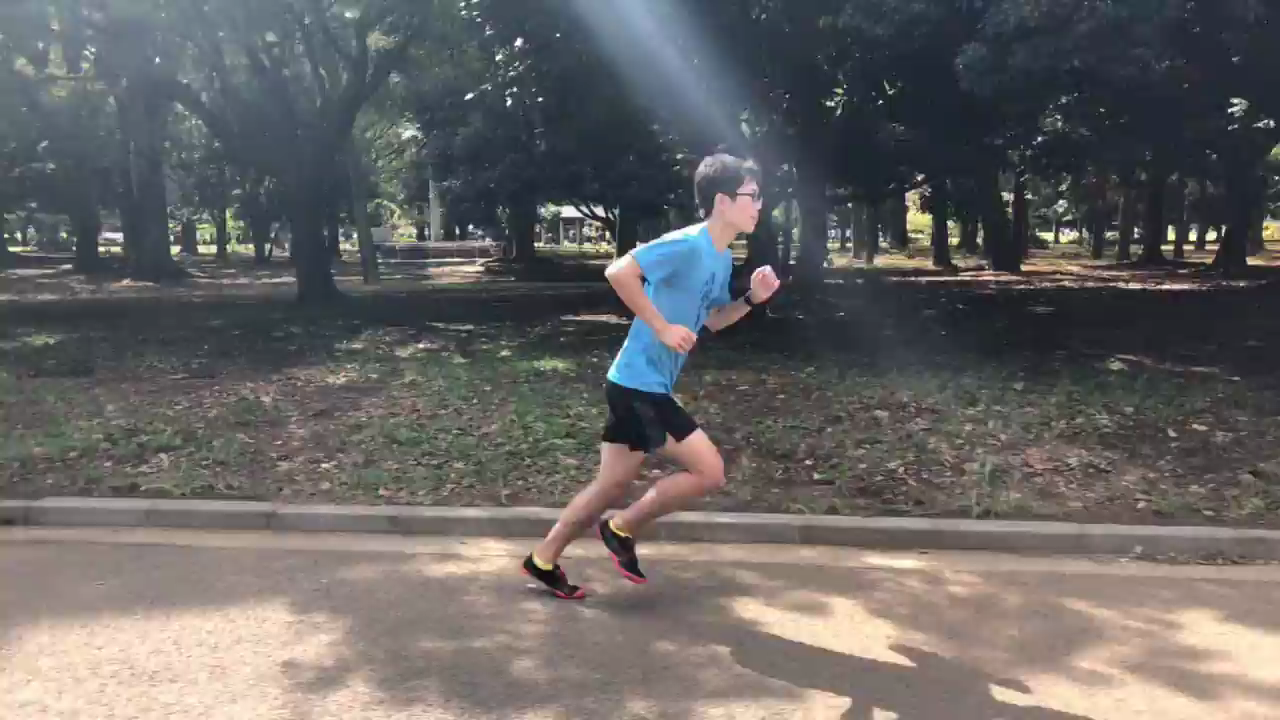
\includegraphics[width=18mm]{images/snaps/running.png}}
        & \multicolumn{3}{|c|}{}
        & \multicolumn{3}{|c|}{}
      \\ \cline{2-13}
        &81.5 &49.5 &45.2 &40.0 &52.5 &47.2 & & & & & & \\
        & \multicolumn{3}{|c|}{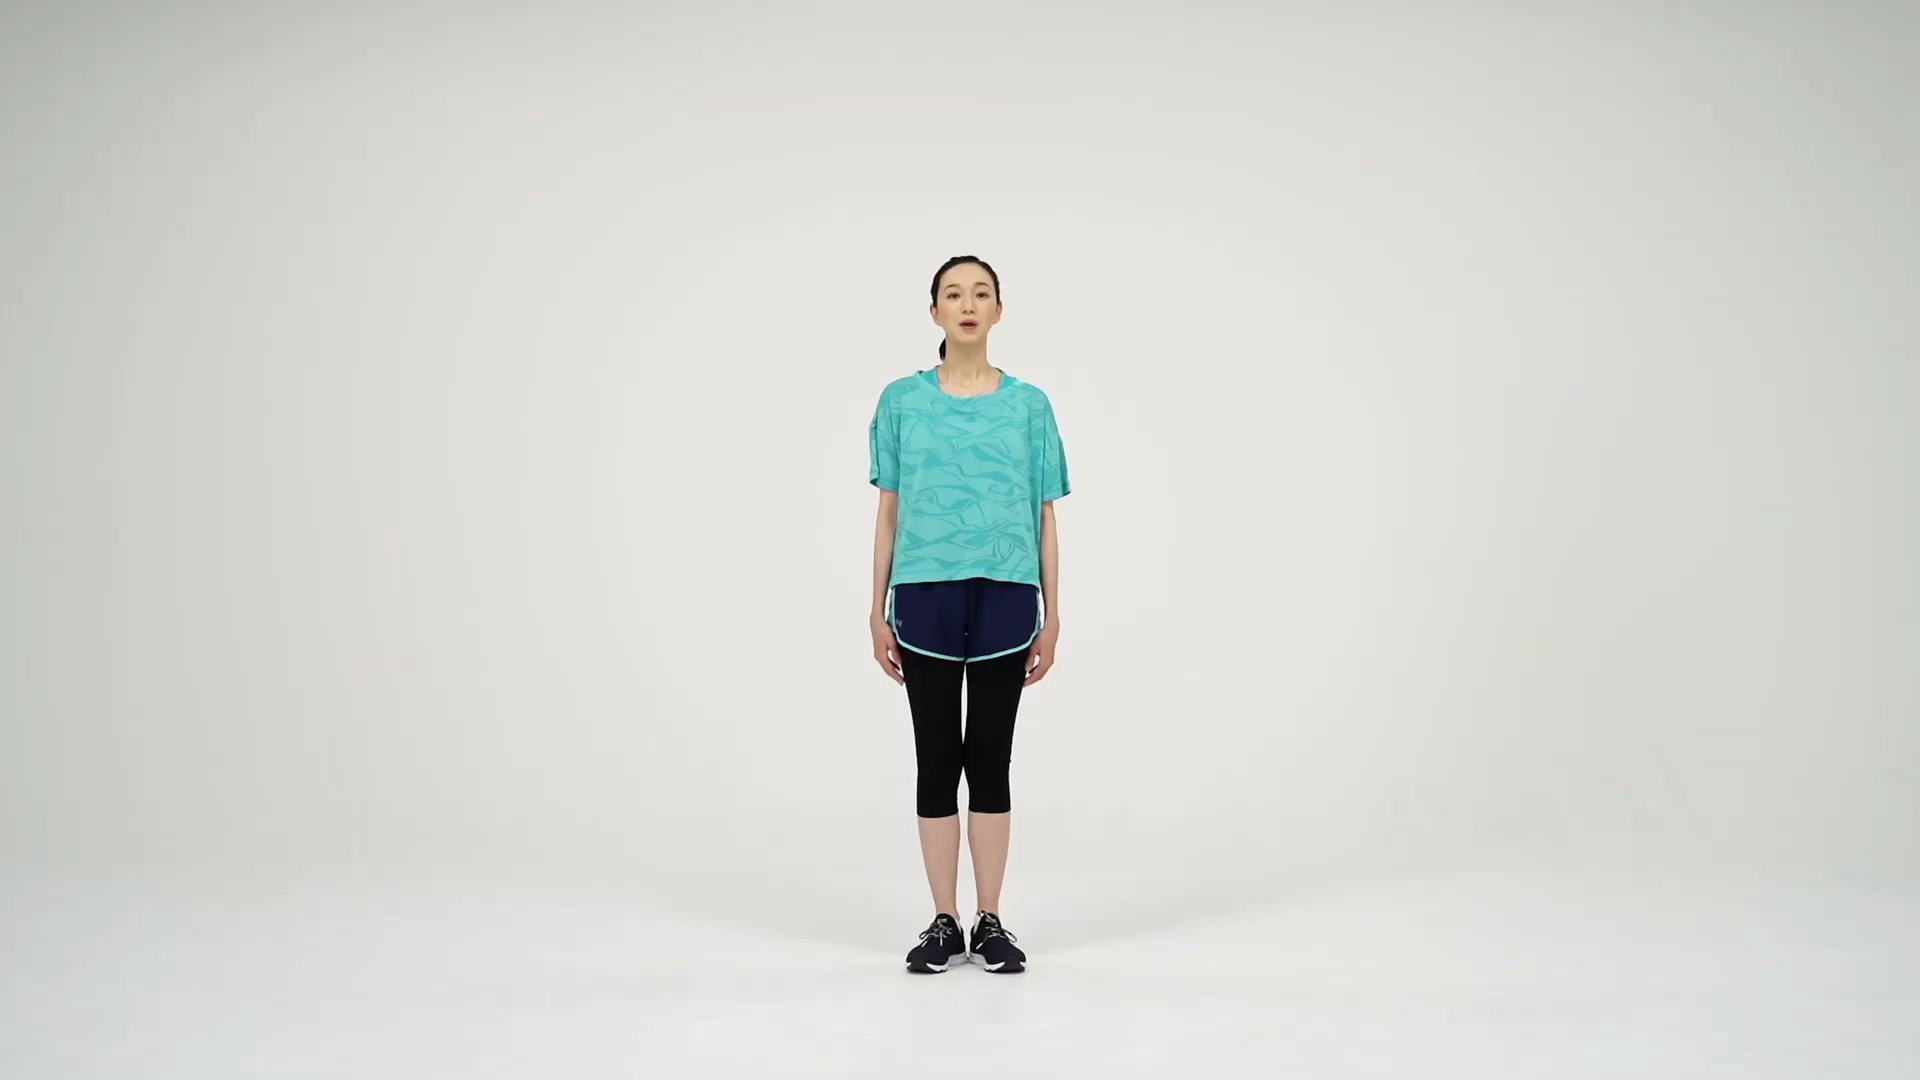
\includegraphics[width=18mm]{images/snaps/shinkokyu.png}}
        & \multicolumn{3}{|c|}{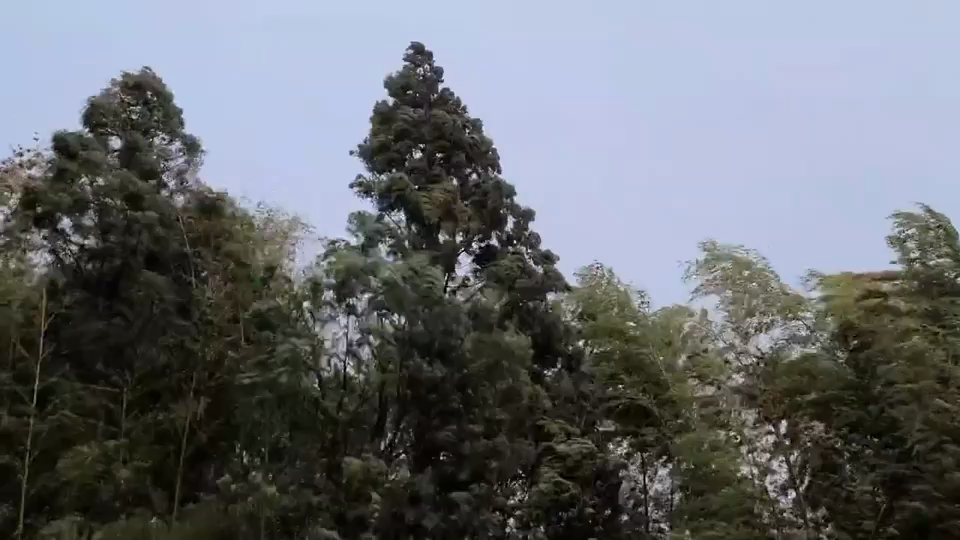
\includegraphics[width=18mm]{images/snaps/leaves.png}}
        & \multicolumn{3}{|c|}{}
        & \multicolumn{3}{|c|}{}
      \\ \hline
    \end{tabular}
  \end{center}
  \caption{算出された判断根拠分布率[%]}
  \label{devide_summary}
\end{table}
\clearpage

\subsection{確率分布を用いた評価}
別のアプローチから判断根拠を知るために,動画の確率分布を検証した.
これは動画が時間に依存したデータであることから着想を得た.
Grad Camの動画生成と同様の手法で,
図\ref{distchart}のように動画を1フレームずつ処理する.
確率分布の増減から,Grad Camより細かな判断根拠の特定と,
どのように動作するかを特定することを目指した.

ほとんどが表\ref{net_dist}のようにほとんど変化のないグラフとなったが,
精度の低いタイ舞踊では,動画の700〜800フレームに盛り上がりが見られた.
このフレームを確認すると動画のように手を大きく広げて舞踊しており,全体を通しても
優美だと感じた.クラス分類のネットワークでは出力が確率であるため
特徴を捉えることは難しかった.これは三値分類の確率であるため,
確率がほとんど1から変化しないためである.

\begin{figure}[b]
  \begin{center}
    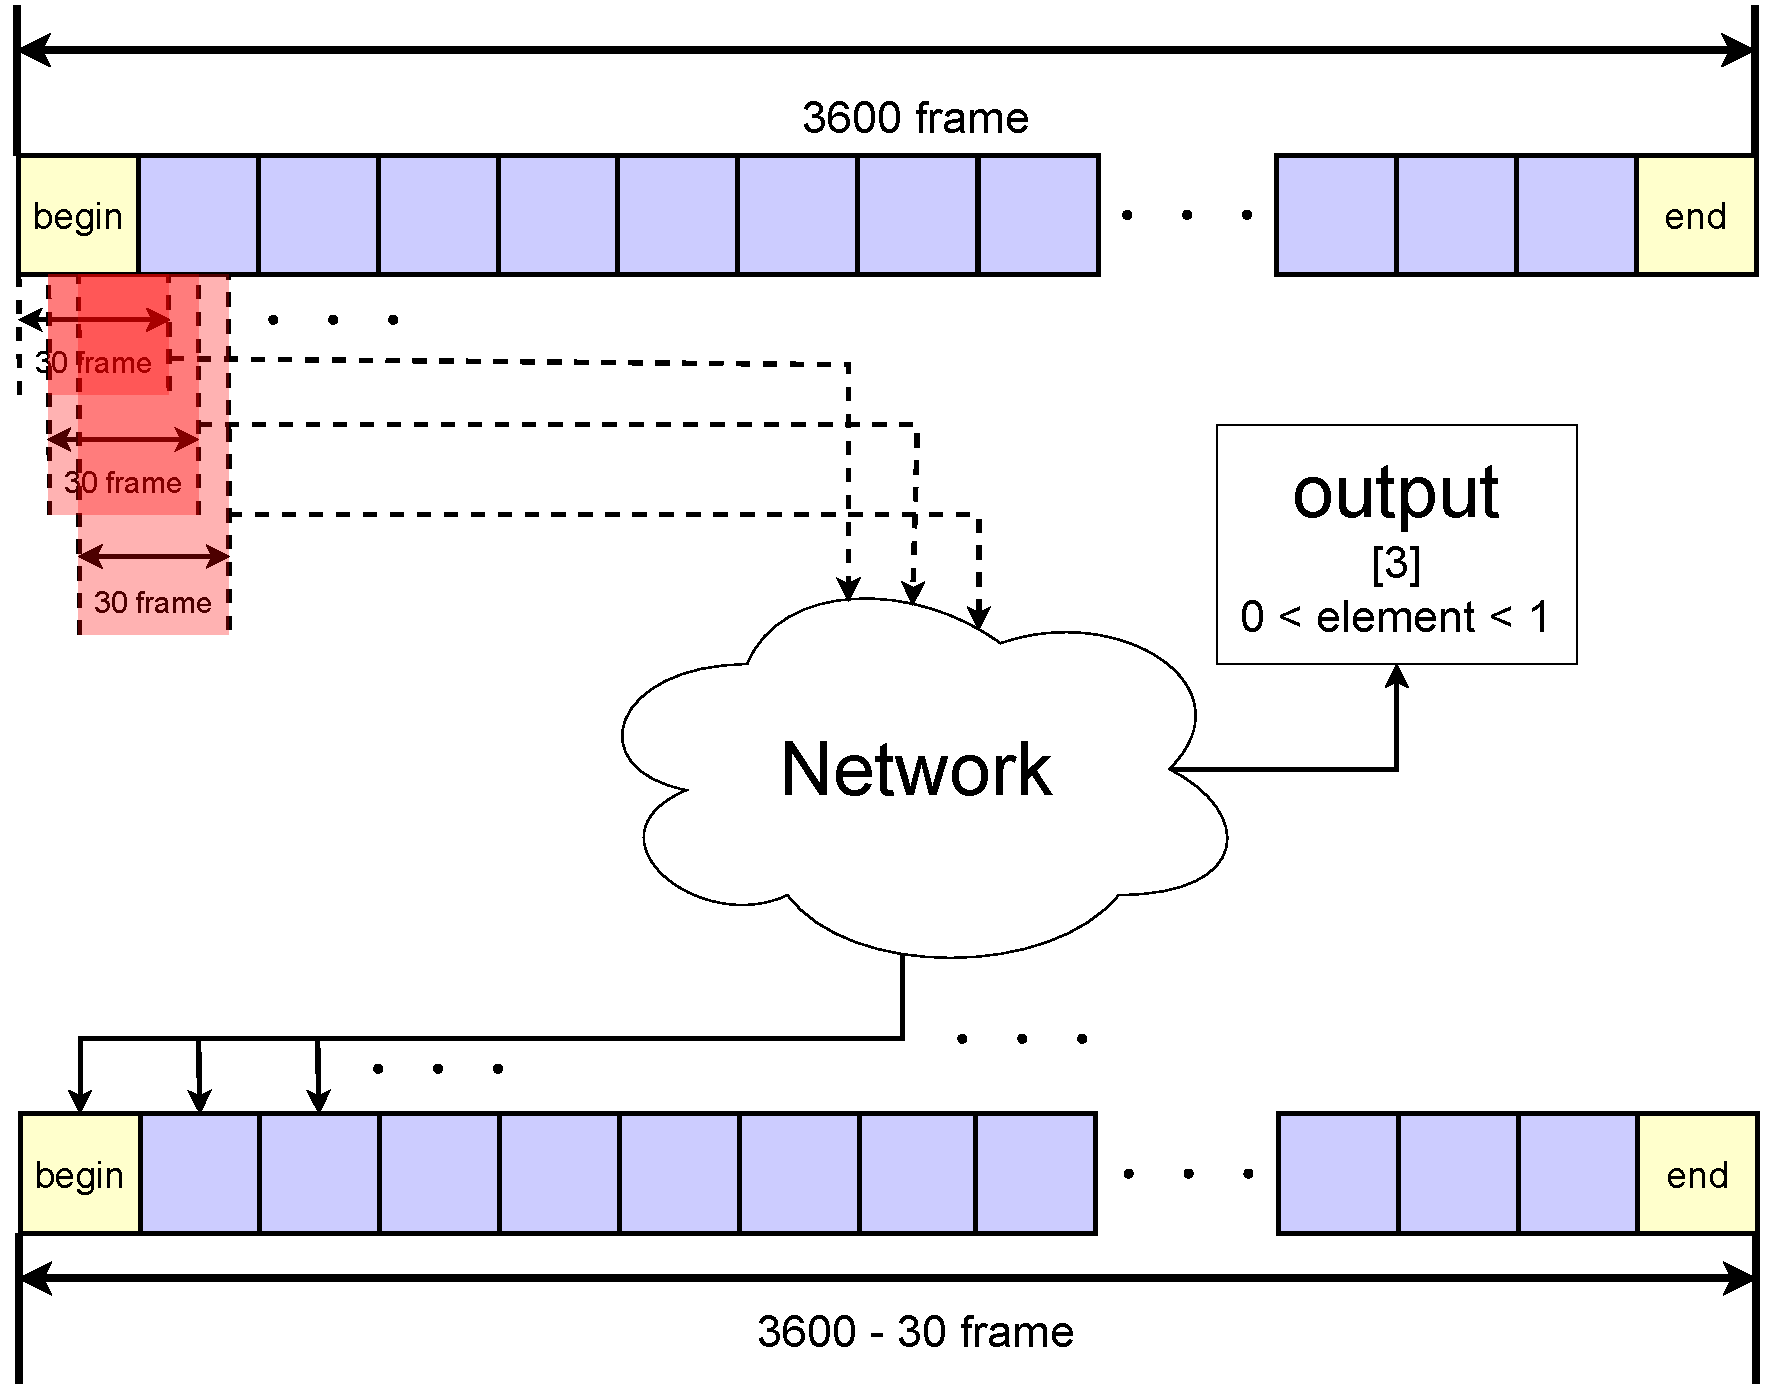
\includegraphics[width=120mm]{images/chart/net_dist.pdf}
  \end{center}
  \caption{動画長確率分布の計算方法}
  \label{distchart}
\end{figure}

\begin{table}[b]
  \begin{center}
    \begin{tabular}{c}
      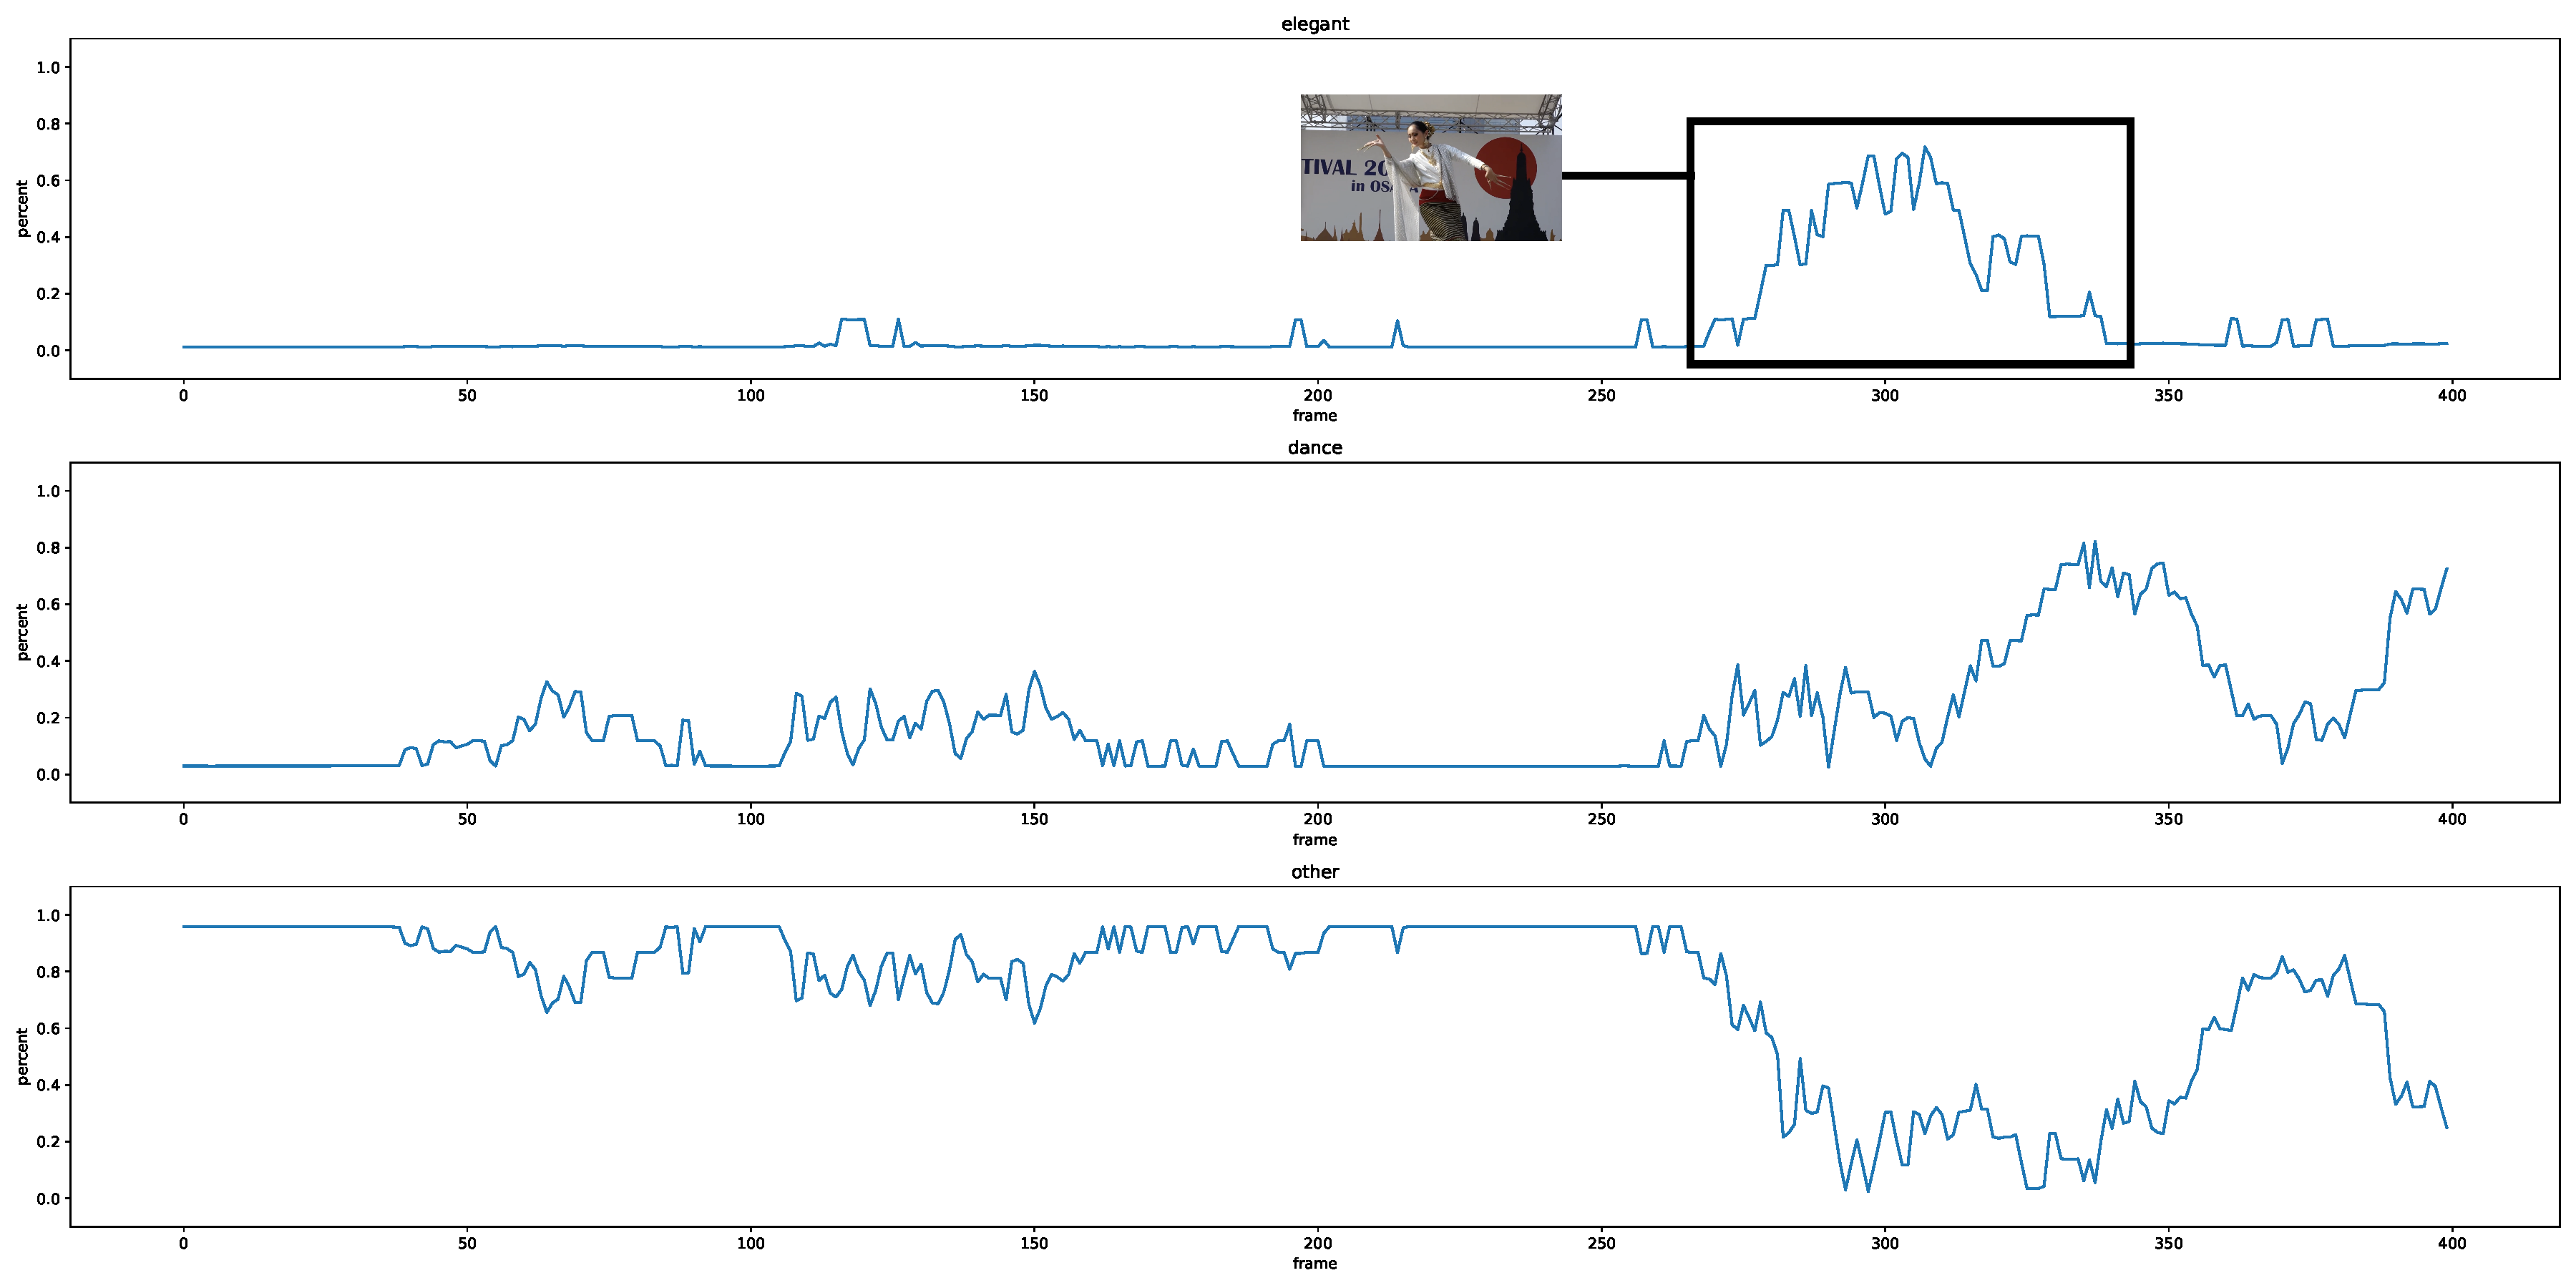
\includegraphics[width=100mm]{images/dist/thai_elegant_900.pdf} \\ タイ:500〜900 \\
      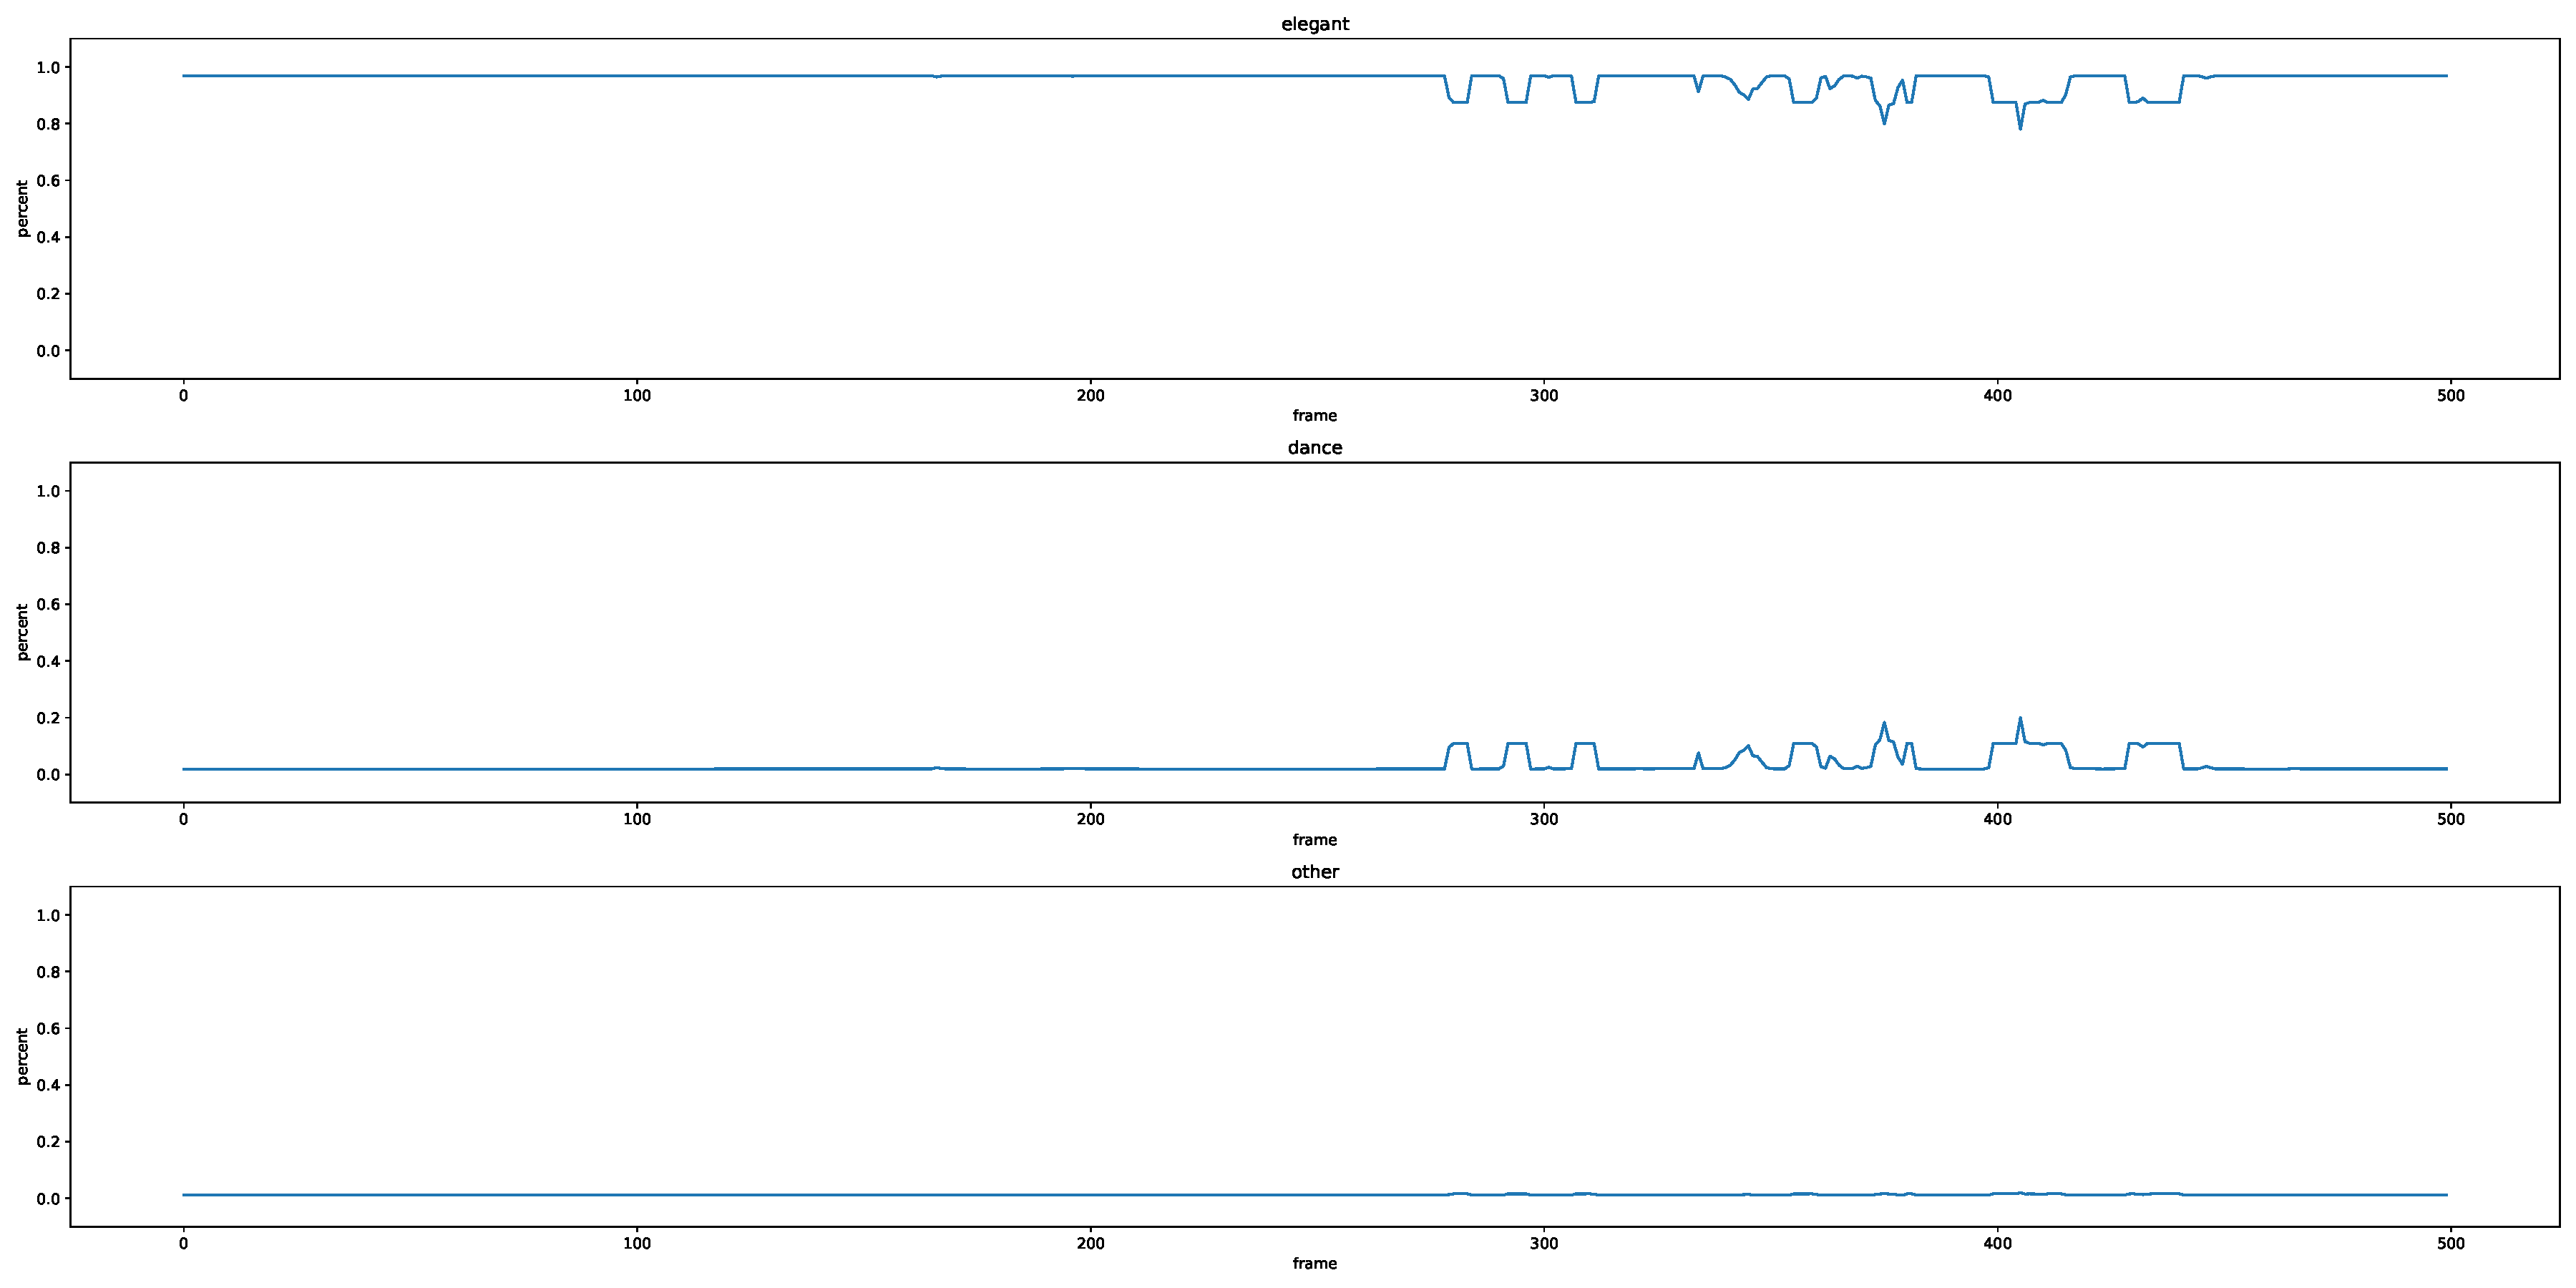
\includegraphics[width=100mm]{images/dist/japanese_elegant_2000.pdf} \\ 日本:1500〜2000 \\
      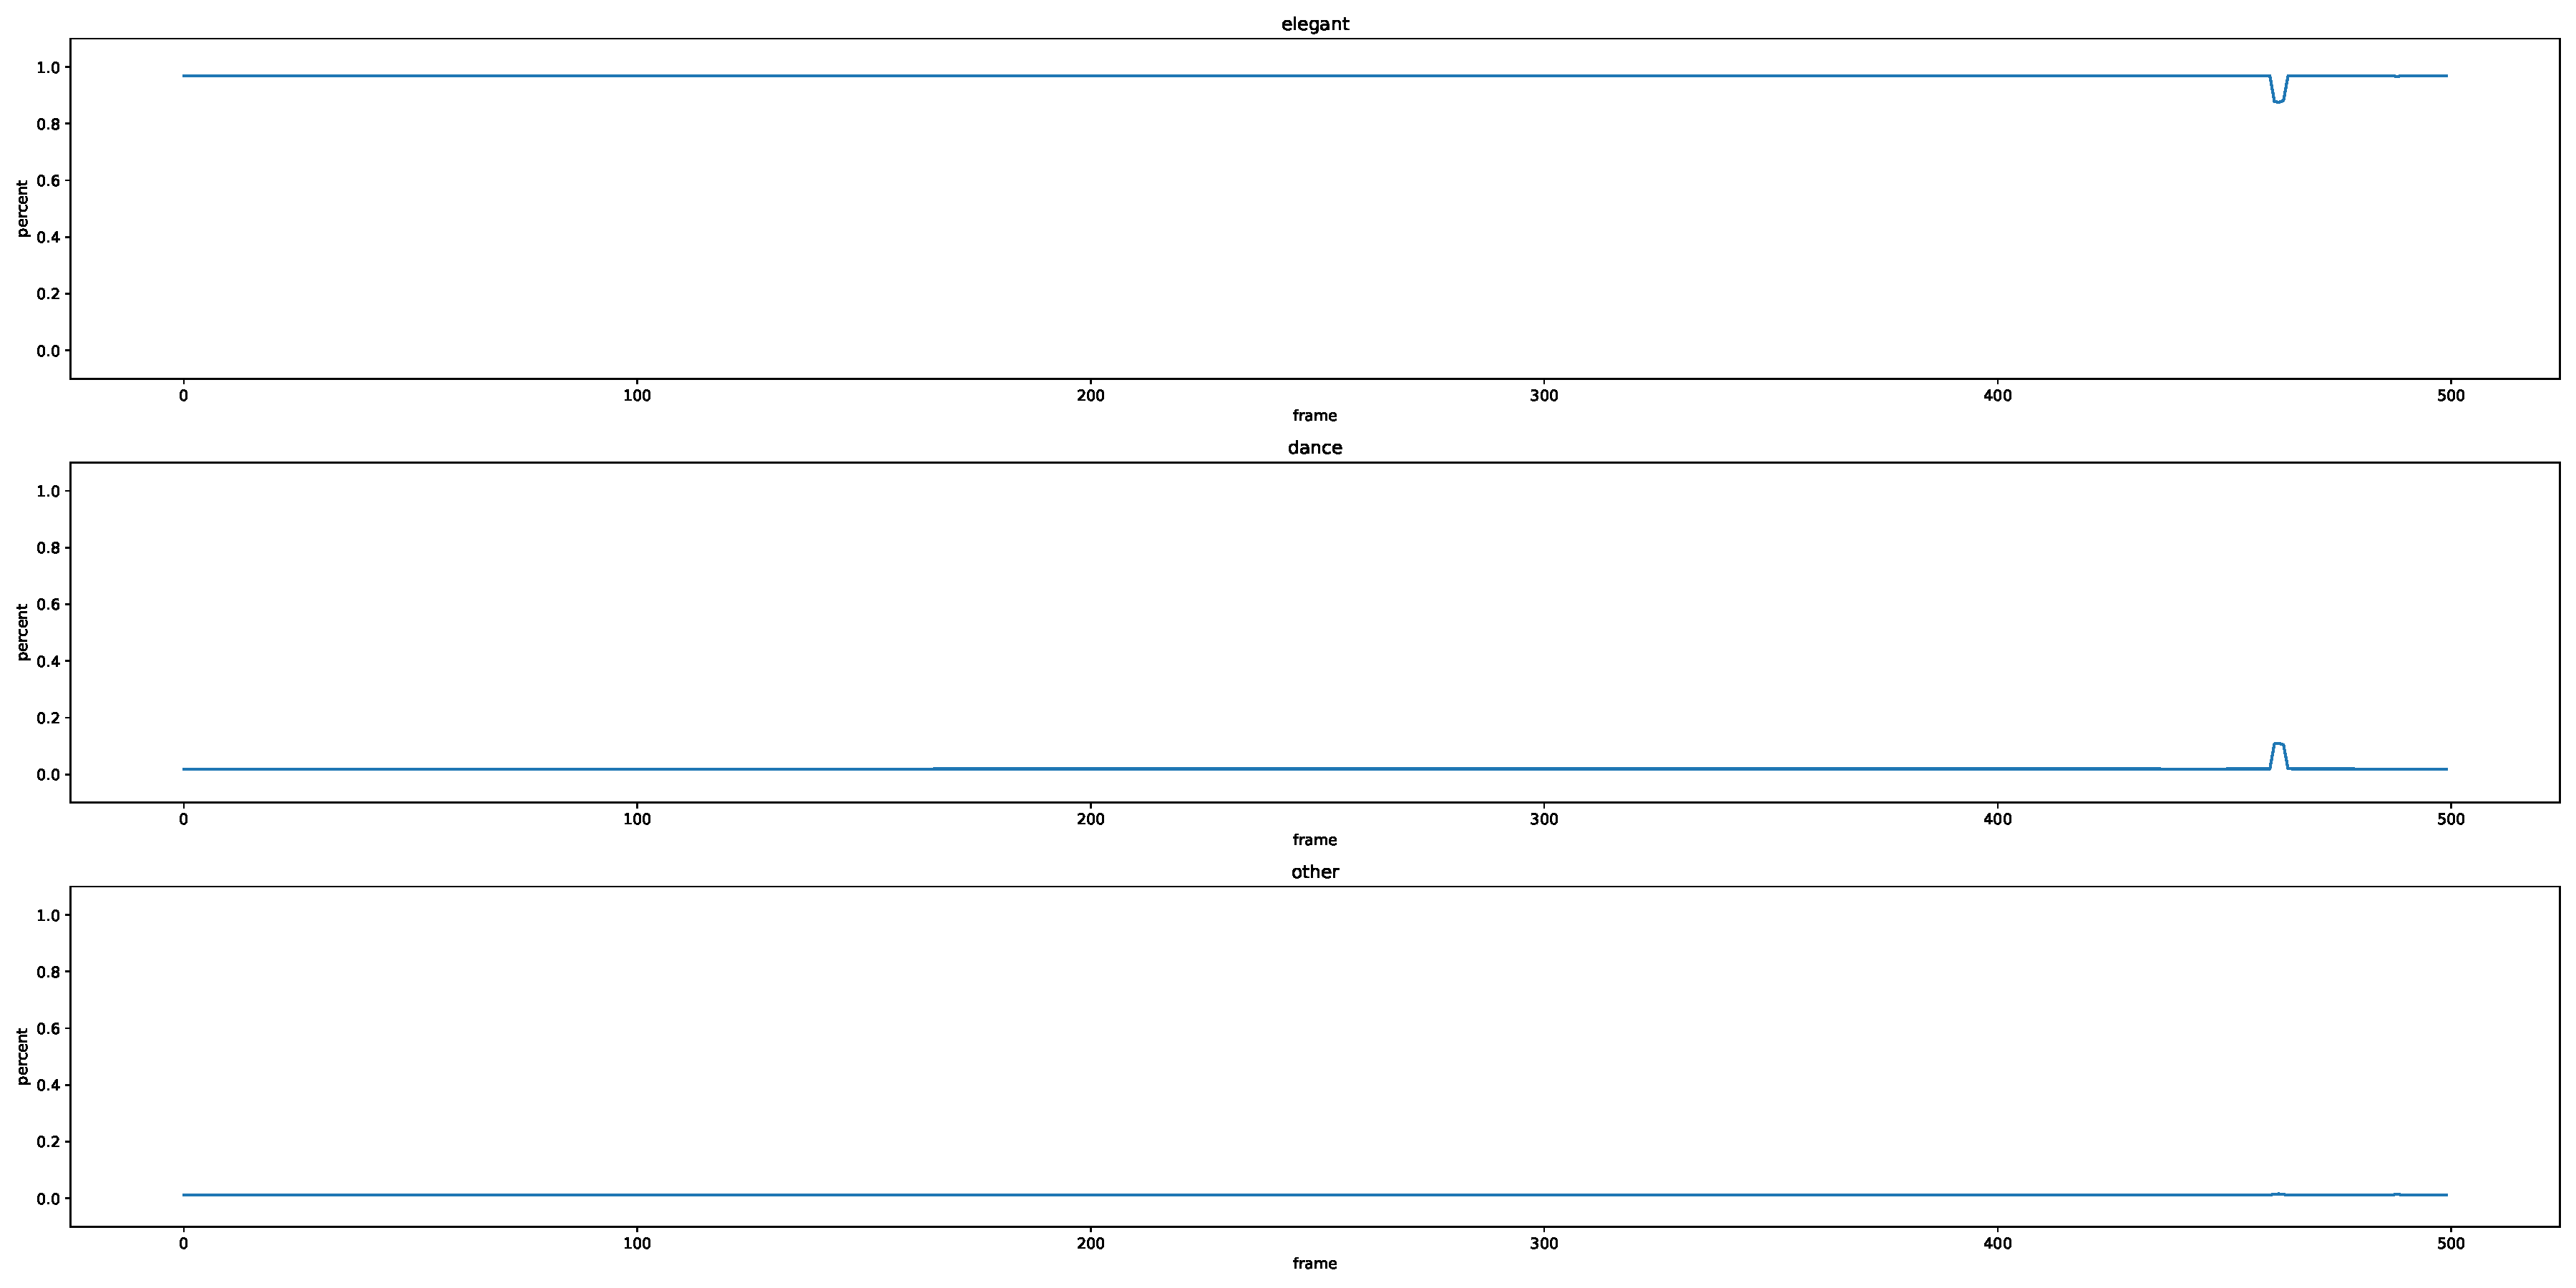
\includegraphics[width=100mm]{images/dist/chinese_elegant_1500.pdf} \\ 中国:1000〜1500 \\
    \end{tabular}
  \end{center}
  \caption{確率分布出力結果のグラフと対象舞踊フレーム数}
  \label{net_dist}
\end{table}
\clearpage

\subsection{従来手法との比較}
今回の評価では大きな成果は得られなかったが,AIを用いることで
モデルベースでは時間的,フォーマット的に扱えなかったデータを扱うことができた.
しかし,特徴を漠然としか捉えることができず,現段階では,モデルベースと学習ベースの
二つの併用運用が望ましい.

表\ref{json}のように動画から体の部位を抽出できるAIフレームワークのOpenposeを使用して手先軌道を
取得し,特徴の意図を汲み取る試みも行ったが,外れ値がデータのほとんどを占めており,
youtubeから取得した画素数の少ない動画では,手先軌道の抽出は不可能であった.
Grad Camの結果から考察した仮説である
\begin{enumerate}
  \item 優美なダンスは手足を頻繁に使う
  \item 普通のダンスは体幹移動を頻繁に使う
  \item その他の動作は確率が分散している
\end{enumerate}
が真とすると,従来研究の手先に注目する解析は
今回のモデルとも共通項があるが,足運びに注目することを提案することも可能となる.

確率分布の可視化精度の向上として挙げられることとして,分類数を増やすことや,
同じ確率の数値であっても,特徴を取り出すような手法を
開発できればその確率の特徴を見ることが可能だと考える.

\begin{table}[b]
  \begin{center}
    \begin{tabular}{c}
      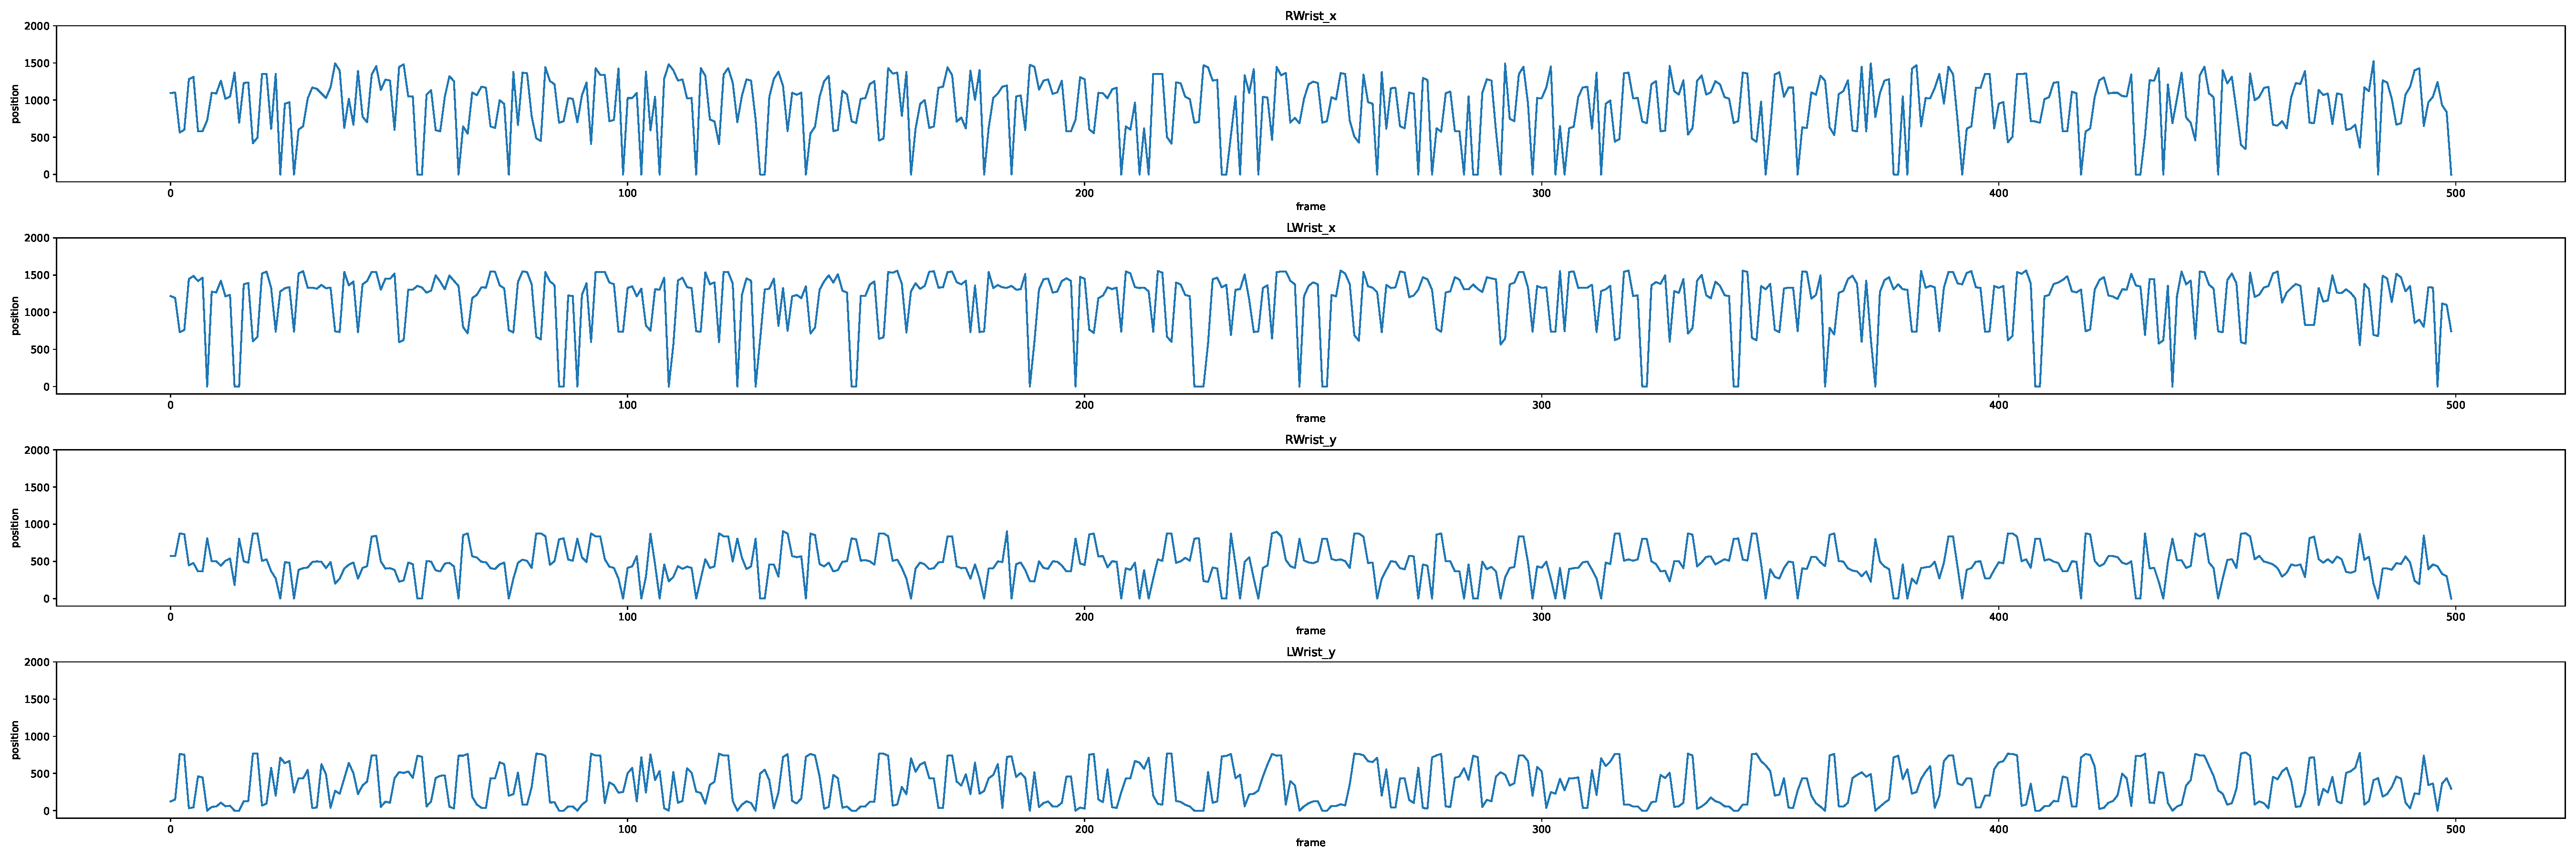
\includegraphics[width=130mm]{images/dist/thai_elegant_json.pdf} \\
    \end{tabular}
  \end{center}
  \caption{Openposeから抽出したタイ舞踊:700〜800フレームの手先起動}
  \label{json}
\end{table}
\clearpage

\section{おわりに}
\section{おわりに}

\clearpage

\bibliography{chapters/papers}
\bibliographystyle{jplain}

\end{document}
